%%%%%%%%%%%%%%%%%%%%%%%%%%%%%%%%%%%%%%%%%%%%%%%%%%%%%%%%%%%%%%%%%%%%%%%%%%%%%%%%%%%%%
\section{Introduction} \label{sec:gd_intro}
%%%%%%%%%%%%%%%%%%%%%%%%%%%%%%%%%%%%%%%%%%%%%%%%%%%%%%%%%%%%%%%%%%%%%%%%%%%%%%%%%%%%%

The field of astrophysics now has several instruments and observatories sensitive to high energy gamma-rays.
The energy sensitivity for the modern gamma-ray program spans many orders of magnitude.
\Cref{fig:gd_motivation} demonstrates these comparable sensitivities across energies for the five experiments: Fermi-LAT, HAWC, HESS, MAGIC, and VERITAS.

\begin{figure}[t]
    \centering{
        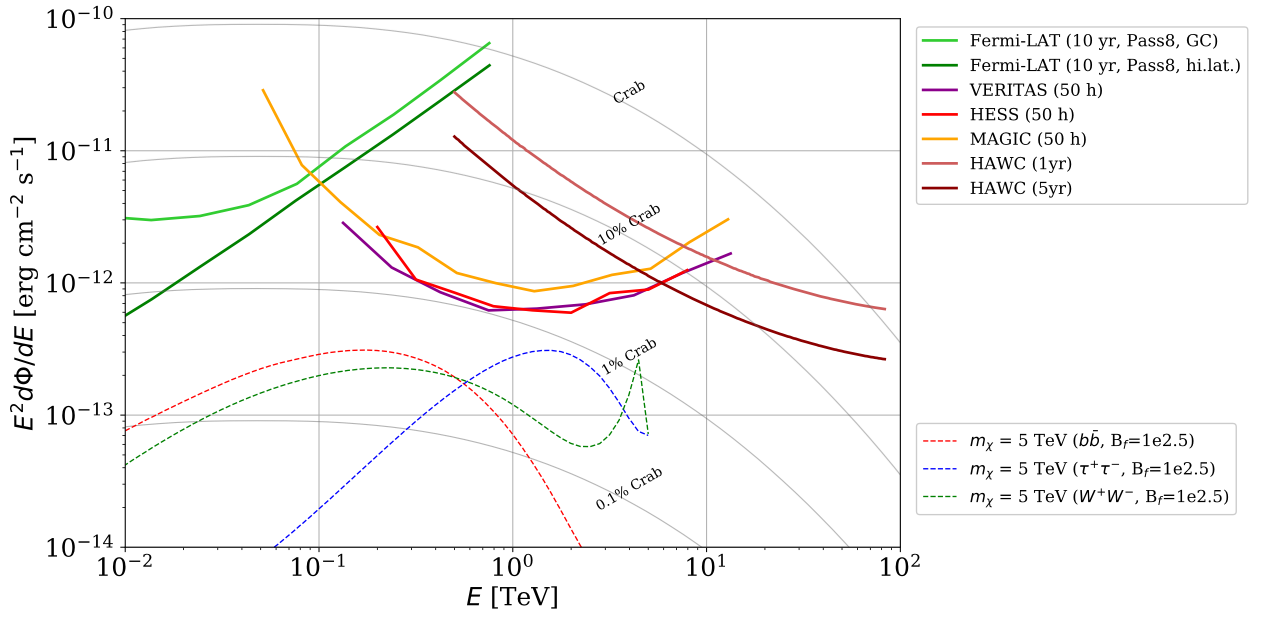
\includegraphics[scale=0.35]{figures/glory_duck/gd_motivation.png}
    }
    \caption{Sensitivities of five gamma-ray experiments compared to percentages of the Crab nebula's emission and dark matter annihilation. Solid lines present estimated sensitivities to power law spectra \fu for each experiment. Green lines are Fermi-LAT sensitivities where lighter green is the sensitivity to the galactic center and dark green is its sensitivity to higher declinations. Orange, red, and purple solid lines represent the MAGIC, HESS, and VERITAS 50 hour sensitivities respectively. The maroon and brown lines are the HAWC 1 year and 5 year sensitivities. Across four decades of gamma-ray energy, these experiments have similar sensitivities on the order $10^{-12}$ erg cm$^{-2}$s$^{-1}$. The dotted lines are estimated dark matter fluxes assuming $m_{\chi} = 5$~TeV DM annihilating to bottom quarks (red), tau leptons (blue), and W bosons (green). Faded gray lines outline percentage flux of the Crab nebula. Figure is an augmented version of \cite{2020Galax...8...25R}}
    \label{fig:gd_motivation}
\end{figure}

Each of the five experiments featured in \Cref{fig:gd_motivation} have independently searched for DM annihilation from dwarf spheroidal galaxies (dSph) and set limits on annihilation cross-section of WIMPs.
Intriguingly, there are regions of substantial overlap in their energy sensitivities.
This clearly motivates an analysis that combines data from these five.
Each experiment has unique gamma-ray detection methods and their weaknesses and strengths can be leveraged with each other.
The HAWC gamma-ray observatory is extensively introduced in \Cref{sec:hawc}, so it is not introduced here.
A brief description of the remaining experiments are in the following paragraphs.

The Large Area Telescope (LAT) is a pair conversion telescope mounted on the NASA Fermi satellite in orbit $\sim$550 km above the Earth \cite{FermiLAT}.
LAT's field of view covers about 20\% of the whole sky, and it sweeps the whole sky approximately every 3 hours.
LAT's gamma-ray energy sensitivity ranges from 20 MeV up to 1 TeV.
Previous DM searches towards dSphs using Fermi-LAT are published in \cite{FermiLAT:dm1} and \cite{FermiLAT:dm2}.

\sloppy The High Energy Spectroscopic System (HESS), Major Atmospheric Gamma Imaging
Cherenkov (MAGIC), and Very Energetic Radiation Imaging Telescope Array System (VERITAS) are arrays of Imaging Atmospheric Cherenkov Telescopes (IACT).
These telescopes observe the Cherenkov light emitted from gamma-ray showers in the Earth's atmosphere.
The field of view for these telescopes is no larger than $5\degree$ with energy sensitivities ranging from ~ 30 GeV up to 100 TeV \cite{HESS,MAGIC,VERITAS}.
IACTs are able to make precise observations in selected regions of the sky, however can only be operated in ideal dark conditions.
HESS's  observations of the dwarves Sculptor and Carina were between January 2008 and December 2009.
HESS's observations of Coma Berenices were taken from 2010 to 2013, and Fornax was observed in 2010 \cite{HESS:dm_sculptor_carina,HESS:dm_dwarves,HESS:dm_gamma_lines}.
MAGIC provided deep observations of Segue1 between 2011 and 2013 \cite{MAGIC:dm_segue1}.
MAGIC also provides data for three additional dwarves: Coma Berenices, Draco, and Ursa Major II where observations were made in: January - June 2019 \cite{MAGIC:dm_comab_draco}, March - September 2018 \cite{MAGIC:dm_comab_draco}, and 2014 - 2016 \cite{MAGIC:dm_uma2} respectively.
VERITAS provided data for Boötes I, Draco, Segue 1, and Ursa Minor from 2009 to 2016 \cite{VERITAS:dm_dwarves}.

This chapter presents the Glory Duck analysis, the name given for the search for dark matter annihilation from dSph by combining data from the five gamma-ray observatories: Fermi-LAT, HAWC, HESS, MAGIC, and VERITAS.
Specifically, the methods in analysis and modeling are presented for the HAWC gamma-ray observatory.
This work will be published in the Journal of Cosmology and Astroparticle Physics and presented at the International Cosmic Ray Conference in 2019, 2021, and 2023 \cite{glory_duck:ICRC2019,glory_duck:ICRC2021,glory_duck:ICRC2023} and others.

%%%%%%%%%%%%%%%%%%%%%%%%%%%%%%%%%%%%%%%%%%%%%%%%%%%%%%%%%%%%%%%%%%%%%%%%%%%%%%%%%%%%%
\section{Dataset and Background}\label{sec:gd_databgd}
%%%%%%%%%%%%%%%%%%%%%%%%%%%%%%%%%%%%%%%%%%%%%%%%%%%%%%%%%%%%%%%%%%%%%%%%%%%%%%%%%%%%%

This section enumerates the data analysis and background estimation methods used for HAWC's study of dSphs.
\Cref{sec:gd_data} and \Cref{sec:gd_tools} are most useful for fellow HAWC collaborators looking to replicate the Glory Duck analysis.

%%%%%%%%%%%%%%%%%%%%%%%%%%%%%%%%%%%%%%%%%%%%%%%
\subsection{Itemized HAWC files}\label{sec:gd_data}
%%%%%%%%%%%%%%%%%%%%%%%%%%%%%%%%%%%%%%%%%%%%%%%
These files are only available withing HAWC's internal documentation and collaborators.
They are not meant for public access, and are presented here so that HAWC collaborators can reproduce results accurately.

\begin{itemize}
    \item Detector Response: \url{response\_aerie\_svn\_27754\_systematics\_best\_mc\_test\_nobroadpulse\\
    \_10pctlogchargesmearing\_0.63qe\_25kHzNoise\_run5481\_curvature0\_index3.root}
    \item Data Map: \texttt{maps-20180119/liff/maptree\_1024.root}
    \item Spectral Dictionary: \texttt{DM\_CirrelliSpectrum\_dict\_gammas.npy}
    \item Analysis wiki: \url{https://private.hawc-observatory.org/wiki/index.php/Glory_Duck_Multi-Experiment_Dark_Matter_Search}
\end{itemize}

% %%%%%%%%%%%%%%%%%%%%%%%%%%%%%%%%%%%%%%%%%%%%%%%
\subsection{Software Tools and Development}\label{sec:gd_tools}
%%%%%%%%%%%%%%%%%%%%%%%%%%%%%%%%%%%%%%%%%%%%%%%

This analysis was performed using HAL and 3ML \cite{Abeysekara_2017, vianello2015multimission} in Python version 2.
I built software to implement the \emph{A Poor Particle Physicist Cookbook for Dark Matter Indirect Detection} (PPPC) \cite{Cirelli_2011} DM spectral model and dSphs spatial model from \cite{Geringer_Sameth_2015} for HAWC analysis.
A NumPy version of this dictionary was made for both Py2 and Py3.
The code base for creating this dictionary is linked on my GitLab sandbox:

\begin{itemize}
    \item Py2: \href{https://gitlab.com/hawc-observatory/sandboxes/salaza82/glory-duck-hawc/-/tree/master/GD_spectrum}{Dictionary Generator (Deprecated)}
    \item Py3: \href{https://gitlab.com/hawc-observatory/sandboxes/salaza82/pppc2dict}{PPPC2Dict}
\end{itemize}

The analysis was performed using the $f_{\textrm{hit}}$ framework as used and described in the HAWC Crab paper \cite{Abeysekara_2017}.
The Python2 NumPy dictionary file for gamma-ray final states is \texttt{dmCirSpecDict.npy}.
The corresponding Python3 file is \texttt{DM\_CirrelliSpectrum\_dict\_gammas.npy}.
These files can also be used for decay channels and the PPPC describes how \cite{Cirelli_2011}.
All other software used for data analysis, DM profile generation, and job submission to SLURM are also kept in my sandbox for \href{https://gitlab.com/hawc-observatory/sandboxes/salaza82/glory-duck-hawc}{the Glory Duck} project.

%%%%%%%%%%%%%%%%%%%%%%%%%%%%%%%%%%%%%%%%%%%%%%%
\subsection{Data Set and Background Description} \label{sec:gs_data_bkgd}
%%%%%%%%%%%%%%%%%%%%%%%%%%%%%%%%%%%%%%%%%%%%%%%

The HAWC data maps used for this analysis contain 1017 days of data between runs 2104 (2014-11-26) and 7476 (2017-12-20).
They were generated from pass 4.0 reconstruction.
The analysis is performed using the $f_{hit}$ energy binning scheme with bins (1-9) similar to what was done for the Crab and previous HAWC dSph analysis \cite{Abeysekara_2017,Albert_2018}.
Bin 0 was excluded as it has substantial hadronic contamination and poor angular resolution.

This analysis was done on dSphs because of their large DM mass content relative to baryonic mass.
We consider the following to estimate the background to this study.

\begin{itemize}
    \item The dSphs' angular extent are small relative to HAWC's spatial resolution, so the analysis is not sensitive to large or small scale anisotropies.
    \item The dSphs used in this analysis are off the galactic plane and therefore not contaminated by diffuse emission from the galaxy.
    \item The dSphs are baryonically faint relative to their expected dark matter content and are not expected to contain high energy gamma-ray sources.
\end{itemize}

Therefor we make no additional assumptions on the background from our sources and use HAWC's standard direct integration method for background estimation \cite{Abeysekara_2017}.
The largest background under this consideration is from an isotropic flux of cosmic rays.
The contamination of this hadronic flux is worse at lower energies where HAWC's gamma/hadron discrimination worse.
It is possible for gamma rays from DM annihilation to scatter in transit to HAWC via Inverse Compton Scattering (ICS).
This was investigated and its impact on the flux is negligible.
Supporting information on this is in \Cref{sec:gd_ics}

%%%%%%%%%%%%%%%%%%%%%%%%%%%%%%%%%%%%%%%%%%%%%%%%%%%%%%%%%%%%%%%%%%%%%%%%%%%%%%%%%%%%%
\section{Analysis}\label{sec:gd_analysis}
%%%%%%%%%%%%%%%%%%%%%%%%%%%%%%%%%%%%%%%%%%%%%%%%%%%%%%%%%%%%%%%%%%%%%%%%%%%%%%%%%%%%%

The expected differential photon flux from DM-DM annihilation to standard model
particles, $d\Phi_{\gamma}/dE_{\gamma}$, over solid angle, $\Omega$, is described by the familiar equation.
\iddmannilation[\gamma]

Where \sv~is the velocity weighted annihilation cross-section.
$\frac{dN}{dE}$ is the expected differential number of photons produced at each energy per annihilation.
$m_\chi$ is the rest mass of the supposed DM particle.
$\rho_{\chi}$ is the DM density.
$J$ is the astrophysical J-factor and is defined as
\jfactor
$l$ is the distance to the source from Earth.
$r$ is the radial distance from the center of the source.
$\theta'$ is the half angle defining a cone containing the DM source.
How each component is synthesized and considered for HAWC's analysis is presented in the following sections.
\Cref{sec:gd_particlephysics} presents the particle physics model for DM annihilation.
\Cref{sec:gd_spatialmodel} presents the spatial distributions built for each dSph.

%%%%%%%%%%%%%%%%%%%%%%%%%%%%%%%%%%%%%%%%%%%%%%%%%%
\subsection{$\frac{dN_\gamma}{dE_\gamma}$ - Particle Physics Component}\label{sec:gd_particlephysics}
%%%%%%%%%%%%%%%%%%%%%%%%%%%%%%%%%%%%%%%%%%%%%%%%%%

For these spectra, we import the PPPC with Electroweak (EW) corrections \cite{Cirelli_2011}.
Public versions of the imported tables are provided by the \href{http://www.marcocirelli.net/PPPC4DMID.html}{authors online}.
The spectrum is implemented as a model script in astromodels for 3ML.
The EW corrections were previously not considered for HAWC and are significant for DM annihilating to EW coupled SM particles such as all leptons, and the $\gamma$, $Z$, and $W$ bosons \cite{Albert_2018}.
\Cref{fig:ew_vs_noew} demonstrates the significance of EW corrections for W boson annihilation.
Across EW SM channels, the gamma-ray spectra become harder than spectra without EW corrections.
Tables from the PPPC were reformatted into Python NumPy dictionaries for collaboration-wide use.
A class in astromodels was developed to include the EW correction from the PPPC and is aptly named \texttt{PPPCSpectra} within \texttt{DM\_models.py}.

\begin{figure}[t]
\centering{
    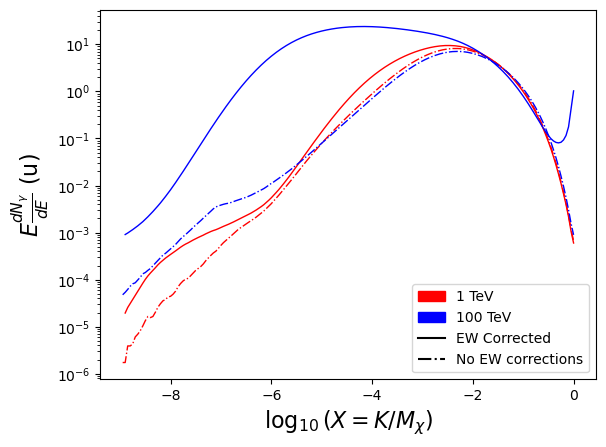
\includegraphics[scale=0.8]{figures/glory_duck/EW_vs_NoEW.png}
}
\caption{Effect of Electroweak (EW) corrections on expected DM annihilation spectrum for $\chi\chi \rightarrow W^-W^+$. Solid lines are spectral models that consider EW corrections. Dash-dot lines are spectral models without EW corrections. Red lines are models for $M_\chi = 1$ TeV. Blue lines represent models for $M_\chi = 100$ TeV. All models are sourced from the PPPC4DMID \cite{Cirelli_2011}.}
\label{fig:ew_vs_noew}
\end{figure}

%%%%%%%%%%%%%%%%%%%%%%%%%%%%%%%%%%%%%%%%%%%%%%%%%%
\subsection{\J - Astrophysical Component}\label{sec:gd_spatialmodel}
%%%%%%%%%%%%%%%%%%%%%%%%%%%%%%%%%%%%%%%%%%%%%%%%%%

The J-factor profiles for each source are imported from Geringer-Sameth (referred to with \GS) \cite{Geringer_Sameth_2015}.
\GS fits the Zhao DM profile to the dSphs which has a DM density described as \cite{Zhao:1995cp}
\zhaoProfile
$R_s$ is the scale radius and free parameter in the model.
$\gamma$ is the logarithmic slope in the region $r << R_s$.
$\beta$ is the logarithmic slope in the region $r >> R_s$.
$\alpha$ is known as the sharpness of transition where $r \approx R_S$.
The classic Navarro-Frenk-White \cite{NFWProfile} (NFW) can be retrieved from Zhao by fixing $(\alpha, \beta, \gamma) = (1,3,1)$.

\GS best fits were pulled from the publication as $\J(\theta)$, where $\theta$ is the angular separation from the center of the source.
HAWC requires maps in terms of $\frac{d\J}{d\Omega}$, so the conversion from the maps was done in the following way...

First, convert the angular distances to solid angles
\angleTOsolidangle
which reduces with a small angle approximation to $\pi \theta^2$.
Next, the central difference for both the $\Delta \J$ and $\Delta \Omega$ value were calculated from the discretized $\J(\theta)$ with the central difference stencil:
\centerDiff
Where $\phi$ is either $\Omega$ or \J.
These were done separately in case the grid spacing in $\theta$~was not uniform.
Finally, these lists are divided so that we are left with an approximation of the $d\J/d\Omega$~profile that is a function of $\theta$.
Admittedly, this is an approximation method for the map which introduces small errors compared to the true profile estimate.
This was checked as a systematic against the author's profiling of the spatial distribution and is documented in \Cref{sec:gd_jfacintegration}.

With $\frac{d\J}{d\Omega}(\theta)$, a map is generated, first by filling in the north-east quadrant of the map.
This quadrant is then reflected twice, vertically then horizontally, to fill the full map.
Maps are then normalized by dividing the discrete 2D integral of the map.
The 2D integral was a simple height of bins, Newton's integral:
\newtonIntegral
These maps are HEALpix maps with NSIDE 16384 and saved in the \texttt{.fits} format.
The hyper fine resolution was selected to better preserve the total expected counts after integrating \cref{eq:id_dm_flux} with the detector response.

\begin{figure}
    \centering{
    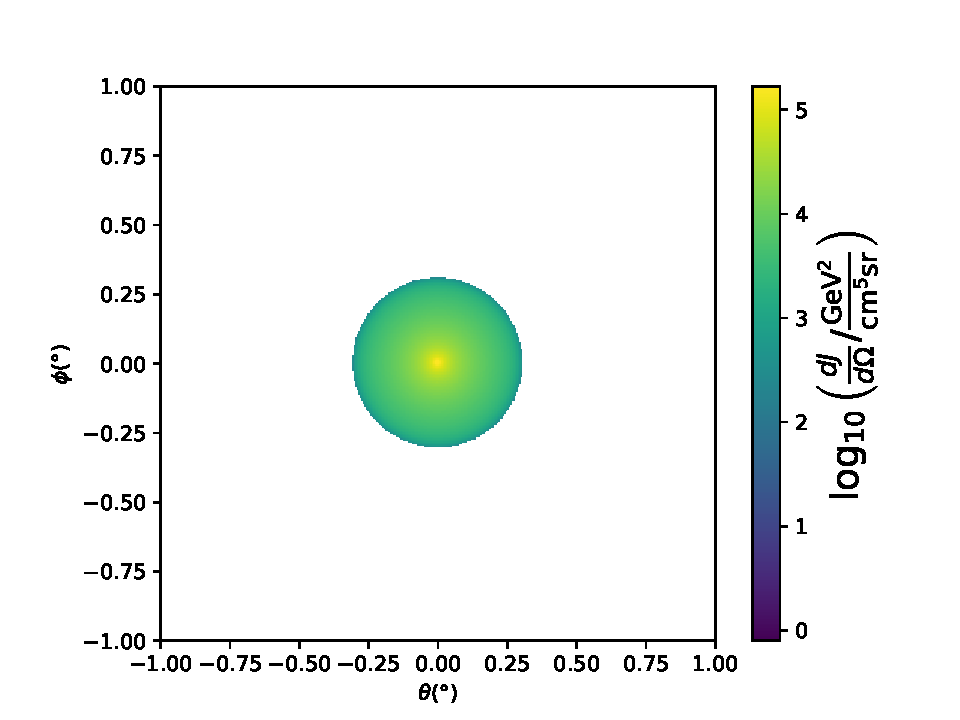
\includegraphics[scale=0.86]{figures/glory_duck/hawc/Segue1_J_plot.pdf}
    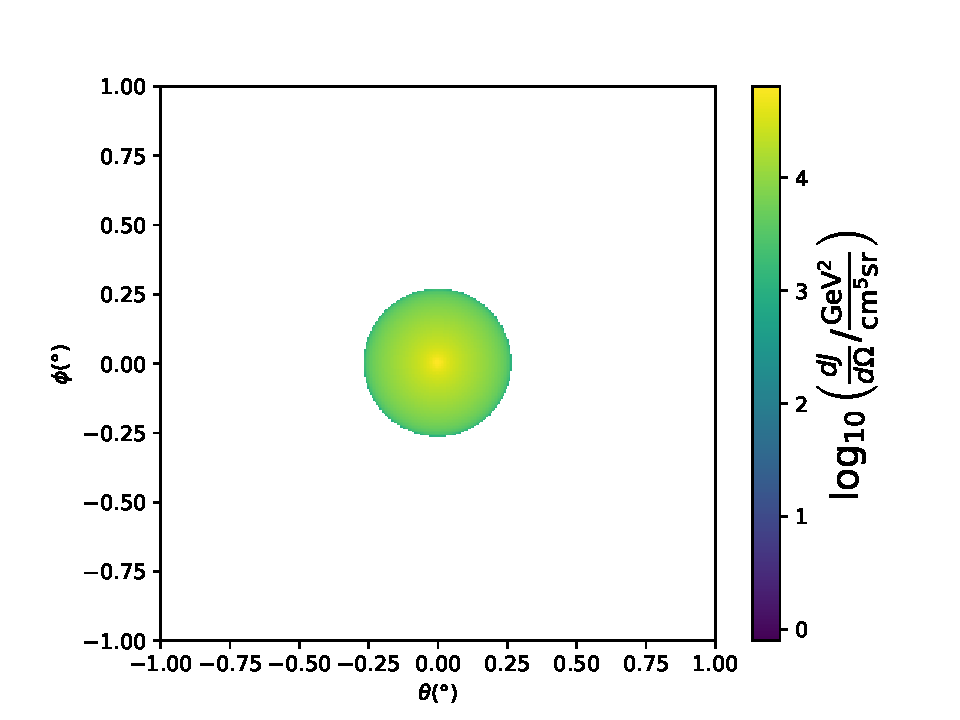
\includegraphics[scale=0.86]{figures/glory_duck/hawc/ComaBerenices_J_plot.pdf}
    }
    \caption{$\frac{d\J}{d\Omega}$ maps for Segue1 (top) and Coma Berenices (bottom). Origin is centered on the specific dwarf spheroidal galaxies (dSph). X and Y axes are the angular separation from the center of the dwarf. Profile is truncated at the scale radius. Plots of the remaining 11 dSph HAWC studied are linked in \cref{fig:apx_gd_spatialmodels}.}\label{fig:gd_spatialmodel}
\end{figure}

Another DM spatial distribution model from Bonnivard (\B) \cite{Bonnivard:2014kza} was used for the Glory Duck study.
However, to save computational time, limits from \GS were scaled to \B instead of each experiment performing a full study a second time.
How these models compare is demonstrated for each dSph in \Cref{fig:comparison_J_1} and \Cref{fig:comparison_J_2}
Plots of these maps are provided for each source in \Cref{apdx:gd_spatial_maps}
Examples of the two most impactful dSphs derived from \GS, Segue1 and Coma Berenices are featured in \Cref{fig:gd_spatialmodel}

%%%%%%%%%%%%%%%%%%%%%%%%%%%%%%%%%%%%%%%%%%%%%%%%%%
\subsection{Source Selection and Annihilation Channels}\label{sec:gd_srcs_y_chan}
%%%%%%%%%%%%%%%%%%%%%%%%%%%%%%%%%%%%%%%%%%%%%%%%%%

We use many of the dSphs presented in HAWC's previous dSph DM search \cite{Albert_2018}.
HAWC's sources for Glory Duck include Boötes I, Coma Berenices, Canes Venatici I + II, Draco, Hercules, Leo I, II, + IV, Segue 1, Sextans, and Ursa Major I + II.
A full description of all sources used in Glory Duck is found in \Cref{tab:gd_J_factor}.
Triangulum II was excluded from the Glory Duck analysis because of large uncertainties in its \J factor.
Ursa Minor was excluded from HAWC's contribution to the combination because the source extension model extended Ursa Minor beyond HAWC's field of view.
Ursa Minor was not expected to contribute significantly to the combined limit, so work was not invested in a solution to include Ursa Minor.

This analysis improves on the previous HAWC dSph paper \cite{Albert_2018} in the following ways.
Previously, the dSphs were treated and implemented as point sources.
For this analysis, dSphs are modeled and treated as extended source.
The impact of this change with respect to the upper limit is source dependent and is explored in \Cref{sec:gd_ext_limitvs_ptsrc}.
Previously, the particle physics model used for gamma-ray spectra from DM annihilation did not have EW corrections where the PPPC includes them.
Finally, the gamma-ray ray dataset is much larger.
The study performed here analyzes over 1000 days of data compared to 507.

The SM annihilation channels probed for the Glory Duck combination include $b\bar{b}$, $e\bar{e}$, $\mu\bar{\mu}$, $\tau\bar{\tau}$, $t\bar{t}$, $W^+W^-$, and $ZZ$.
A summary of all sources, with a description of each experiments' sensitivity to the source, is provided in \Cref{tab:gd_tabSummary}.

\afterpage{%
    \newgeometry{margin=2.5cm} % modify this if you need even more space
    \begin{landscape}
%
\vspace*{\fill}
\begin{table}
\caption{Summary of dSph observations by each experiment used in this work. A `-' indicates the experiment did not observe the dSph for this study. For Fermi-LAT, the exposure at 1~GeV is given. For HAWC, $|\Delta\theta|$ is the absolute difference between the source declination and HAWC latitude. HAWC is more sensitive to sources with smaller $|\Delta\theta|$. For IACTs, we show the zenith angle range, the total exposure, the energy range, the angular radius $\theta$  of the signal or ON region, the ratio of exposures between the background-control (OFF) and signal (ON) regions ($\tau$), and the significance of gamma-ray excess in standard deviations, $\sigma$.}
\centering
{\begin{tabular}{c ? c ? c ? c c c c c c c }
\hline
\hline
& \multicolumn{1}{c?}{Fermi-LAT}  & \multicolumn{1}{c?}{HAWC} & \multicolumn{7}{c}{H.E.S.S, MAGIC, VERITAS} \\
\hline
Source name & Exposure ($10^{11}$ s m$^2$) & $|\Delta\theta|$ (\degree) & IACT & Zenith (\degree) & Exposure (h) & Energy range (GeV) & $\theta$ (\degree) & $\tau$ & S ($\sigma$) \\
\hline\hline
Bo\"{o}tes I            & $2.6$ & $4.5$ & VERITAS  & $15-30$ & $14.0$ & $100 $-$ 41000$ & $0.10$ & $8.6$ & $-1.0$  \\
Canes Venatici I        & $2.9$ & $14.6$ & $-$ & $-$ & $-$ & $-$ & $-$ & $-$ & $-$  \\
Canes Venatici II       & $2.9$ & $15.3$ & $-$ & $-$ & $-$ & $-$ & $-$ & $-$ & $-$  \\
Carina                  & $3.1$ & $-$ & H.E.S.S. & $27-46$ & $23.7$ & $310 - 70000$ & $0.10$ & $18.0$ & $-0.3$  \\
\hdashline
\multirow{2}{*}{Coma Berenices}          & \multirow{2}{*}{$2.7$} & \multirow{2}{*}{$4.9$} & H.E.S.S. & $47-49$ & $11.4$ & $550 - 70000$ & $0.10$ & $14.4$ & $-0.4$  \\
                                         & & & MAGIC & $5 - 37 $ & $49.5$ & $60 - 10000$ & $0.17$ & $1.0$ & $-$\\
\hdashline
\multirow{2}{*}{Draco}                   & \multirow{2}{*}{$3.8$} & \multirow{2}{*}{$38.1$} & MAGIC & $29 - 45$ & $52.1$ & $70 - 10000$ & $0.22$ & $1.0$ & $-$  \\
                                         & & & VERITAS & $25-40$ & $49.8$ & $120 - 70000$ & $0.10$ & $9.0$ & $-1.0$ \\
\hdashline
Fornax                  & $2.7$ & $-$ & H.E.S.S. & $11-25$ & $6.8$ & $230 - 70000$ & $0.10$ & $45.5$ & $-1.5$ \\
Hercules                & $2.8$ & $6.3$ & $-$ & $-$ & $-$ & $-$ & $-$ & $-$ & $-$  \\
Leo I                   & $2.5$ & $6.7$ & $-$ & $-$ & $-$ & $-$ & $-$ & $-$ & $-$  \\
Leo II                  & $2.6$ & $3.1$ & $-$ & $-$ & $-$ & $-$ & $-$ & $-$ & $-$  \\
Leo IV                  & $2.4$ & $19.5$ & $-$ & $-$ & $-$ & $-$ & $-$ & $-$ & $-$ \\
Leo V                   & $2.4$ & $-$ & $-$ & $-$ & $-$ & $-$ & $-$ & $-$ & $-$  \\
Leo T                   & $2.6$ & $-$ & $-$ & $-$ & $-$ & $-$ & $-$ & $-$ & $-$  \\
Sculptor                & $2.7$ & $-$ & H.E.S.S. & $10-46$ & $11.8$ & $200 - 70000$ & $0.10$ & $19.8$ & $-2.2$  \\
\hdashline
\multirow{2}{*}{Segue I}& \multirow{2}{*}{$2.5$} & \multirow{2}{*}{$2.9$} & MAGIC & $13-37$ & $158.0$ & $60 - 10000$ & $0.12$ & $1.0$ & $-0.5$ \\
                        & & & VERITAS & $15-35$ & $92.0$ & $80 - 50000$ & $0.10$ & $7.6$ & $0.7$ \\
\hdashline
Segue II                & $2.7$ & $-$ & $-$ & $-$ & $-$ & $-$ & $-$ & $-$ & $-$ \\
Sextans                 & $2.4$ & $20.6$ & $-$ & $-$ & $-$ & $-$ & $-$ & $-$ & $-$  \\
Ursa Major I            & $3.4$ & $32.9$ & $-$ & $-$ & $-$ & $-$ & $-$ & $-$ & $-$  \\
Ursa Major II           & $4.0$ & $44.1$ & MAGIC & $35-45$ & $94.8$ & $120 - 10000$ & $0.30$ & $1.0$ & $-2.1$  \\
Ursa Minor              & $4.1$ & $-$ &  VERITAS & $35-45$ & 60.4 & $160-93000$ & 0.10 & 8.4 & $-0.1$ \\
\hline
\end{tabular}}
\label{tab:tabSummary}
\end{table}
\vspace*{\fill}
%
\end{landscape}
\restoregeometry
}
%

\begin{table}[h!]
% \captionsetup{font=small}
\centering
    \caption{Summary of the relevant properties of the dSphs used in the present work. Column 1 lists the dSphs. Columns 2 and 3 present their heliocentric distance and galactic coordinates, respectively. Columns 4 and 5 report the \J-factors of each source given from the \GS and \B independent studies and their estimated $\pm 1\sigma$ uncertainties. The values $\log_{10}J$~(\GS set) \cite{Geringer_Sameth_2015} correspond to the mean \J-factor values  for a source extension truncated at the outermost observed star. The values $\log_{10}J$~(\B set) \cite{Bonnivard:2014kza} are provided for a source extension at the tidal radius of each dSph. \textbf{Bolded sources are within HAWC's field of view and provided to the Glory Duck analysis.}}
    {\begin{tabular}{ccccc}
    \hline
    \hline
    \CellTopTwo{}
    Name & Distance & $l, b$ & $\log_{10}J$~(\GS set) & $\log_{10}J$~(\B set)\\
    & \scriptsize{(kpc)} &  \scriptsize{($\degree$)} & \scriptsize{$\log_{10}(\mathrm{GeV}^2 \mathrm{cm}^{-5}\mathrm{sr})$} & \scriptsize{$\log_{10}(\mathrm{GeV}^2 \mathrm{cm}^{-5}\mathrm{sr})$}  \\
    \hline
    \CellTopTwo{}
    \textbf{Bo\"otes} I & $66$ & $358.08,\: 69.62$ & $18.24^{+0.40}_{-0.37}$ & $18.85^{+1.10}_{-0.61}$  \\
    \CellTopTwo{}
    \textbf{Canes Venatici I} & $218$ & $74.31,\: 79.82$ & $17.44^{+0.37}_{-0.28}$ & $17.63^{+0.50}_{-0.20}$  \\
    \CellTopTwo{}
    \textbf{Canes Venatici II} & $160$ & $113.58,\: 82.70$ & $17.65^{+0.45}_{-0.43}$ & $18.67^{+1.54}_{-0.97}$  \\
    \CellTopTwo{}
    Carina & $105$ & $260.11,\: -22.22$ & $17.92^{+0.19}_{-0.11}$ & $18.02^{+0.36}_{-0.15}$ \\
    \CellTopTwo{}
    \textbf{Coma Berenices} & $44$ & $241.89,\: 83.61$ & $19.02^{+0.37}_{-0.41}$ & $20.13^{+1.56}_{-1.08}$  \\
    \CellTopTwo{}
    \textbf{Draco} & $76$ & $86.37,\: 34.72$ & $19.05^{+0.22}_{-0.21}$ &  $19.42^{+0.92}_{-0.47}$  \\
    \CellTopTwo{}
    Fornax & $147$ & $237.10,\: -65.65$ & $17.84^{+0.11}_{-0.06}$ &  $17.85^{+0.11}_{-0.08}$  \\
    \CellTopTwo{}
    \textbf{Hercules} & $132$ & $28.73,\: 36.87$ & $16.86^{+0.74}_{-0.68}$ &  $17.70^{+1.08}_{-0.73}$  \\
    \CellTopTwo{}
    \textbf{Leo I} & $254$ & $225.99,\: 49.11$ & $17.84^{+0.20}_{-0.16}$ &  $17.93^{+0.65}_{-0.25}$  \\
    \CellTopTwo{}
    \textbf{Leo II} & $233$ & $220.17,\: 67.23$ & $17.97^{+0.20}_{-0.18}$ &  $18.11^{+0.71}_{-0.25}$  \\
    \CellTopTwo{}
    \textbf{Leo IV} & $154$ & $265.44,\: 56.51$ & $16.32^{+1.06}_{-1.70}$ & $16.36^{+1.44}_{-1.65}$  \\
    \CellTopTwo{}
    Leo V & $178$ & $261.86,\: 58.54$ & $16.37^{+0.94}_{-0.87}$ & $16.30^{+1.33}_{-1.16}$  \\
    \CellTopTwo{}
    Leo T & $417$ & $214.85,\: 43.66$ & $17.11^{+0.44}_{-0.39}$ & $17.67^{+1.01}_{-0.56}$  \\
    \CellTopTwo{}
    Sculptor & $86$ & $287.53,\: -83.16$ & $18.57^{+0.07}_{-0.05}$ &  $18.63^{+0.14}_{-0.08}$  \\
    \CellTopTwo{}
    \textbf{Segue I} & $23$ & $220.48,\: 50.43$ & $19.36^{+0.32}_{-0.35}$ &  $17.52^{+2.54}_{-2.65}$  \\
    \CellTopTwo{}
    Segue II & $35$ & $149.43,\: -38.14$ & $16.21^{+1.06}_{-0.98}$ & $19.50^{+1.82}_{-1.48}$  \\
    \CellTopTwo{}
    \textbf{Sextans} & $86$ & $243.50,\: 42.27$ & $17.92^{+0.35}_{-0.29}$ &  $18.04^{+0.50}_{-0.28}$  \\
    \CellTopTwo{}
    \textbf{Ursa Major I} & $97$ & $159.43,\: 54.41$ & $17.87^{+0.56}_{-0.33}$ & $18.84^{+0.97}_{-0.43}$  \\
    \CellTopTwo{}
    \textbf{Ursa Major II} & $32$ & $152.46,\: 37.44$ & $19.42^{+0.44}_{-0.42}$ & $20.60^{+1.46}_{-0.95}$  \\
    \CellTopTwo{}
    Ursa Minor & $76$ & $104.97,\: 44.80$ & $18.95^{+0.26}_{-0.18}$ & $19.08^{+0.21}_{-0.13}$  \\
    \hline
    \hline
    \CellTopTwo{}
\end{tabular}} \label{tab:gd_J_factor}
\end{table}

%%%%%%%%%%%%%%%%%%%%%%%%%%%%%%%%%%%%%%%%%%%%%%%%%%%%%%%%%%%%%
\section{Likelihood Methods} \label{sec:gd_ll_methods}
%%%%%%%%%%%%%%%%%%%%%%%%%%%%%%%%%%%%%%%%%%%%%%%%%%%%%%%%%%%%%

%%%%%%%%%%%%%%%%%%%%%%%%%%%%%%%%%%%%%%%%%%%%%%%%%%%%%%%%%%%%%
\subsection{HAWC Likelihood}\label{sec:gd_hawc_llh}
%%%%%%%%%%%%%%%%%%%%%%%%%%%%%%%%%%%%%%%%%%%%%%%%%%%%%%%%%%%%%

For every analysis bin in energy, $f_{hit}$ bins (1-9), and location, we can expect $N$ signal events and $B$ background events.
The expected number of excess signal events from dark matter annihilation, $S$, is estimated by convolving \Cref{eq:id_dm_flux} with HAWC's energy response and pixel point spread functions.
I then compute the test statistic (TS) with the log-likelihood ratio test,
\gdTS
where $\mathcal{L}_0$~is the null hypothesis, or no DM emission, likelihood.
$\mathcal{L}^\mathrm{max}$~is the best fit signal hypothesis where \sv~maximizes the likelihood.
We calculate the likelihood of each source and model, assuming events are Poisson distributed, with
\hwcpsLLH
where $S_i$ is the sum of expected number of signal counts.
$B_i$ is the number of background counts observed.
$N_i$ is the total number of counts.

I also calculate an upper limit on \sv~ by calculating the $95\%$ confidence level (CL).
For the CL, we define a parameter, $TS_{95}$, as
\gdHAWCCL
where the expected signal counts from a dSph is scaled by $\epsilon$.
$S_\mathrm{ref}$ is the expected number of excess counts in a bin from DM emission from a dSph with a corresponding annihilation cross-section, \sv.
We scan $\epsilon$ such that
\CLbyTS
HAWC's exclusive results are provided in \cref{sec:hawc_results}.

%%%%%%%%%%%%%%%%%%%%%%%%%%%%%%%%%%%%%%%%%%%%%%%%%%%%%%%%%%%%%
\subsection{Glory Duck Joint Likelihood}\label{sec:gd_joint_llh}
%%%%%%%%%%%%%%%%%%%%%%%%%%%%%%%%%%%%%%%%%%%%%%%%%%%%%%%%%%%%%

The joint likelihood for the 5-experiment combination was done similarly as \Cref{sec:gd_hawc_llh}.
We calculate upper limits on \sv~from the TS, \cref{eq:gd_TS}, and define the likelihood ratio more generally
\gdLHratio
$\bm{\mathcal{D}_{\mathrm{dSphs}}}$ is the totality of observations across experiments and dSphs.
$\bm{\nu}$ are the nuisance parameters which are the \J factors in this study.
$\widehat{\svtex}$ and $\hat{\bm{\nu}}$ are the respective estimate that maximize $\mathcal{L}$ globally.
Finally, $\hat{\hat{\bm{\nu}}}$ is the set of nuisance parameters that maximize $\mathcal{L}$ for a fixed value of \sv.

The \textit{complete} joint likelihood, $\mathcal{L}$ that encompasses all observations from all instruments and dSphs can be factorized into \textit{partial} functions for each dSph $l$ (with $\mathcal{L}_{\mathrm{dSph}, l}$) and its \J factor ($\mathcal{J}_l$):
\CompleteGDLLH
For this study, $N_{\mathrm{dSphs}}=20$ is the number of dSphs studied.
$\bm{\mathcal{D}_{l}}$ are the gamma-ray observations of dSph, $l$.
$\bm{\nu_l}$ are the nuisance parameters modifying the gamma-ray observations of dSph, $l$, but excludes $\mathcal{J}_l$.
$\mathcal{J}_l$ is the \J factor for dSph, $l$, as defined in \Cref{eq:jfactor}, and it is a nuisance parameter whose value is unknown.
$\log_{10} J_{l,\mathrm{obs}}$ and $\sigma_{\log{J_l}}$ are obtained by fitting a log-normal function of $J_{l,\mathrm{obs}}$ to the posterior distribution of $J_{l}$~\cite{2015PhRvL.115w1301A}.
$\log_{10} J_{l,\mathrm{obs}}$ and $\sigma_{\log{J_l}}$ values are provided in \Cref{tab:gd_J_factor}.
The term $\mathcal{J}_l$ constraining $J_l$ is written as:
\JLgdLLH
Both the \GS and \B, displayed in \Cref{tab:gd_J_factor}, sets of \J factors are used in this analysis.
\Cref{eq:J_lkl} is also normalized, so it can also be interpreted as a probability density function (PDF) for $J_{l,\mathrm{obs}}$.
From \Cref{eq:id_dm_flux}, we can also see that \sv~and $\J_l$ are degenerate when computing $\mathcal{L}_{\mathrm{dSph},l}$.
Therefore, as noted in~\cite{MAGICFermi_combo}, it is sufficient to compute $\mathcal{L}_{\mathrm{dSph},l}$ versus \sv~for a fixed value of $J_{l}$.
We used $J_{l,\mathrm{obs}}$(\GS) reported in \cref{tab:gd_J_factor}, in order to perform the profile of $\mathcal{L}$ with respect to $J_l$.
The degeneracy implies that for any $J'_l \neq J_{l,\mathrm{obs}}$ (in practice in our case we used $J'_l = J_{l,\mathrm{obs}}$(\B) to compute results from a different set of \J factors):
\jfacTrick
which is a straightforward rescaling operation that reduces the computational needs of the profiling operation since:
\rescaleTrick
In addition, \cref{eq:Jfactor_trick} enables the combination of data from different gamma-ray instruments and observed dSphs via tabulated values of $\mathcal{L}_{\mathrm{dSph},l}$, or equivalently of $\lambda$ from~\cref{eq:gd_LLH_test} as was done in this work, versus \sv.
$\mathcal{L}_{\mathrm{dSph},l}$ is computed for a fixed value of $\J_l$ and profiled with respect to all instrumental nuisance parameters $\bm{\nu_l}$, these nuisance parameters are discussed in more detail below.
These values are produced by each detector independently and therefore there is no need to share sensitive low-level information used to produce them, such as event lists.
\Cref{fig:illustration_combination} illustrates the multi-instrument combination technique used in this study with a comparison of the upper limit on \sv~obtained from the combination of the observations of four experiments towards one dSph versus the upper limit from individual instruments.
It also shows graphically the effect of the \J-factor uncertainty on the combined observations.

\begin{figure}[t]
    \centering{
    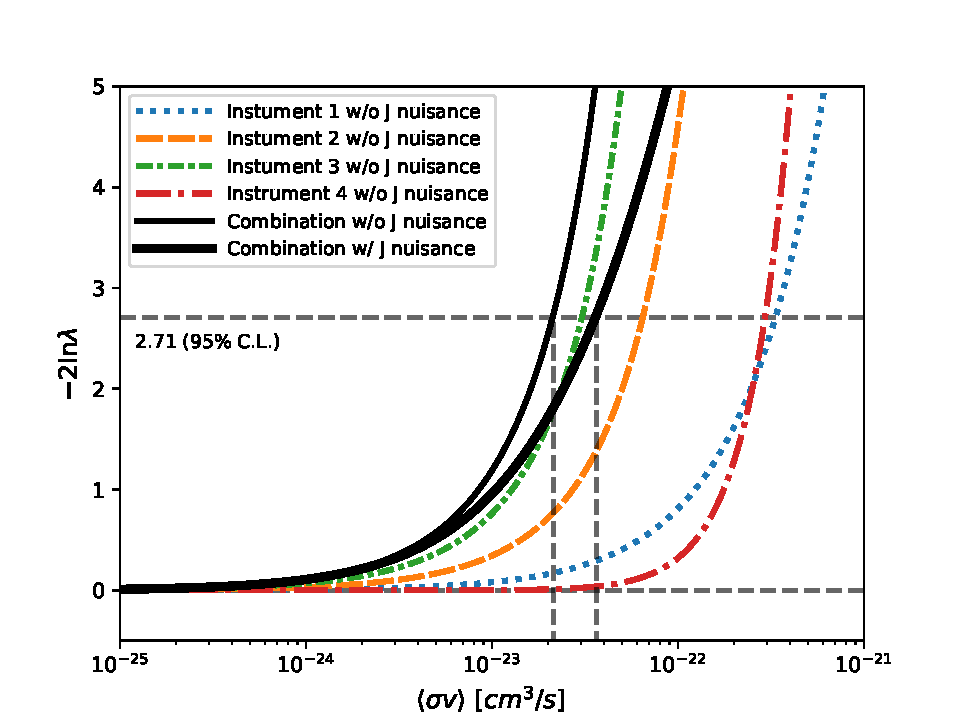
\includegraphics[width=0.7\textwidth]{figures/glory_duck/comparison/Combined_exp_technique_20TeV_4exp_J_with_without_nuisance_v2.pdf}
    }
    \caption{Illustration of the combination technique showing a comparison between $-2\ln  \lambda$ provided by four instruments (colored lines) from the observation of the same dSph without any \J nuisance and their sum, $i.e.$ the resulting combined likelihood (thin black line). According to the test statistics of \Cref{eq:gd_TS}, the intersection of the likelihood profiles with the line $-2\ln  \lambda$ = 2.71 indicates the 95\% C.L. upper limit on \sv. The combined likelihood (thin black line) shows a smaller value of upper limit on \sv than those derived by individual instruments. We also show how the uncertainties on the \J factor effects the combined likelihood and degrade the upper limit on \sv (thick black line). All likelihood profiles are normalized so that the global minimum $\widehat{\svtex}$ is 0. We note that each profile depends on the observational conditions in which a target object was observed. The sensitivity of a given instrument can be degraded and the upper limits less constraining if the observations are performed in non-optimal conditions such as a high zenith angle or a short exposure time.}
    \label{fig:illustration_combination}
\end{figure}

The \textit{partial} joint likelihood function for gamma-ray observations of each dSph ($\mathcal{L}_{\text{dSph},l}$) is written as the product of the likelihood terms describing the $N_{\mathrm{exp},l}$ observations performed with any of our observatories:
\GDjointLLH
where each $\mathcal{L}_{lk}$ term refers to an observation of the $l$-th dSph with associated $k$-th instrument responses.
$ N_{\mathrm{exp},l} $ varies from dSph to dSph and can be inferred from \Cref{tab:gd_tabSummary}.

Each collaboration separately analyzes their data for $\bm{\mathcal{D}_{lk}}$ corresponding to dSph $l$ and gamma-ray detector $k$, using as many common assumptions as possible in the analysis.
HAWC's treatment was described earlier in \Cref{sec:gd_hawc_llh} whereas the specifics of the remaining experiments is left to the publication.
We compute the values for the likelihood functions $\mathcal{L}_{lk}$ (see~\cref{eq:measurement_combination}) for a fixed value of $\J_l$ and profile over the rest of the nuisance parameters $\bm{\nu_{lk}}$.
Then, values of $\lambda$ from \cref{eq:gd_LLH_test} are computed as a function of \sv, and shared using a common format.
Results are computed for seven annihilation channels, $W^+W^-$, $ZZ$, $b\bar{b}$, $t\bar{t}$, $e^+e^-$, $\mu^+\mu^-$, and $\tau^+\tau^-$ over 62 $m_{\chi}$ values between 5 GeV and 100 TeV provided in~\cite{Cirelli_2011}.
The \sv range is defined between $10^{-28}$ and $10^{-18}\mathrm{cm}^{3}\cdot \mathrm{s}^{-1}$, with 1001 logarithmically spaced values.
The likelihood combination, i.e. \Cref{eq:dSph_combination}, and profile over the \J-factor to compute the profile likelihood ratio $\lambda$, \Cref{eq:gd_LLH_test}, are carried out with two different public analysis software packages, namely \texttt{gLike}~\cite{javier_rico_2021_4601451} and \texttt{LklCom}~\cite{tjark_miener_2021_4597500}, that provide the same results~\cite{2021arXiv211201818M}.

As mentioned previously, each experiment computes the $\mathcal{L}_{lk}$ from \Cref{eq:gd_LLH_test} differently.
The remainder of this section highlights the differences in this calculation across the experiments.
Four experiments, namely \textit{Fermi}-LAT, H.E.S.S., HAWC and MAGIC, use a binned likelihood to compute the $\mathcal{L}_{lk}$.
For these experiments, for each observation $\bm{\mathcal{D}_{lk}}$ of a given dSph $l$ carried out using a given gamma-ray detector $k$, the binned likelihood function is:
\gdJointLLH
where $N_{\text{E'}}$ and $N_{\text{P'}}$ are the number of considered bins in reconstructed energy and arrival direction, respectively; $\mathcal{P}$ represents a Poisson PDF for the number of gamma-ray candidate events $ N_{lk,ij} $ observed in the $i$-th bin in energy and $j$-th bin in arrival direction, when the expected number is the sum of the expected mean number of signal events $ s_{ij} $ (produced by DM annihilation) and of background events $ b_{ij} $; $ \mathcal{L}_{lk,\bm{\nu}} $ is the likelihood term for the extra $ \bm{\nu_{lk}} $ nuisance parameters that vary from one instrument $k$ to another.
The expected counts for signal events $s_{ij}$ for a given dSph $l$ and detector $k$ is given by:
\gdExpectedNS
where $ E' $ and $ E $ are the reconstructed and true energies, $ P' $ and $ P $ the reconstructed and true arrival directions; $ E'_{\text{min},i} $, $ P'_{\text{min},j} $, $ E'_{\text{max},i} $, and $ P'_{\text{max},j} $ are their lower and upper limits of the $ i $-th energy bin and the $ j $-th arrival direction bin; $ T_{\text{obs}} $ is the (dead-time corrected) total observation time; $ t $ is the time along the observations; $ \text{d}^{2}\Phi/\text{d}E\text{d}\Omega $ is the DM flux in the source region (see \Cref{eq:id_dm_flux});
and $ \text{IRF} \left( E', P' \mid E, P, t \right) $ is the IRF, which can be factorized as the product of the effective collection area of the detector $ A_{\mathrm{eff}} (E, P, t) $, the PDFs for the energy estimator $ f_{E} (E' \mid E,t) $, and arrival direction $ f_{P} (P' \mid E,P,t) $ estimators.
Note that for Fermi-LAT, HAWC, MAGIC, and VERITAS the effect of the finite angular resolution is taken into account through the convolution of $d\Phi/dE d\Omega$ with $f_{P}$ in \Cref{eq:gd_expected_ns}, whereas in the cases of H.E.S.S. $f_{P}$ is approximated by a delta function.
This approximation has been made in order to maintain compatibility of the result with what has been previously published.
The difference introduced by this approximation is $<5\%$ for all considered dSphs.
A more comprehensive review of the differences between the analyses of different instruments can be found in~\cite{2020Galax...8...25R}.

%%%%%%%%%%%%%%%%%%%%%%%%%%%%%%%%%%%%%%%%%%%%%%%%%%%%%%%%%%%%%
\section{HAWC Results}\label{sec:hawc_results}
%%%%%%%%%%%%%%%%%%%%%%%%%%%%%%%%%%%%%%%%%%%%%%%%%%%%%%%%%%%%%

\begin{figure}[ht]
    \centering{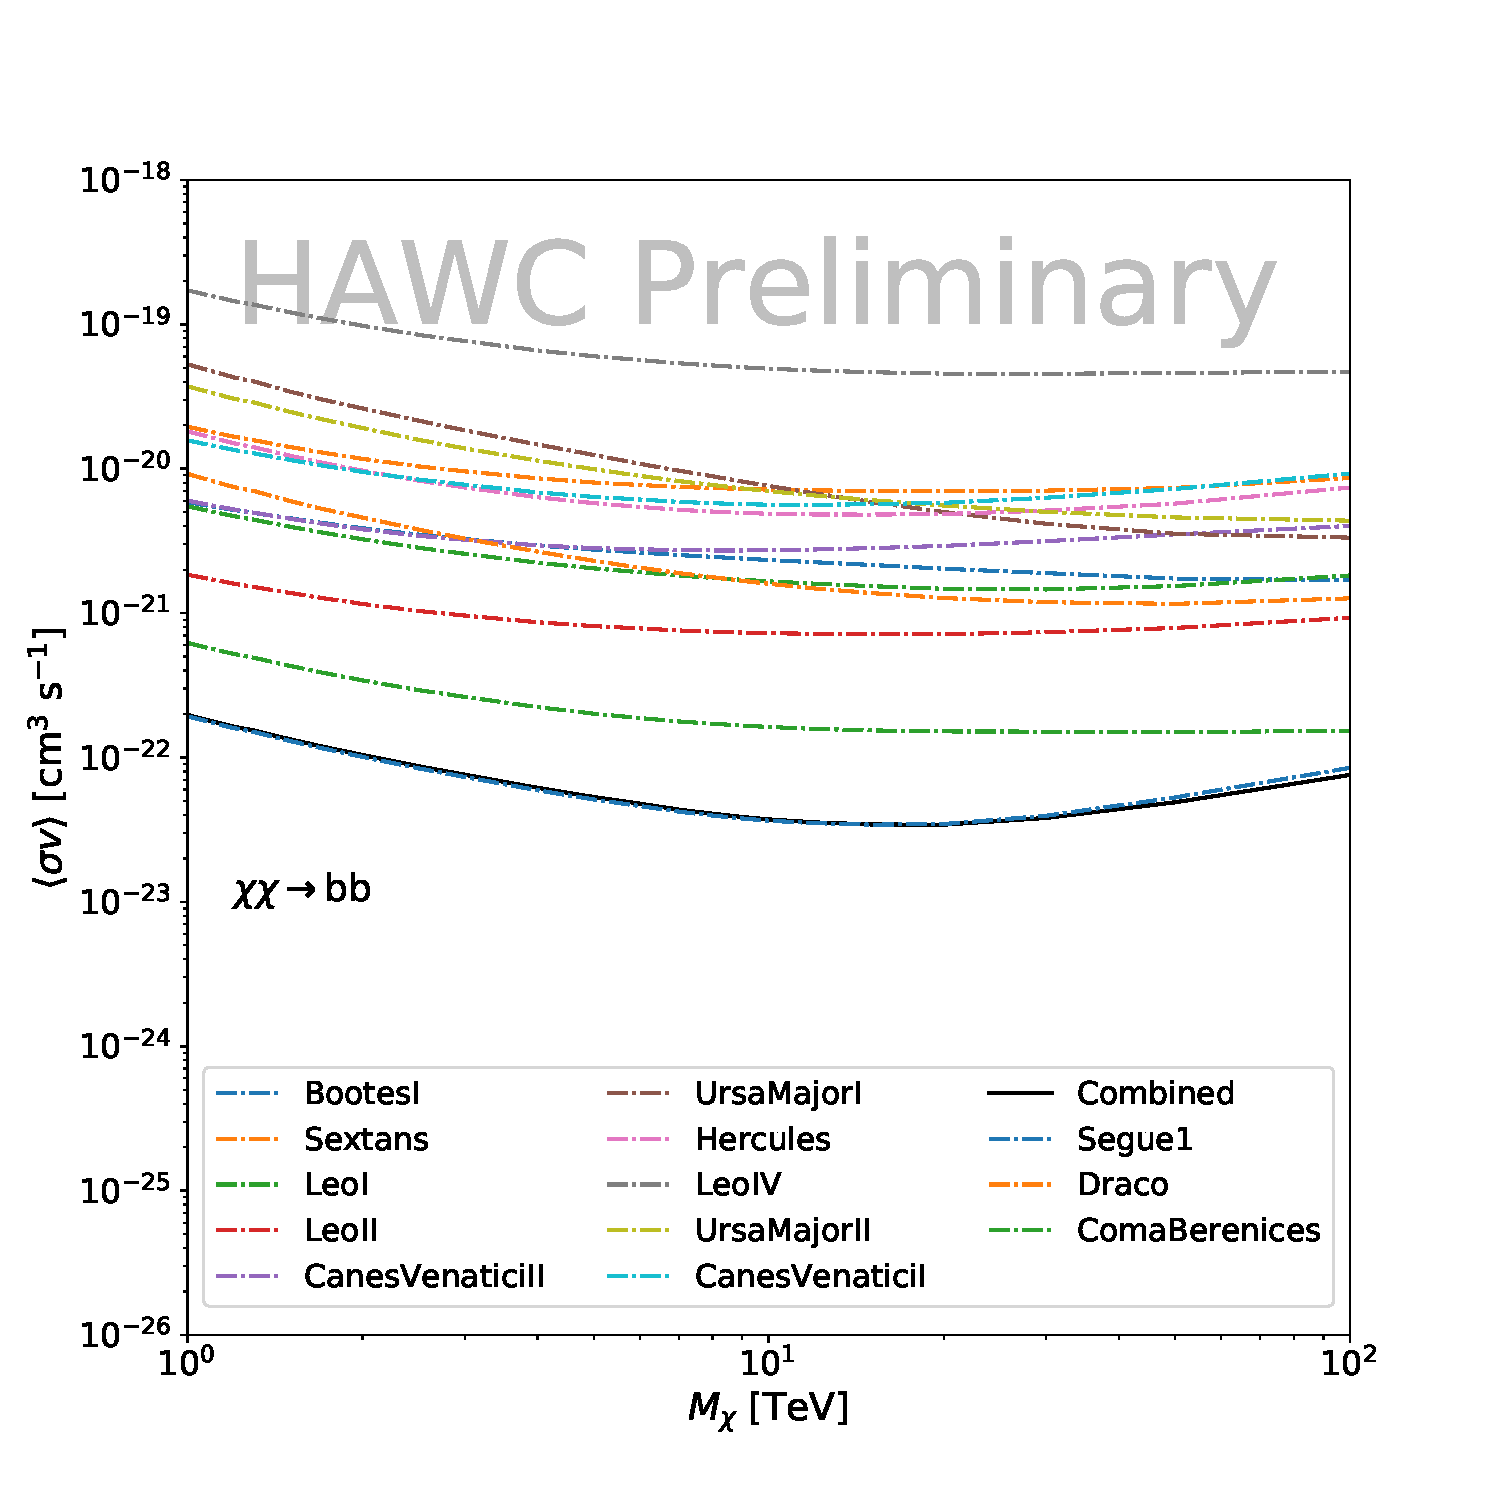
\includegraphics[scale=0.21]{figures/glory_duck/hawc/Combined95_GD_bb.pdf}
    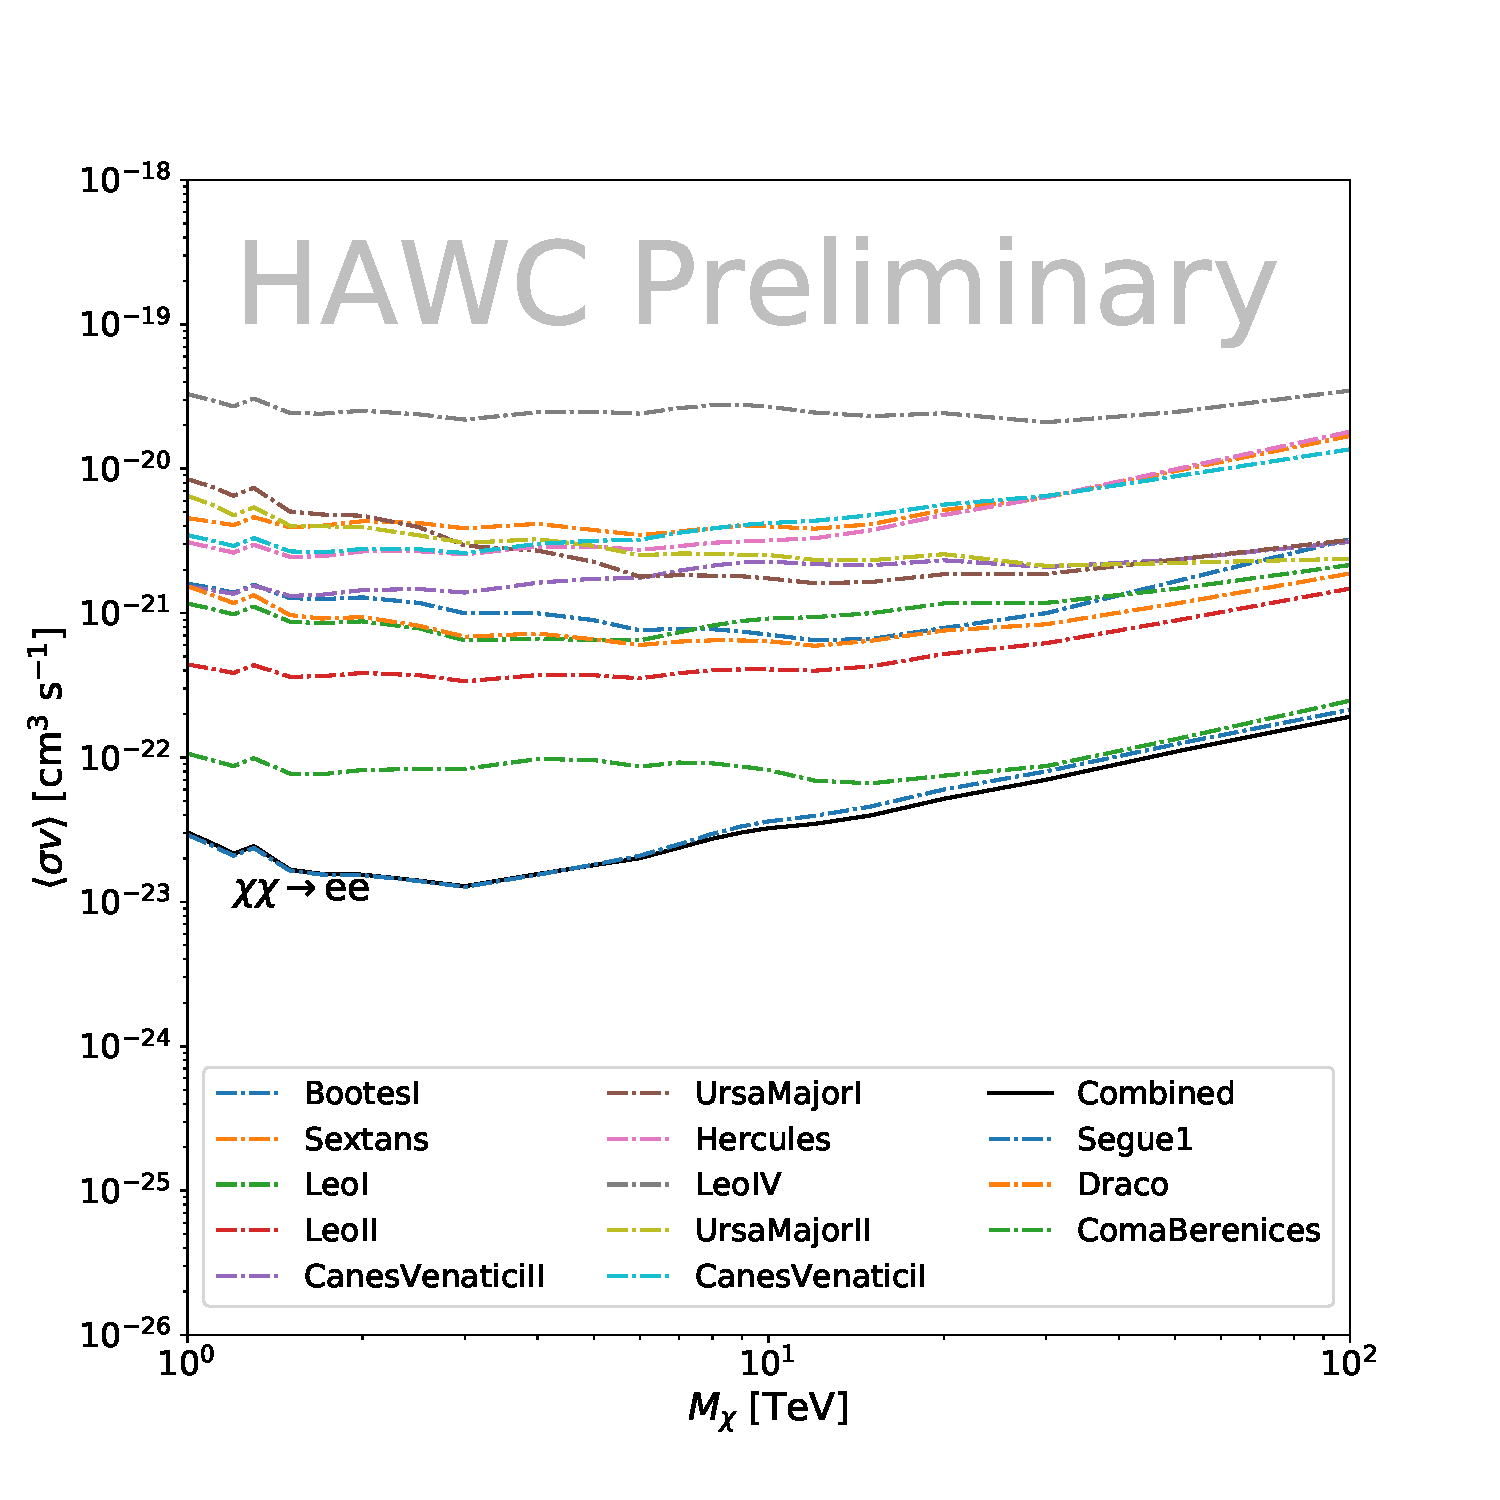
\includegraphics[scale=0.215]{figures/glory_duck/hawc/Combined95_GD_ee.pdf}
    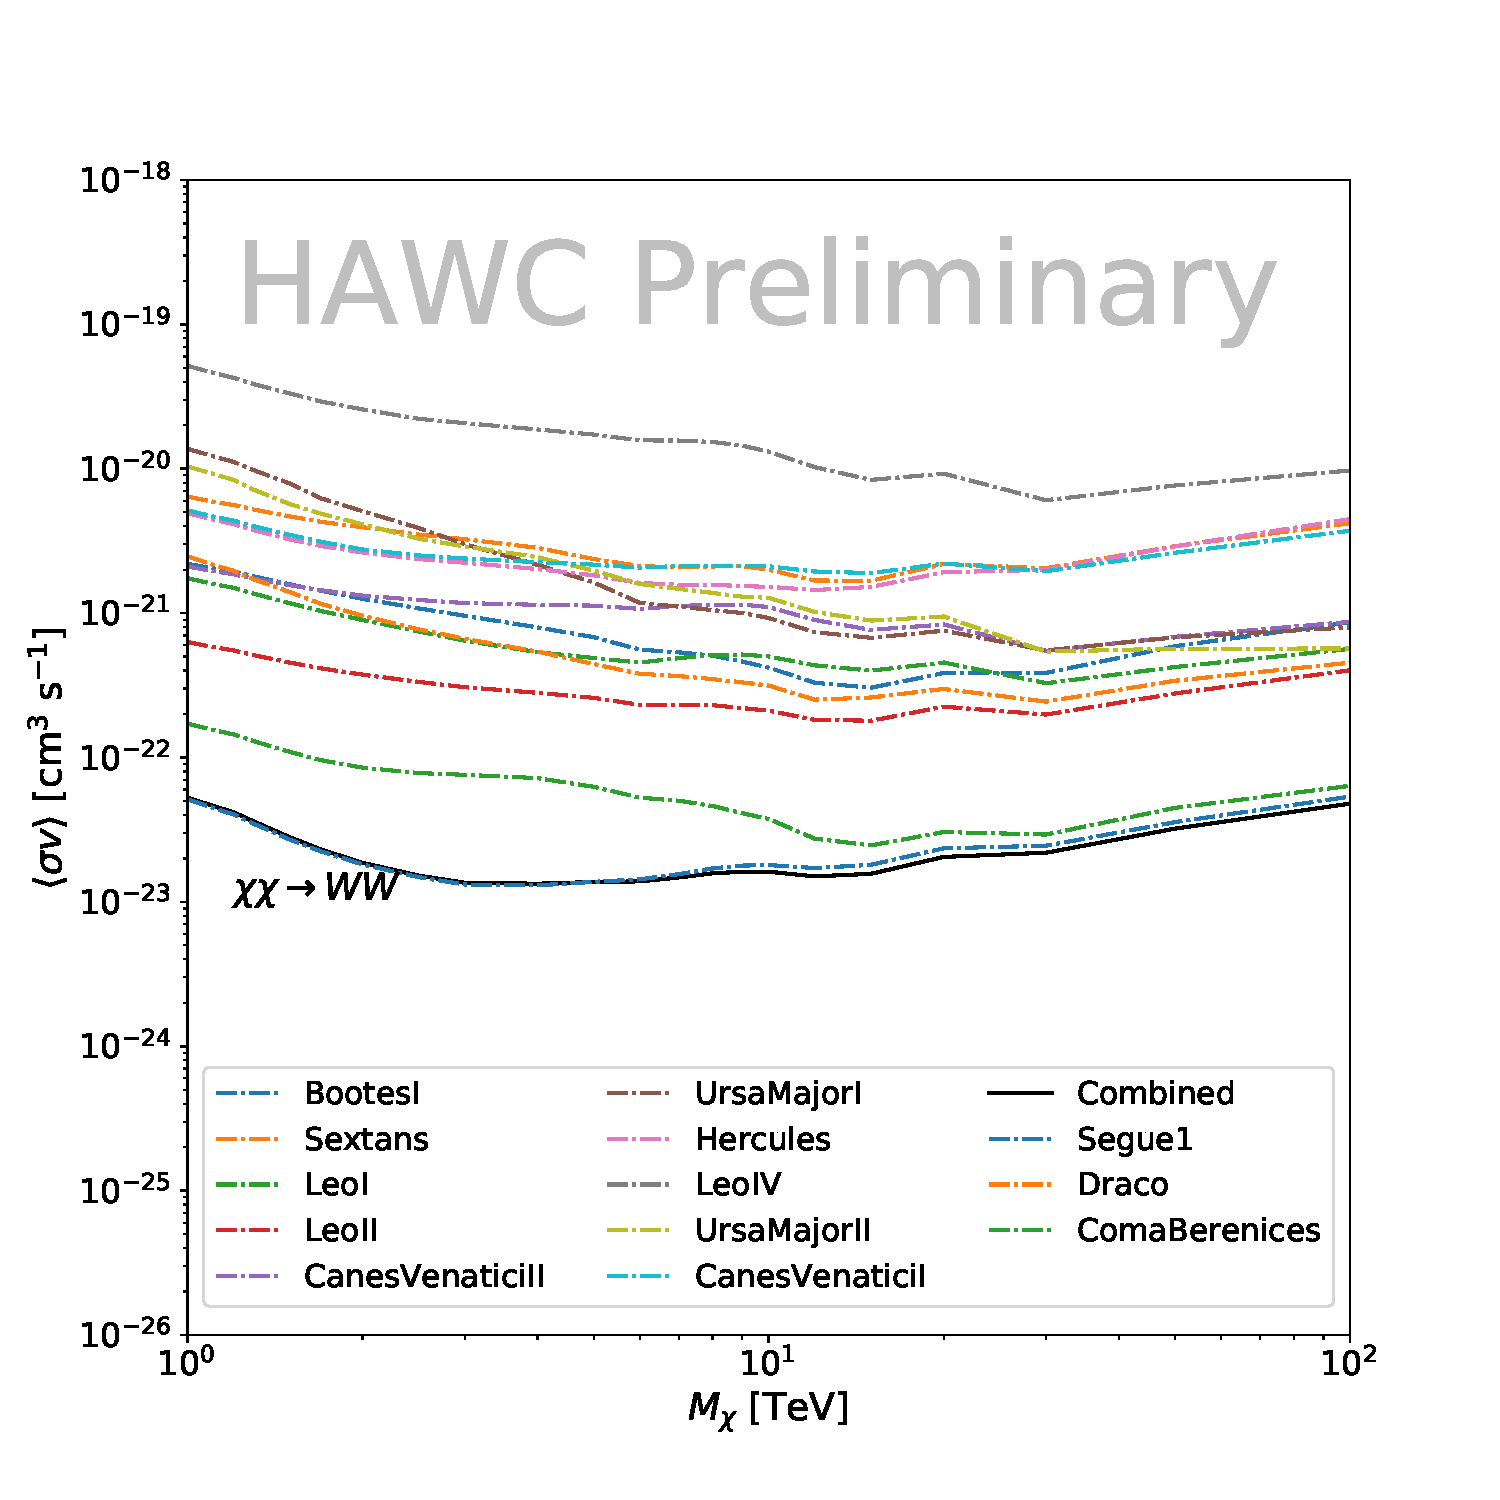
\includegraphics[scale=0.215]{figures/glory_duck/hawc/Combined95_GD_ww.pdf}
    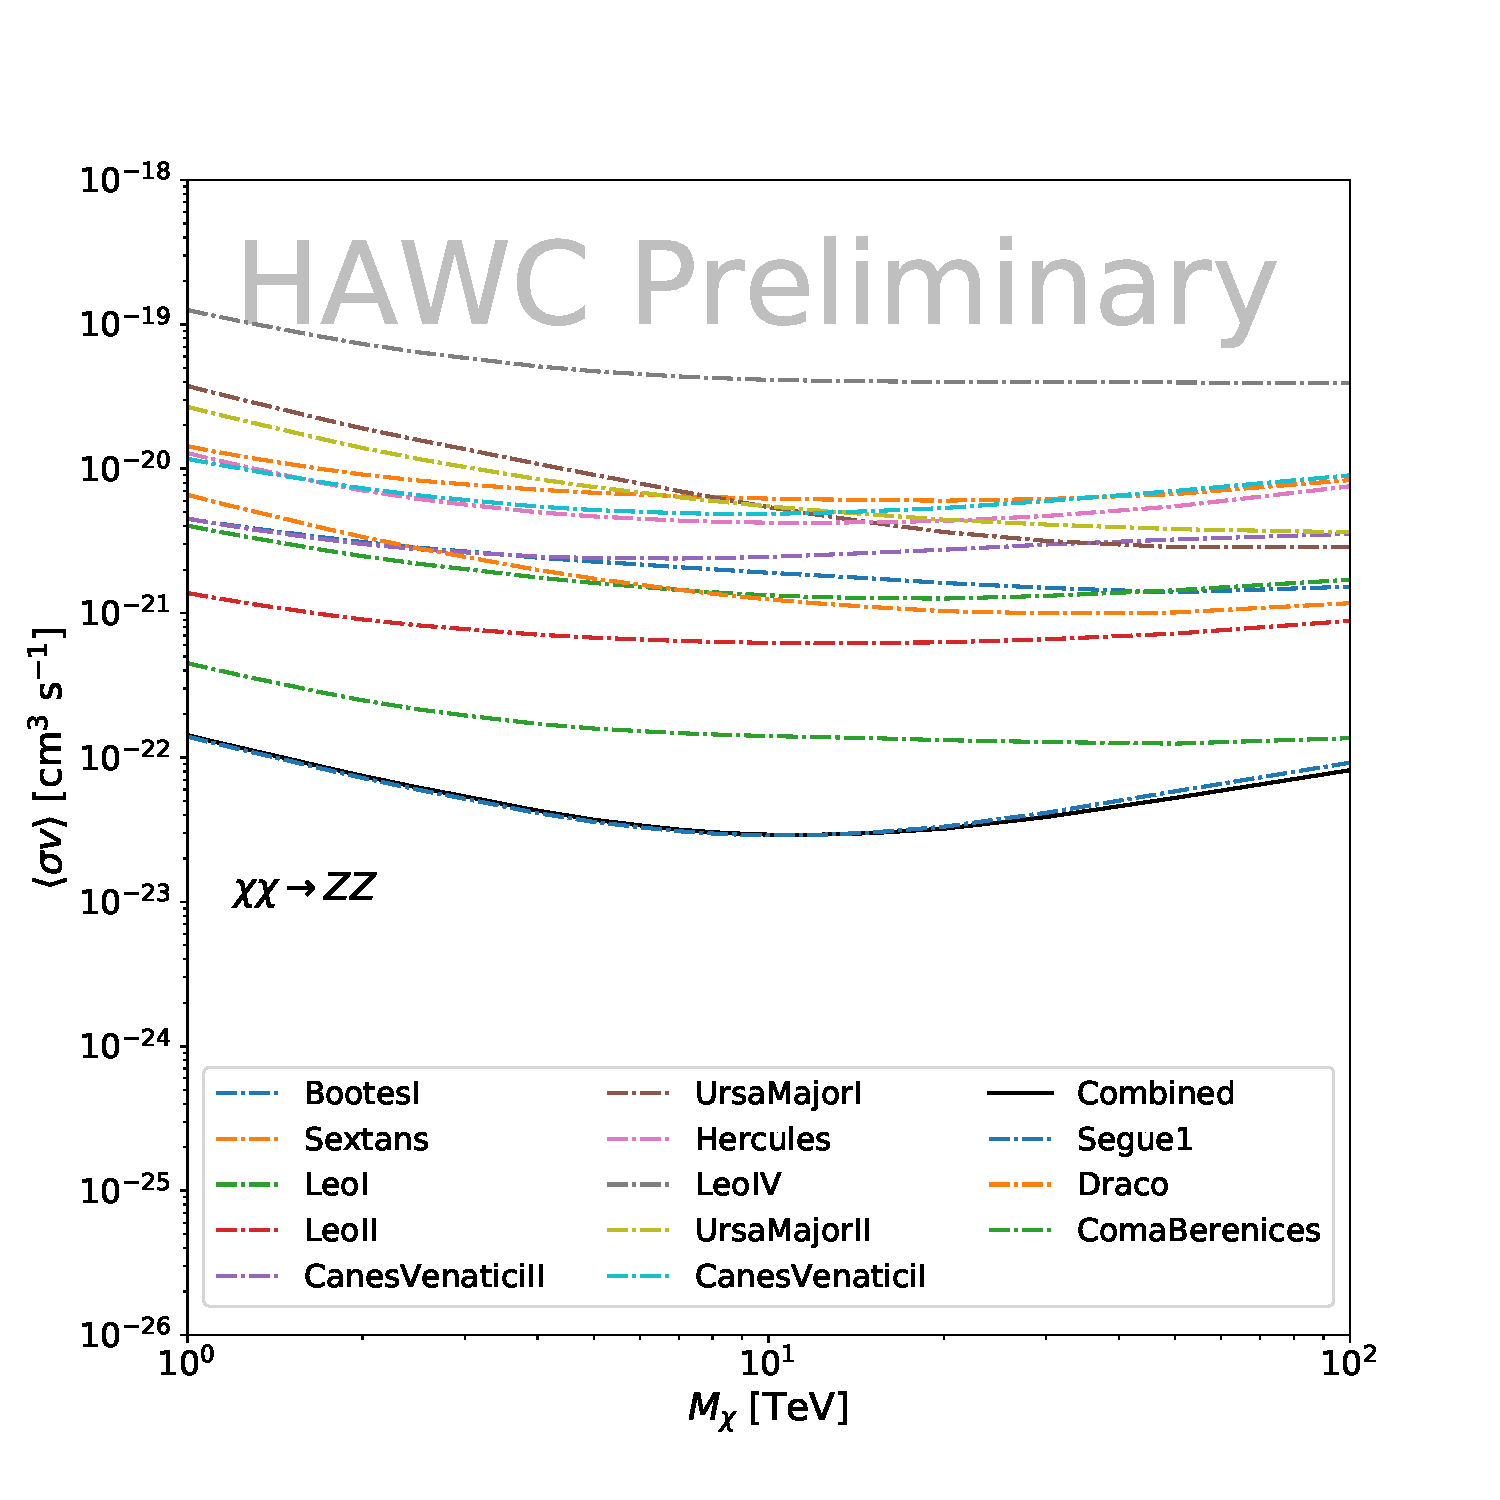
\includegraphics[scale=0.215]{figures/glory_duck/hawc/Combined95_GD_zz.pdf}
    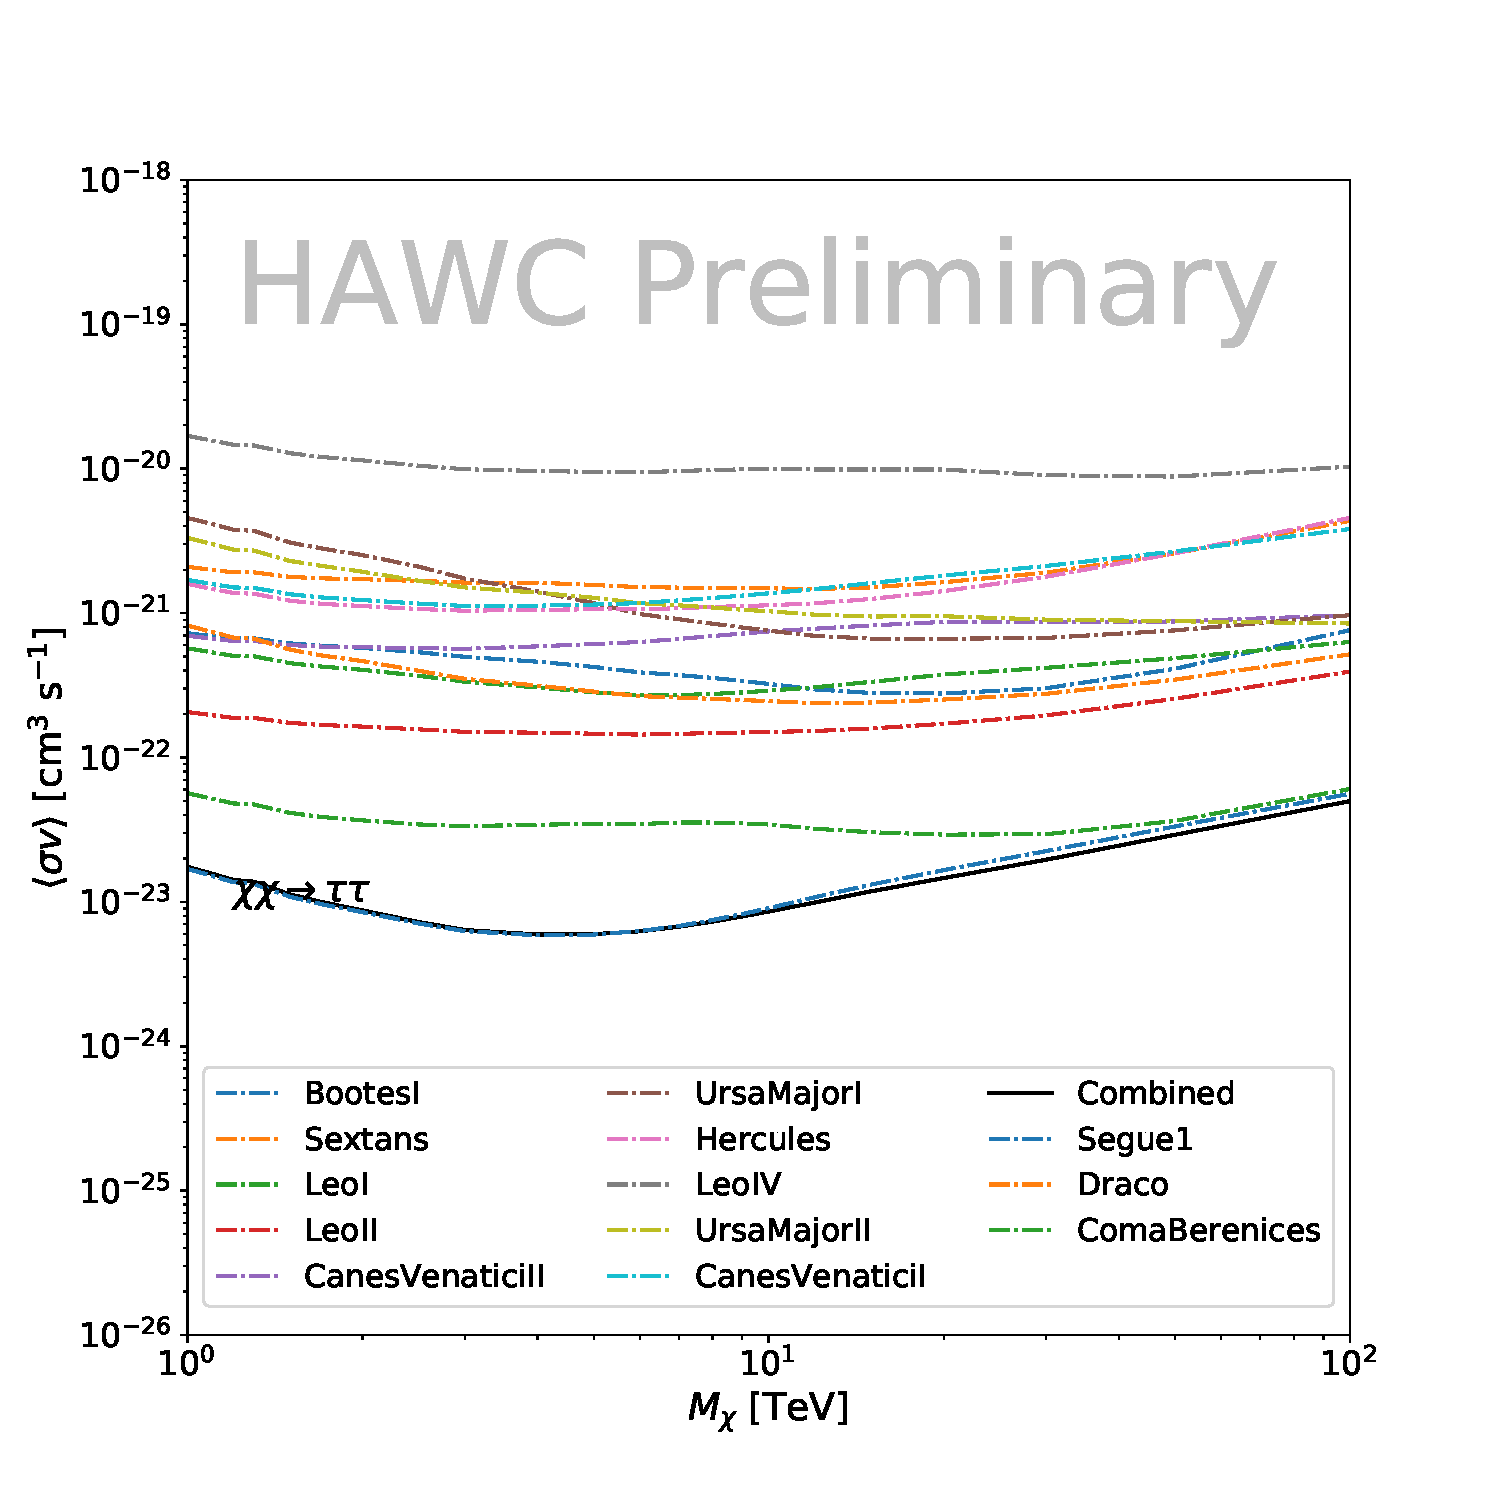
\includegraphics[scale=0.215]{figures/glory_duck/hawc/Combined95_GD_tautau.pdf}
    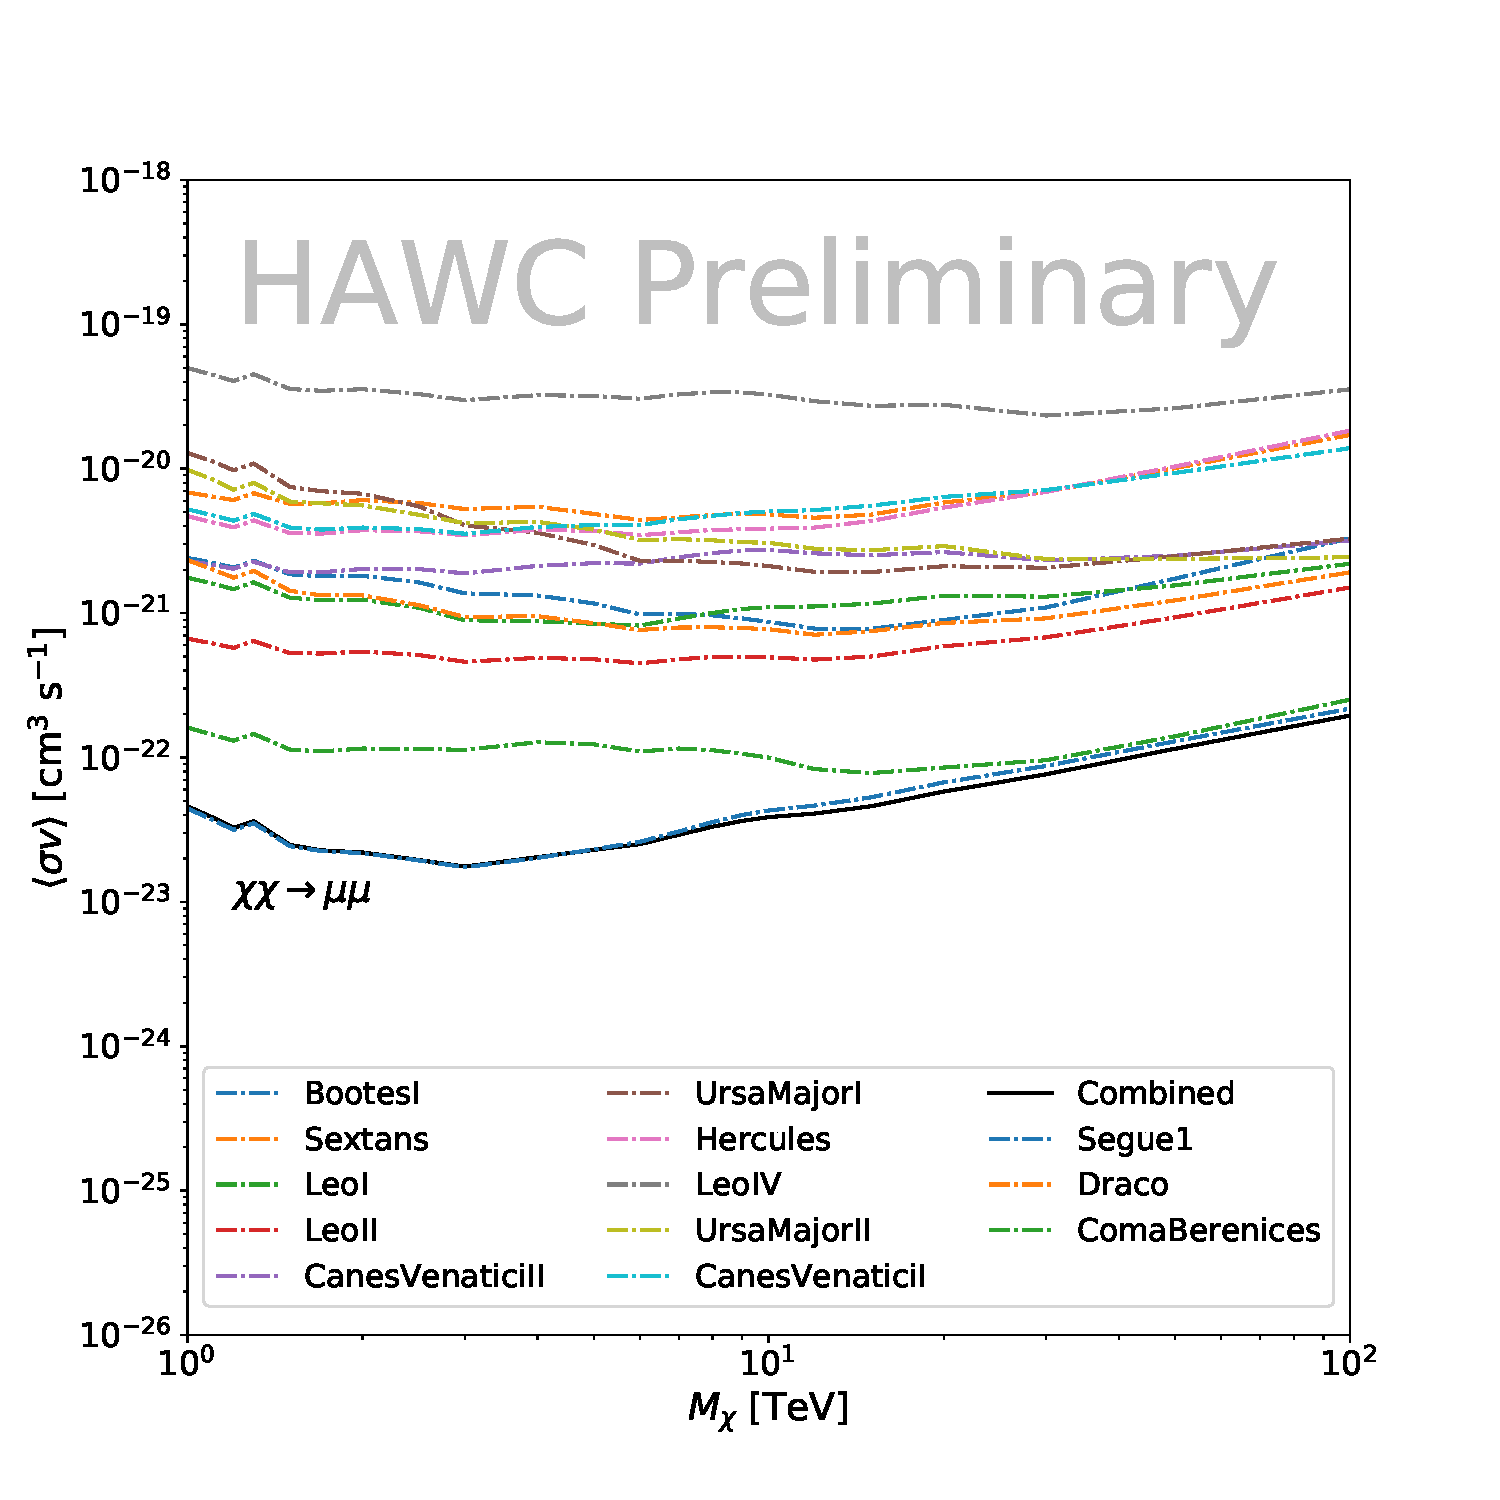
\includegraphics[scale=0.215]{figures/glory_duck/hawc/Combined95_GD_mumu.pdf}
    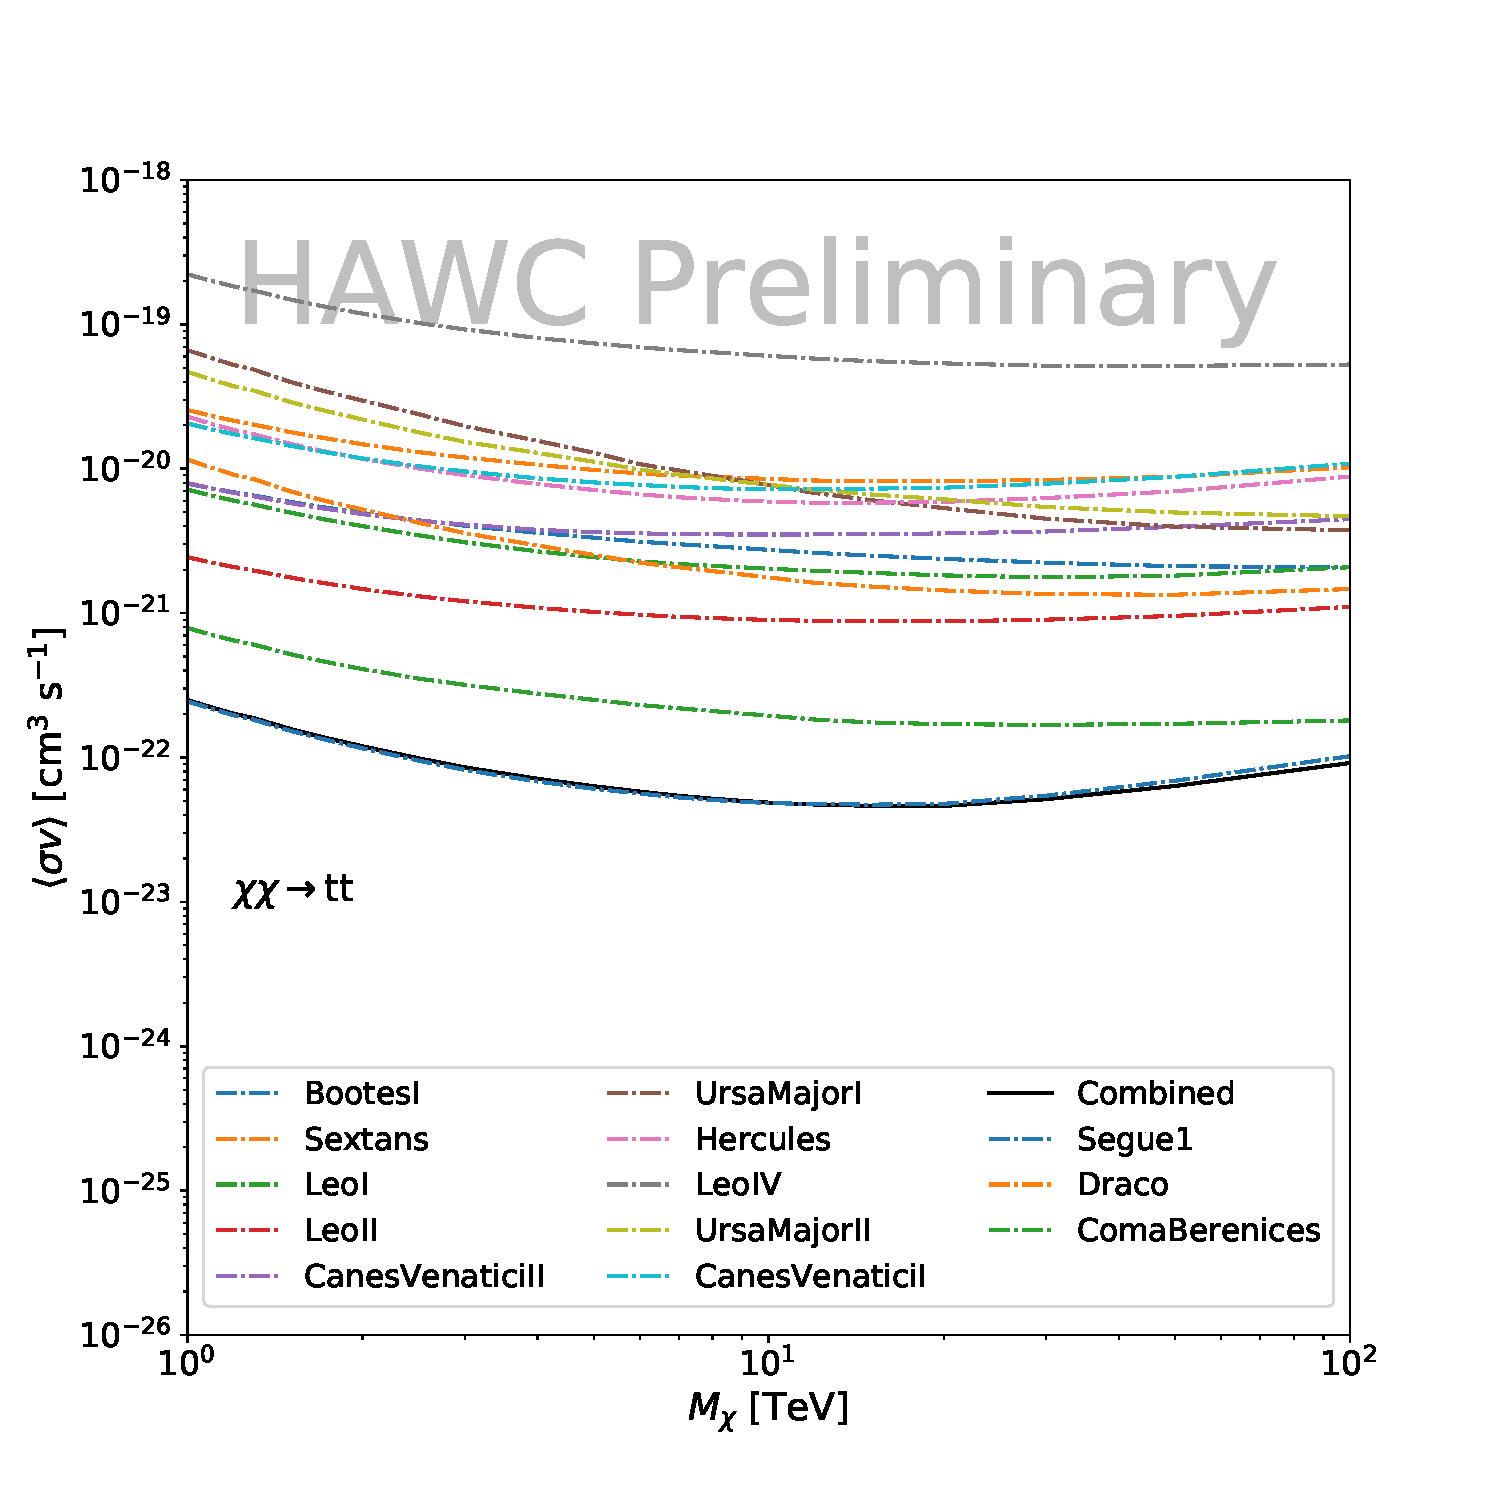
\includegraphics[scale=0.215]{figures/glory_duck/hawc/Combined95_GD_tt.pdf}
    }
    \caption{}
 \label{fig:hawc_combined_limit}
\end{figure}

13 of the 20 dSphs considered for the Glory Duck analysis are within HAWC's field of view.
These dSph are analyzed for emission from DM annihilation according to the likelihood method described in \Cref{sec:gd_ll_methods}.
The 13 likelihood profiles are then stacked to synthesize a combined limit on the dark matter cross-section, \sv.
This combination is done for the 7 SM annihilation channels used in the Glory Duck analysis.
\Cref{fig:hawc_combined_limit} shows the combined limit for all annihilation channels with HAWC only observations.
We also perform 300 studies of Poisson trials on the background.
These trials are used to produce HAWC sensitivities with $\pm1\sigma$ and $\pm2\sigma$ uncertainty bands which were shared with the other collaborators for combination.
The results on fitting to HAWC's Poisson trials of the DM hypothesis is shown in \Cref{fig:hawc_brazil_band} for all the DM annihilation channels studied for Glory Duck.

\begin{figure}[t]
    \centering{
        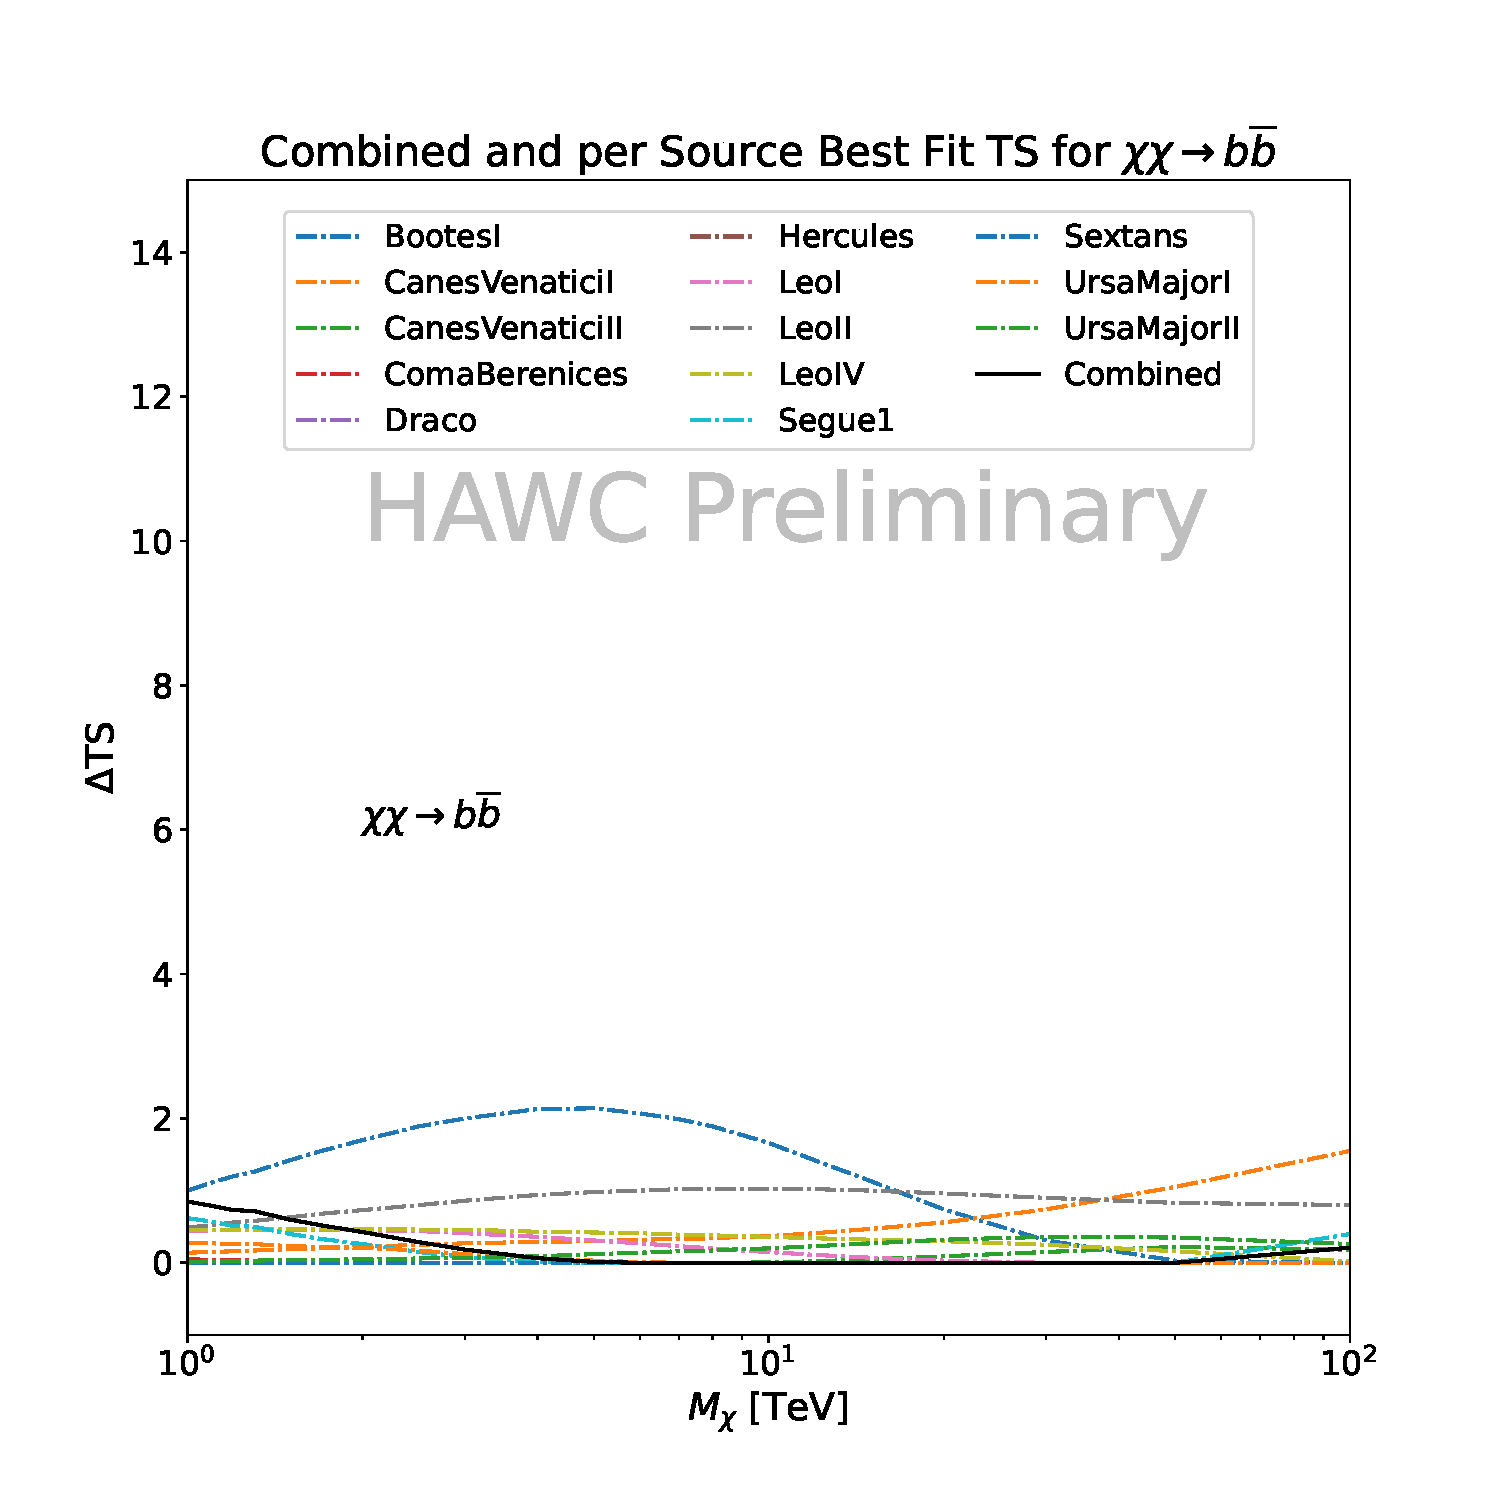
\includegraphics[scale=0.21]{figures/glory_duck/hawc/CombinedTS_data_bb_.pdf}
        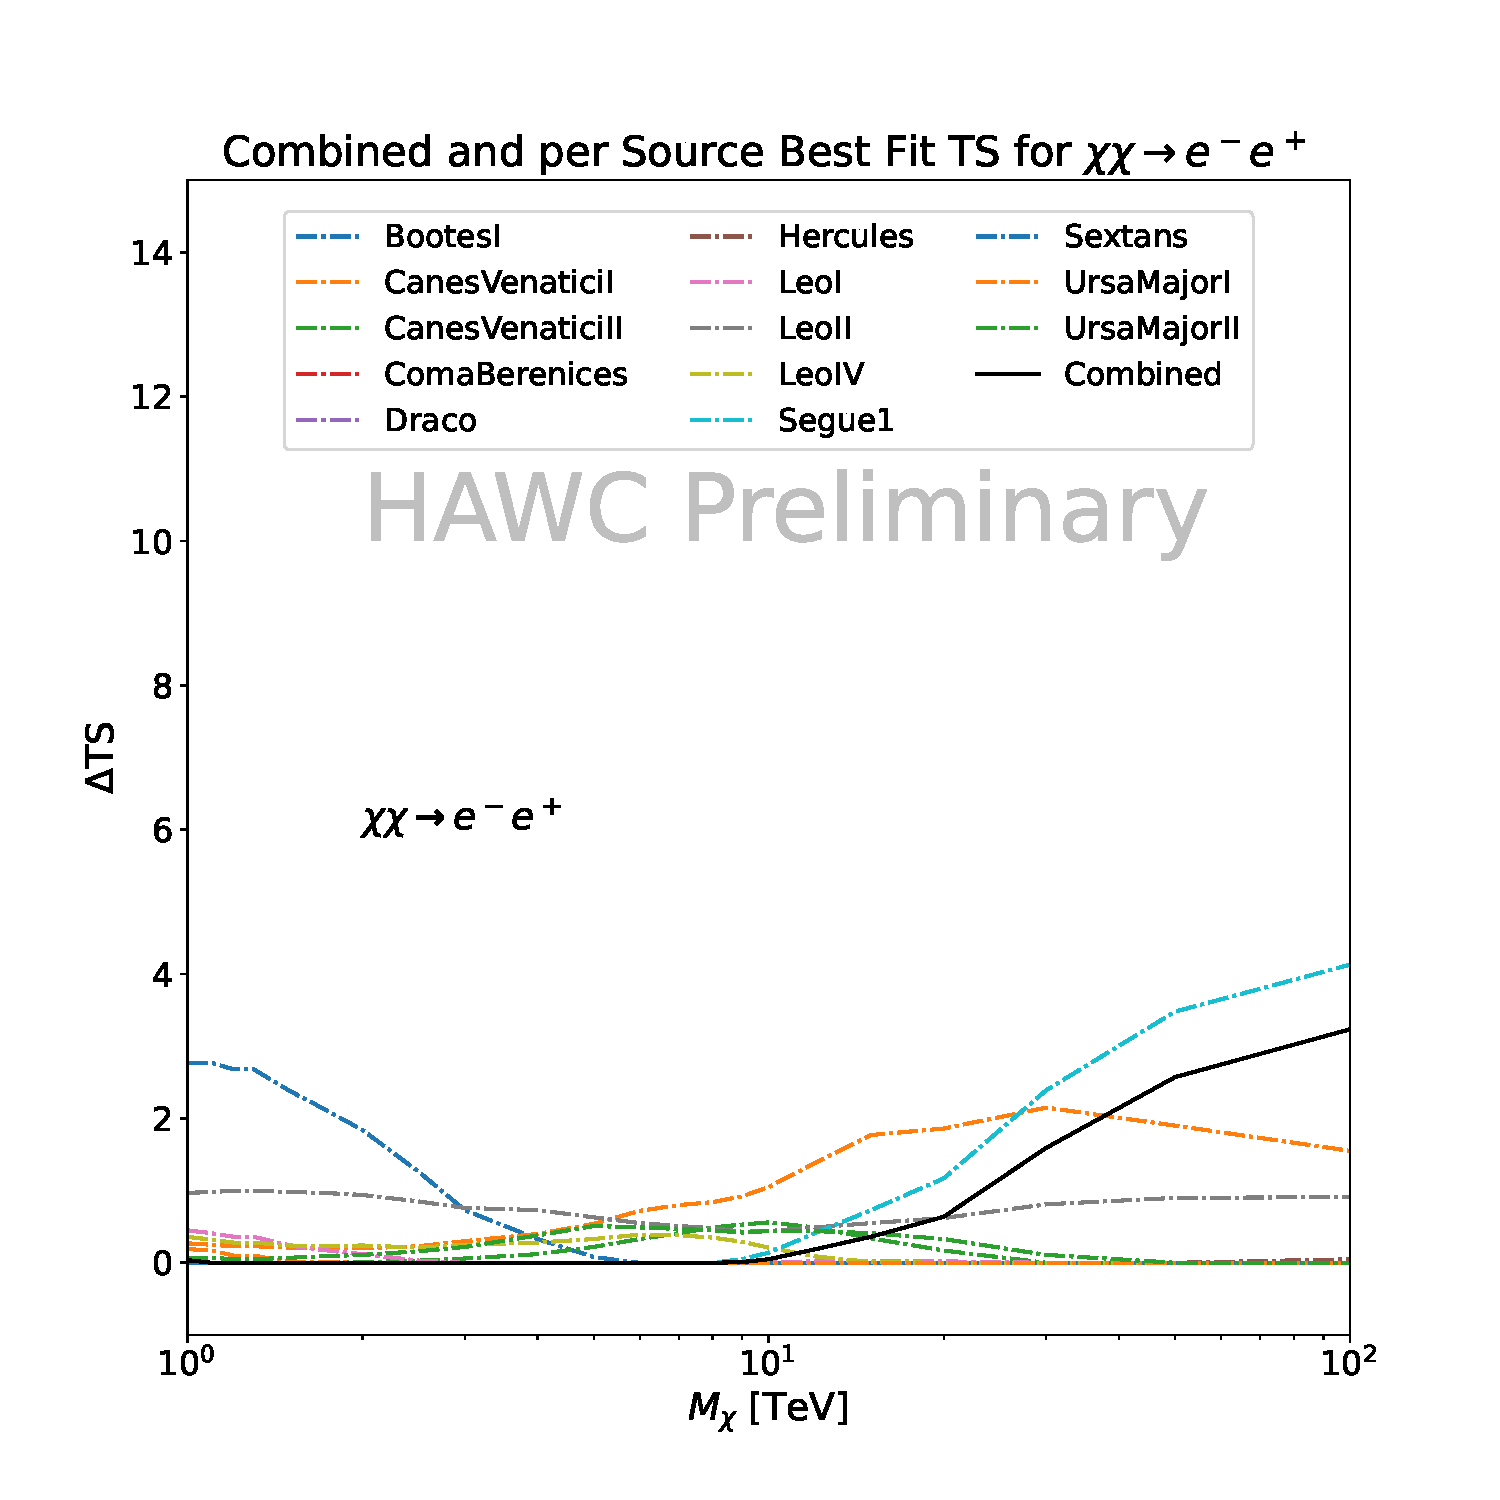
\includegraphics[scale=0.21]{figures/glory_duck/hawc/CombinedTS_data_ee_.pdf}
        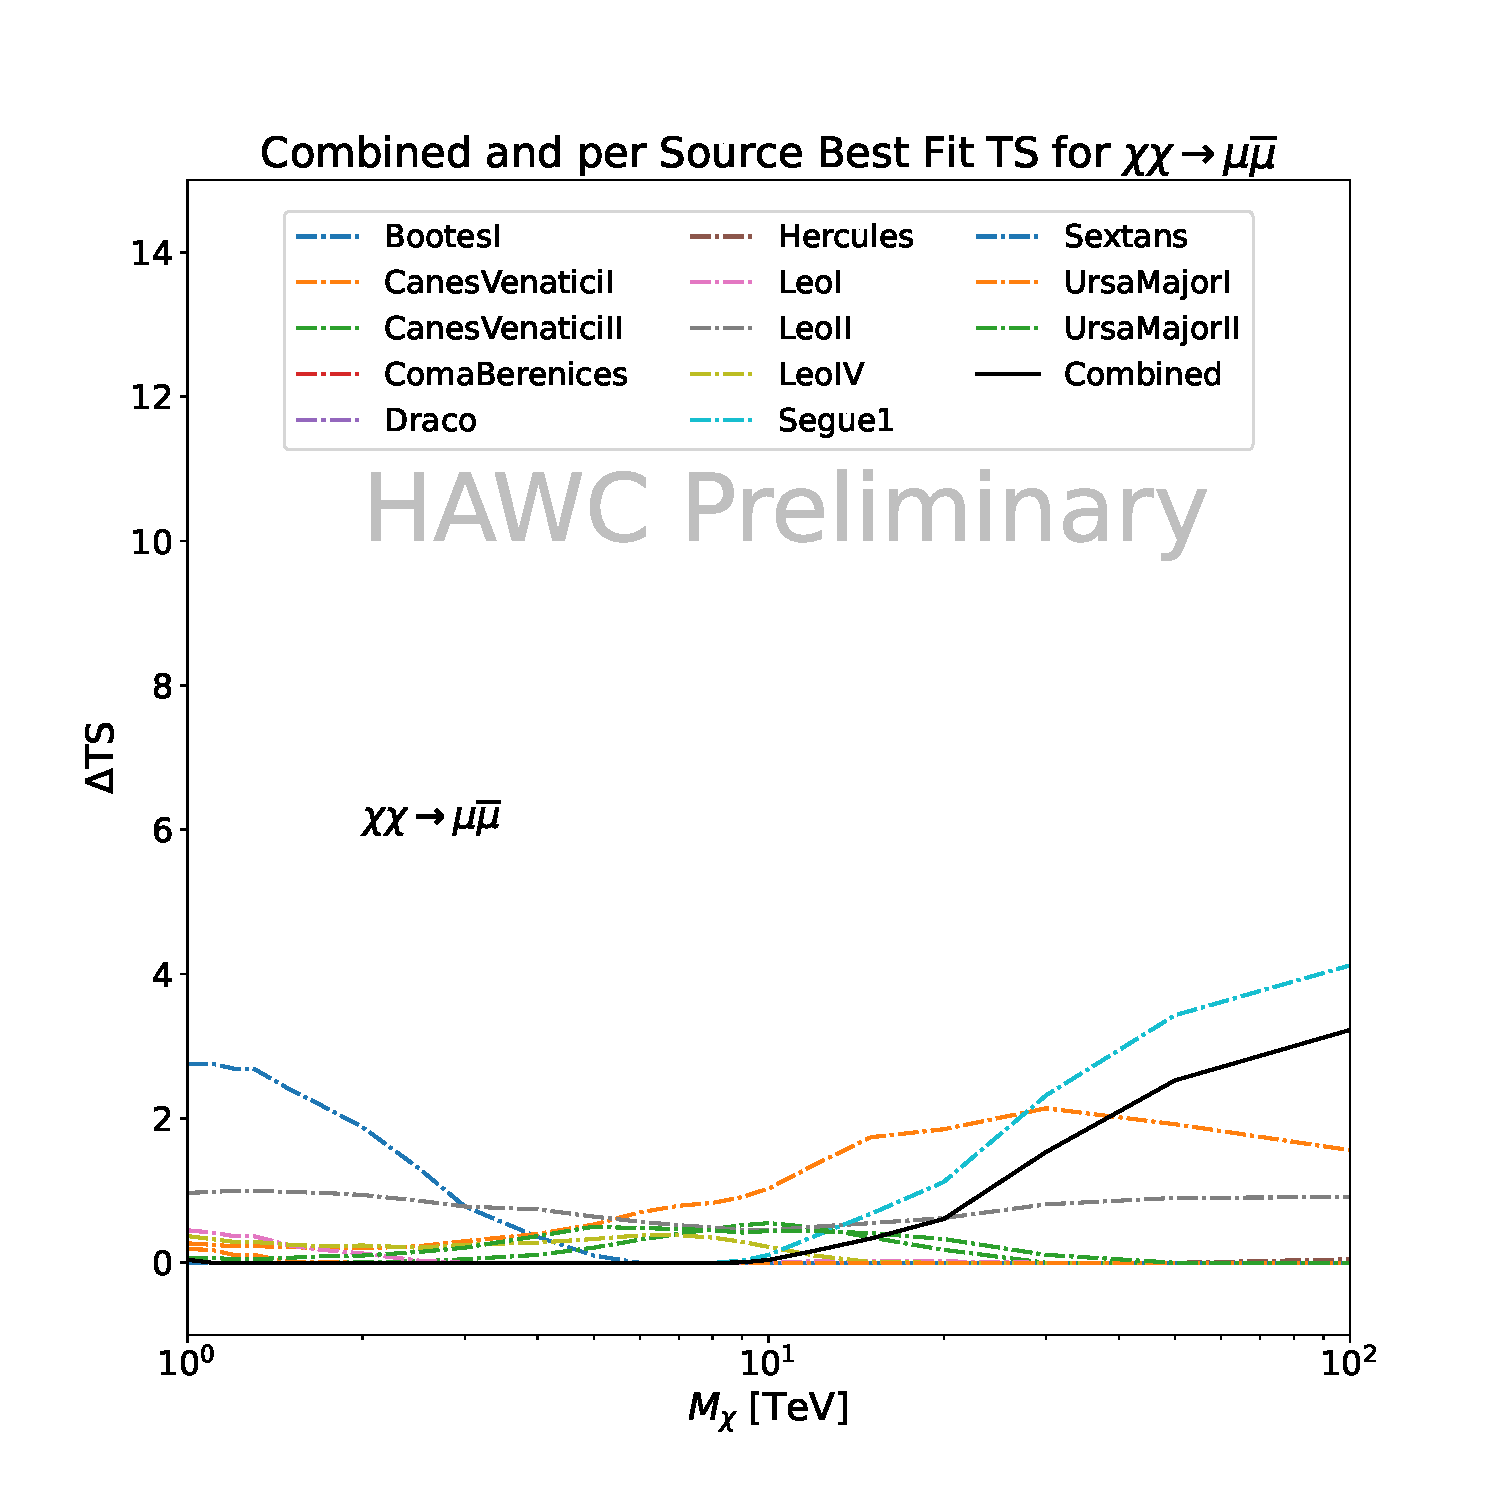
\includegraphics[scale=0.21]{figures/glory_duck/hawc/CombinedTS_data_mumu_.pdf}
        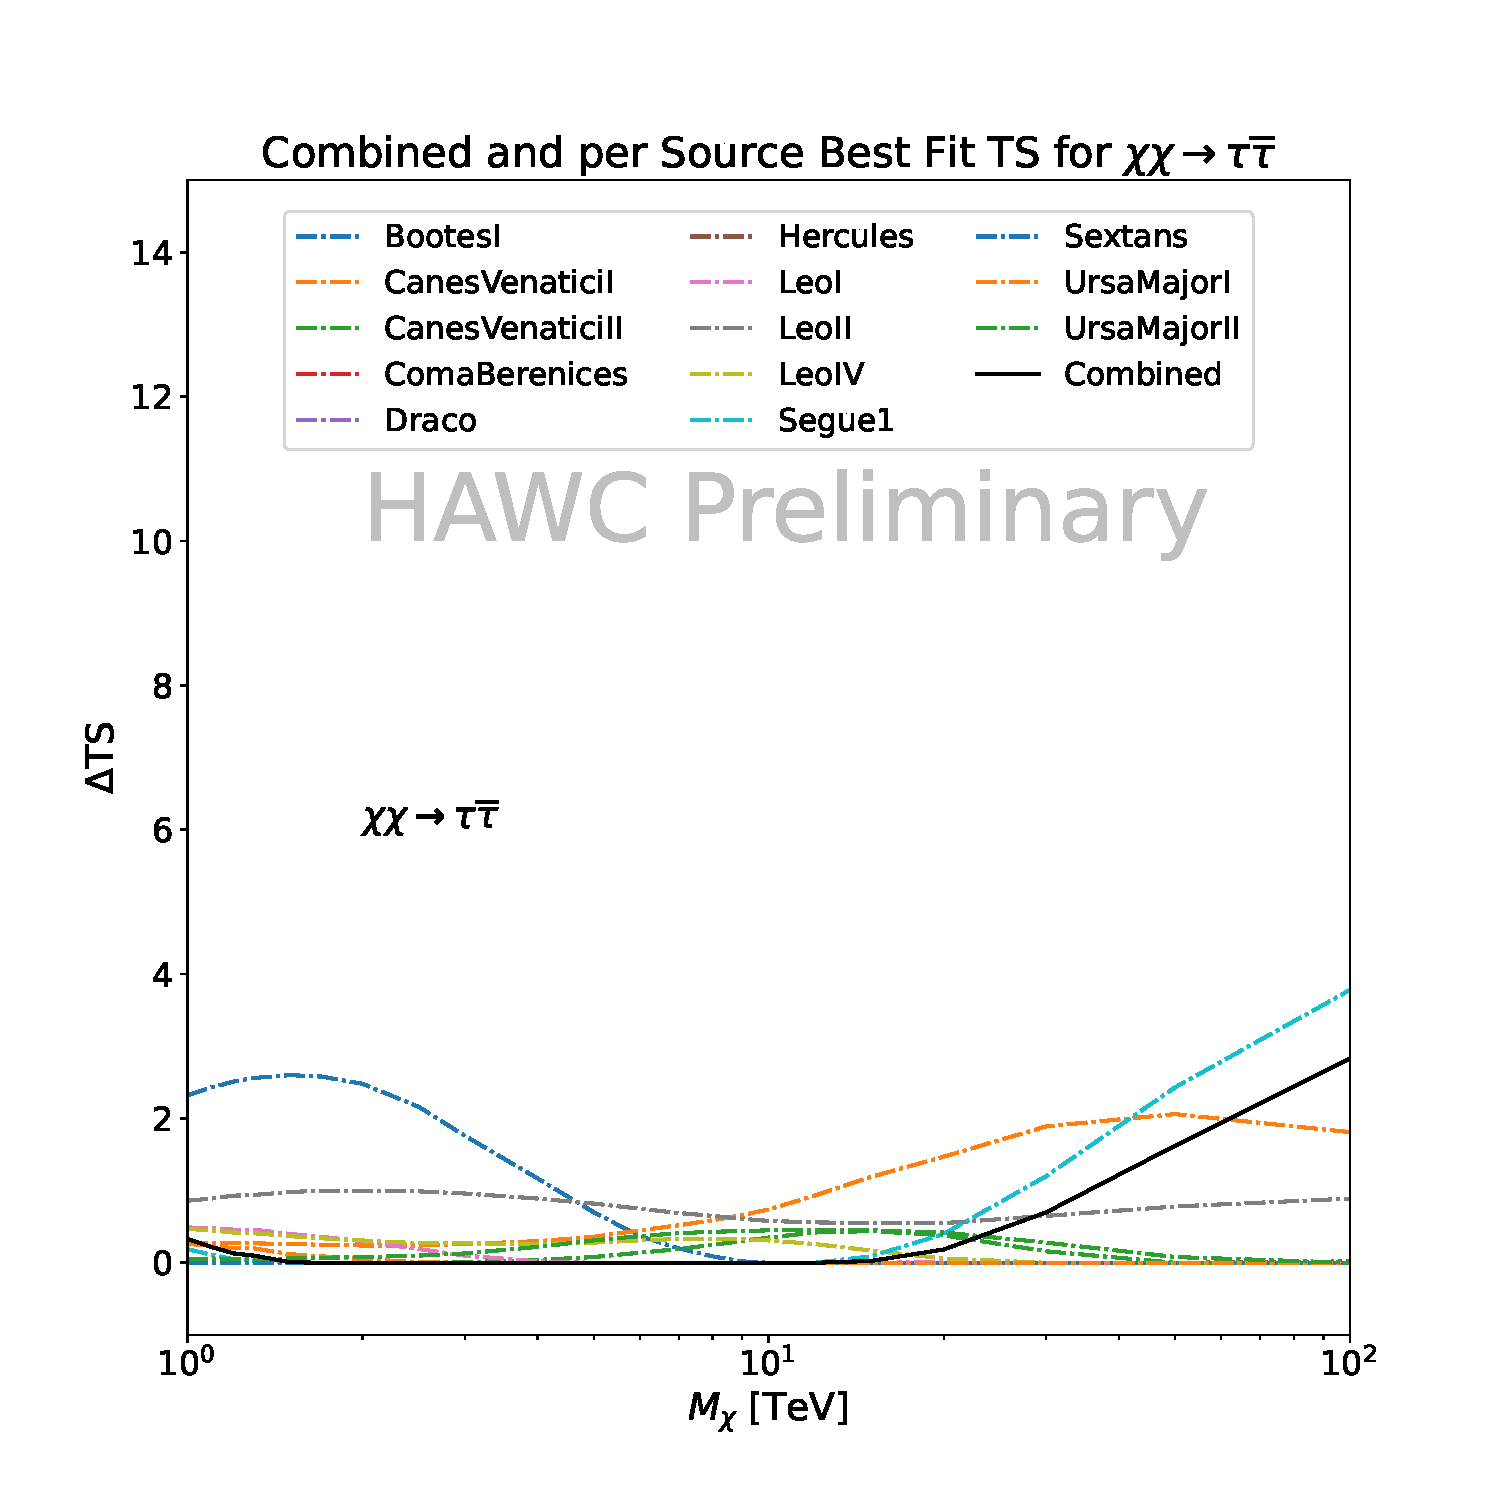
\includegraphics[scale=0.21]{figures/glory_duck/hawc/CombinedTS_data_tautau_.pdf}
        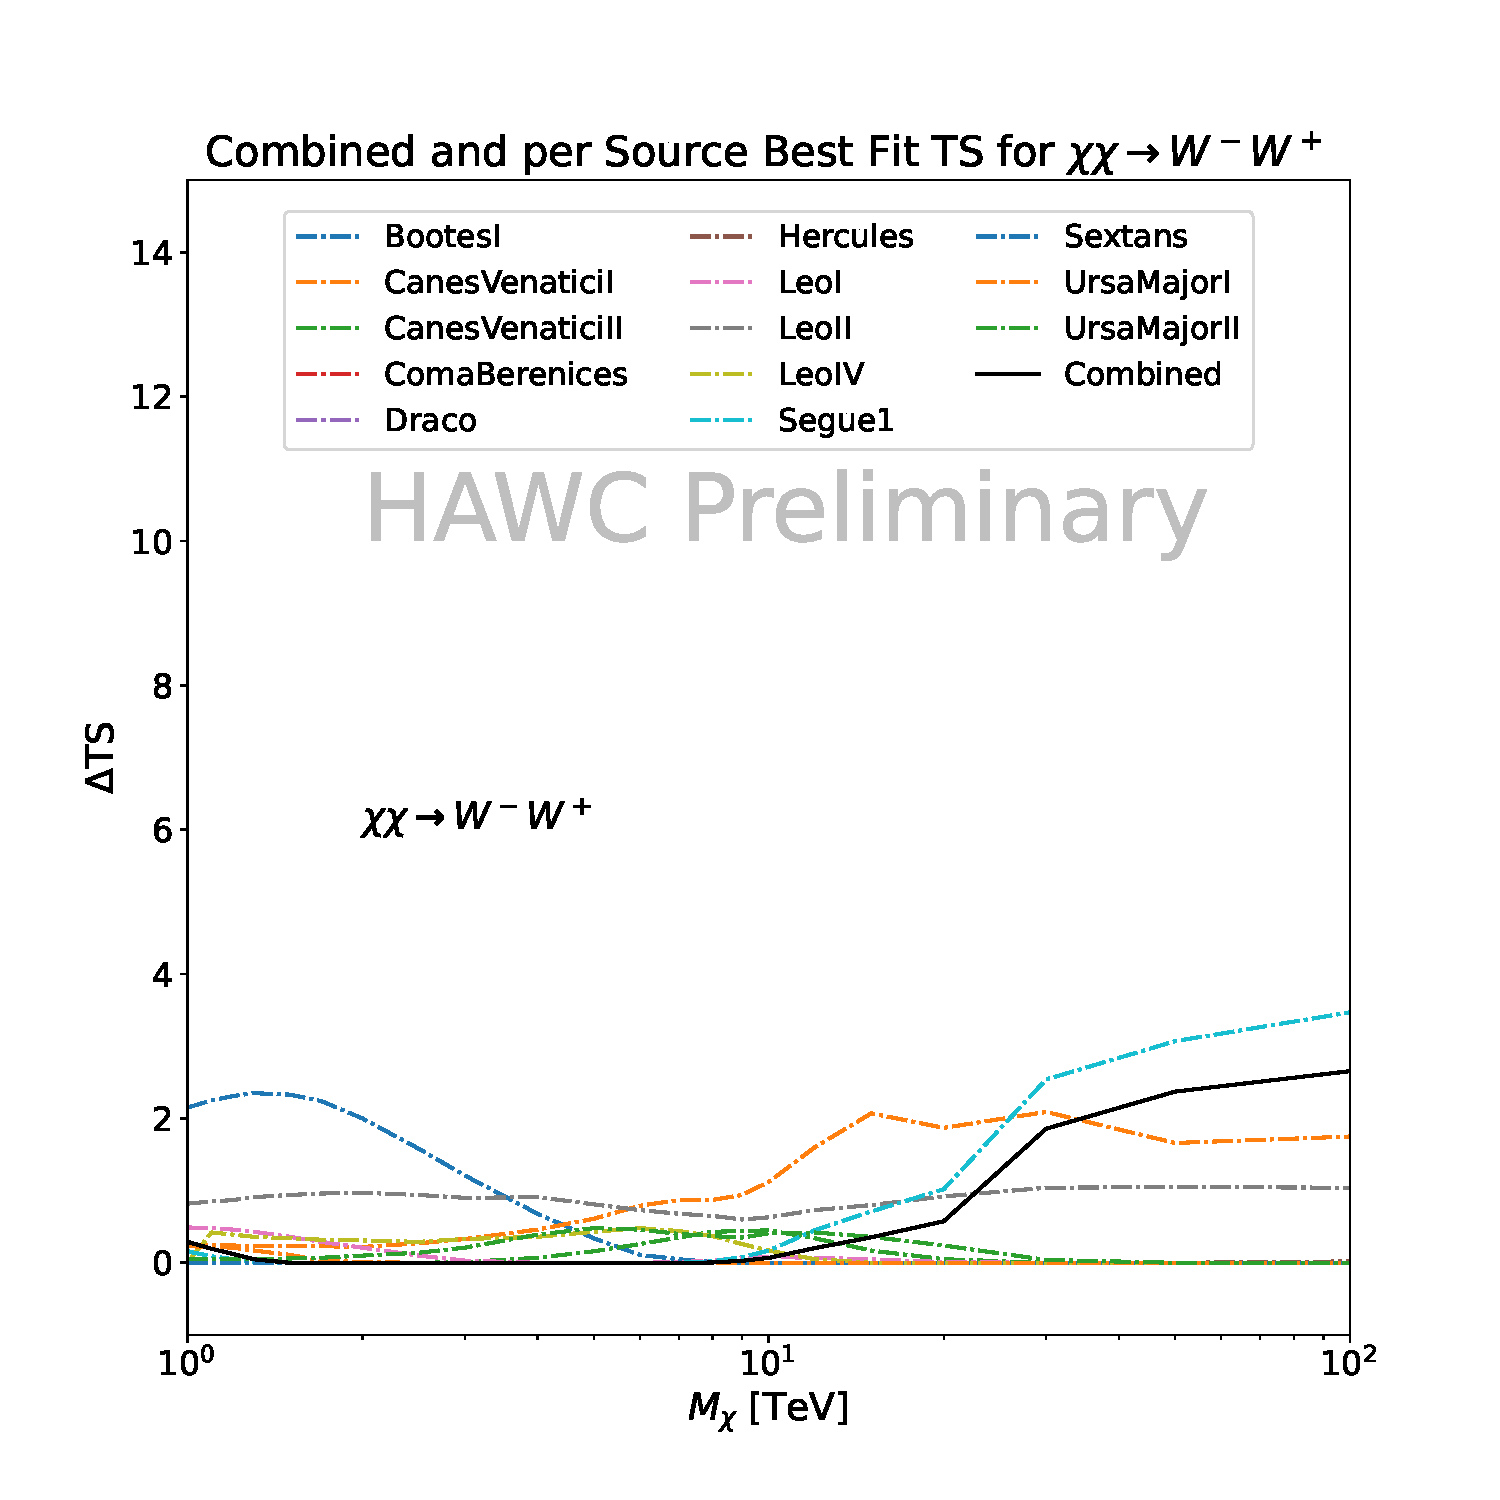
\includegraphics[scale=0.21]{figures/glory_duck/hawc/CombinedTS_data_ww_.pdf}
        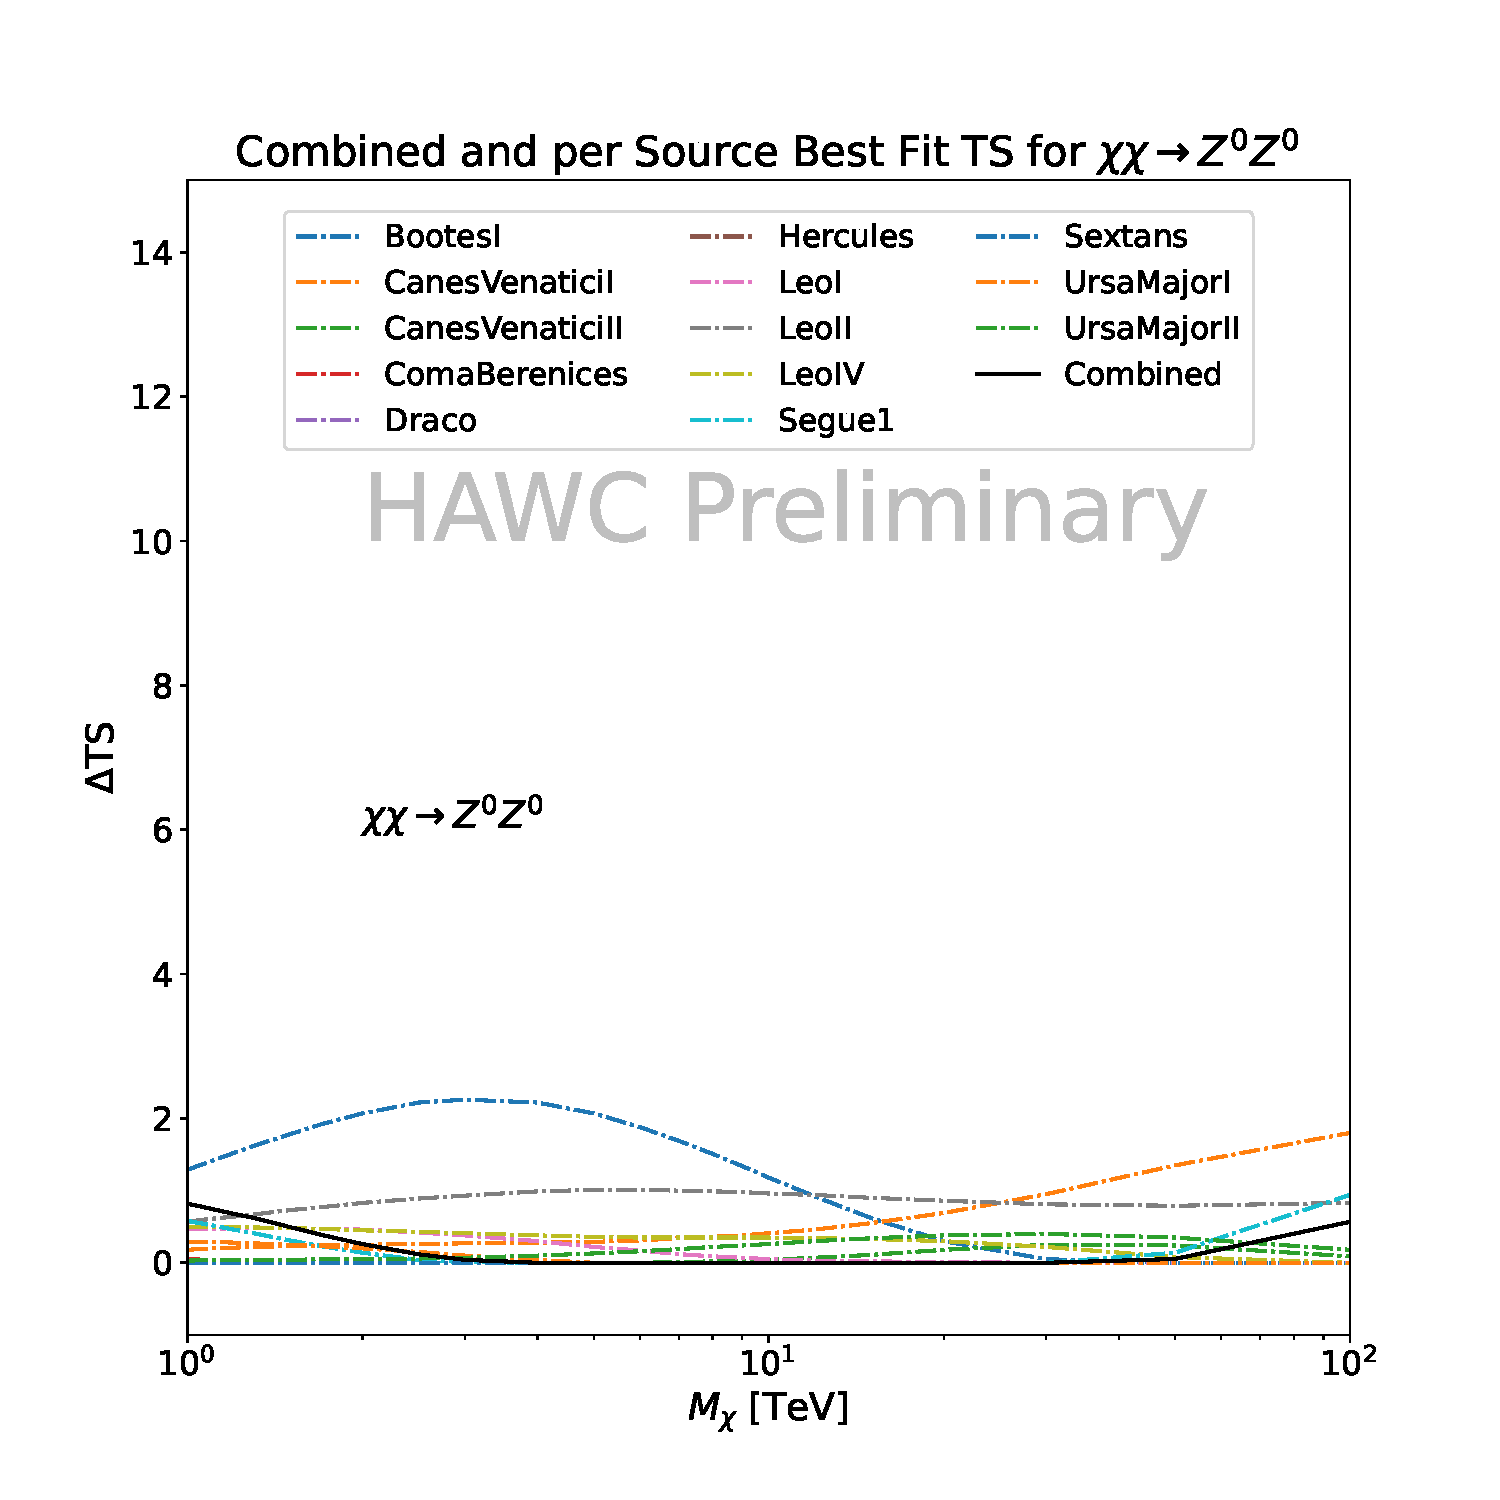
\includegraphics[scale=0.21]{figures/glory_duck/hawc/CombinedTS_data_zz_.pdf}
        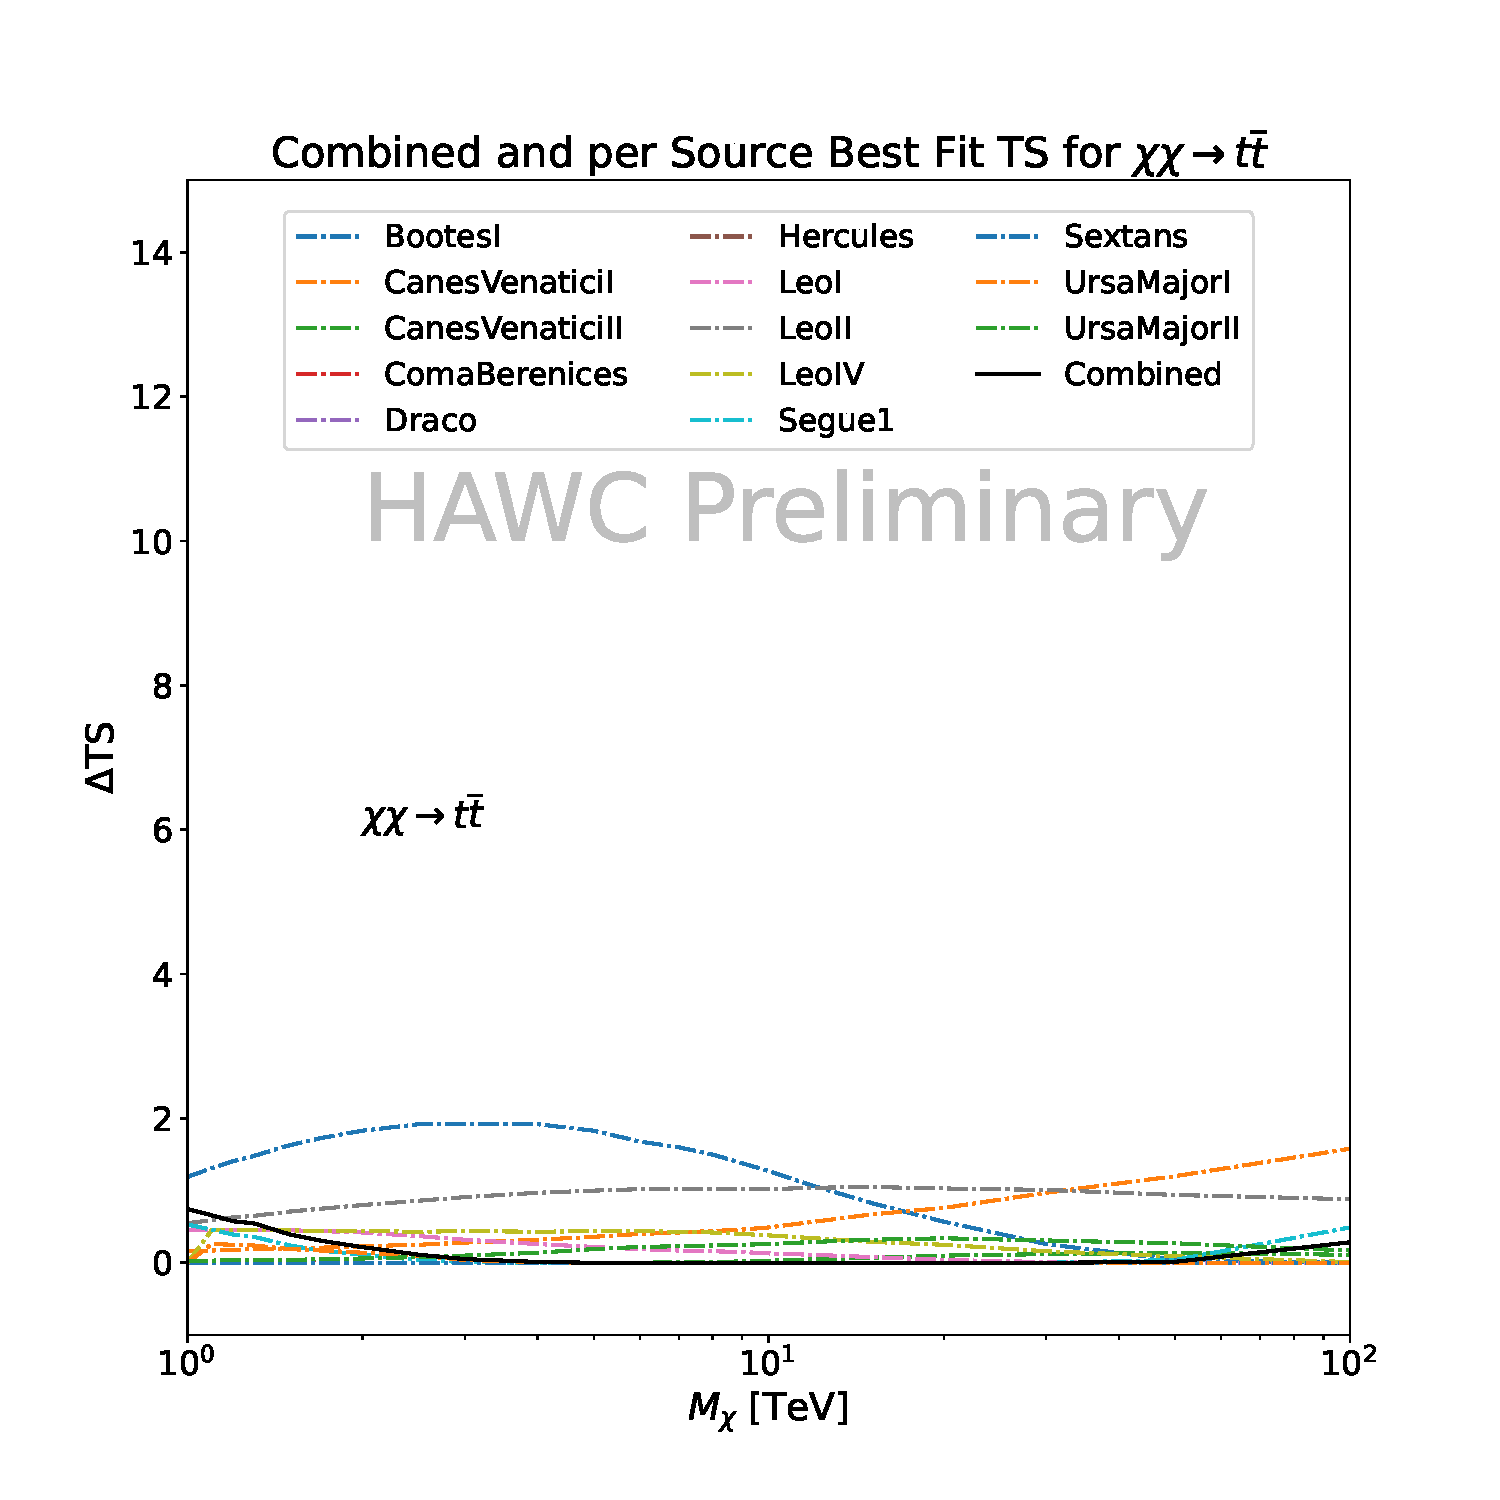
\includegraphics[scale=0.21]{figures/glory_duck/hawc/CombinedTS_data_tt_.pdf}
    }
    \caption{HAWC TS values for best fit \sv~versus $m_\chi$ for seven SM annihilation channels with \J factors from \GS. The solid black line shows the combined best fit TS values. The colored, dashed lines are the TS values for each of the 13 sources HAWC studied.}\label{fig:gd_HAWC_TS}
\end{figure}

No DM was found in HAWC observations.
HAWC's limits are dominated by the dSphs Segue1 and Coma Berenices.
The remaining 11 dSphs do not contribute significantly to the limit because they are at high zenith and/or have much smaller \J factors.
Even though some remaining dSphs have large \J factors, they are towards the edge of HAWC's field of view where HAWC analysis is less sensitive.

\begin{figure}[t]
    \centering{
    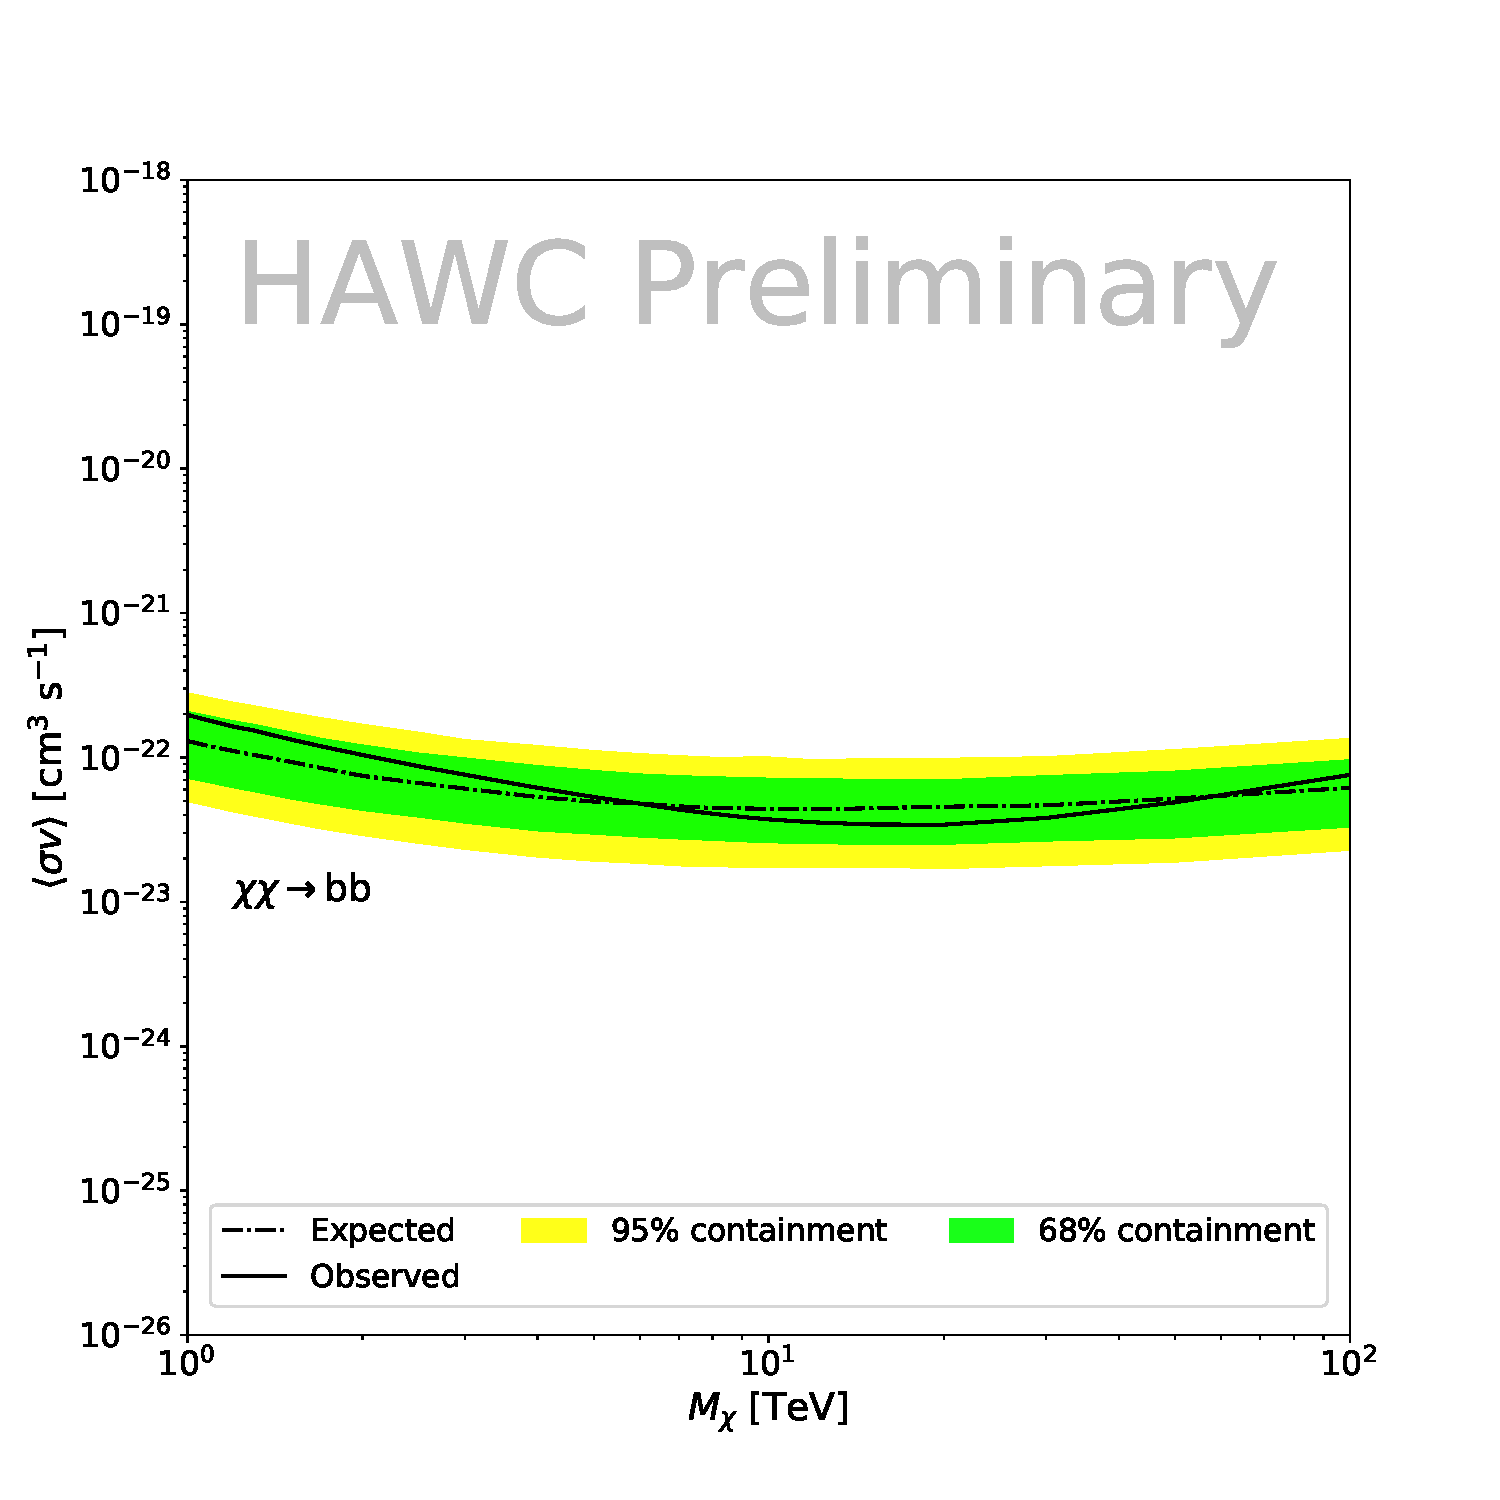
\includegraphics[scale=0.21]{figures/glory_duck/hawc/GD_BrazilBand_bb.pdf}
    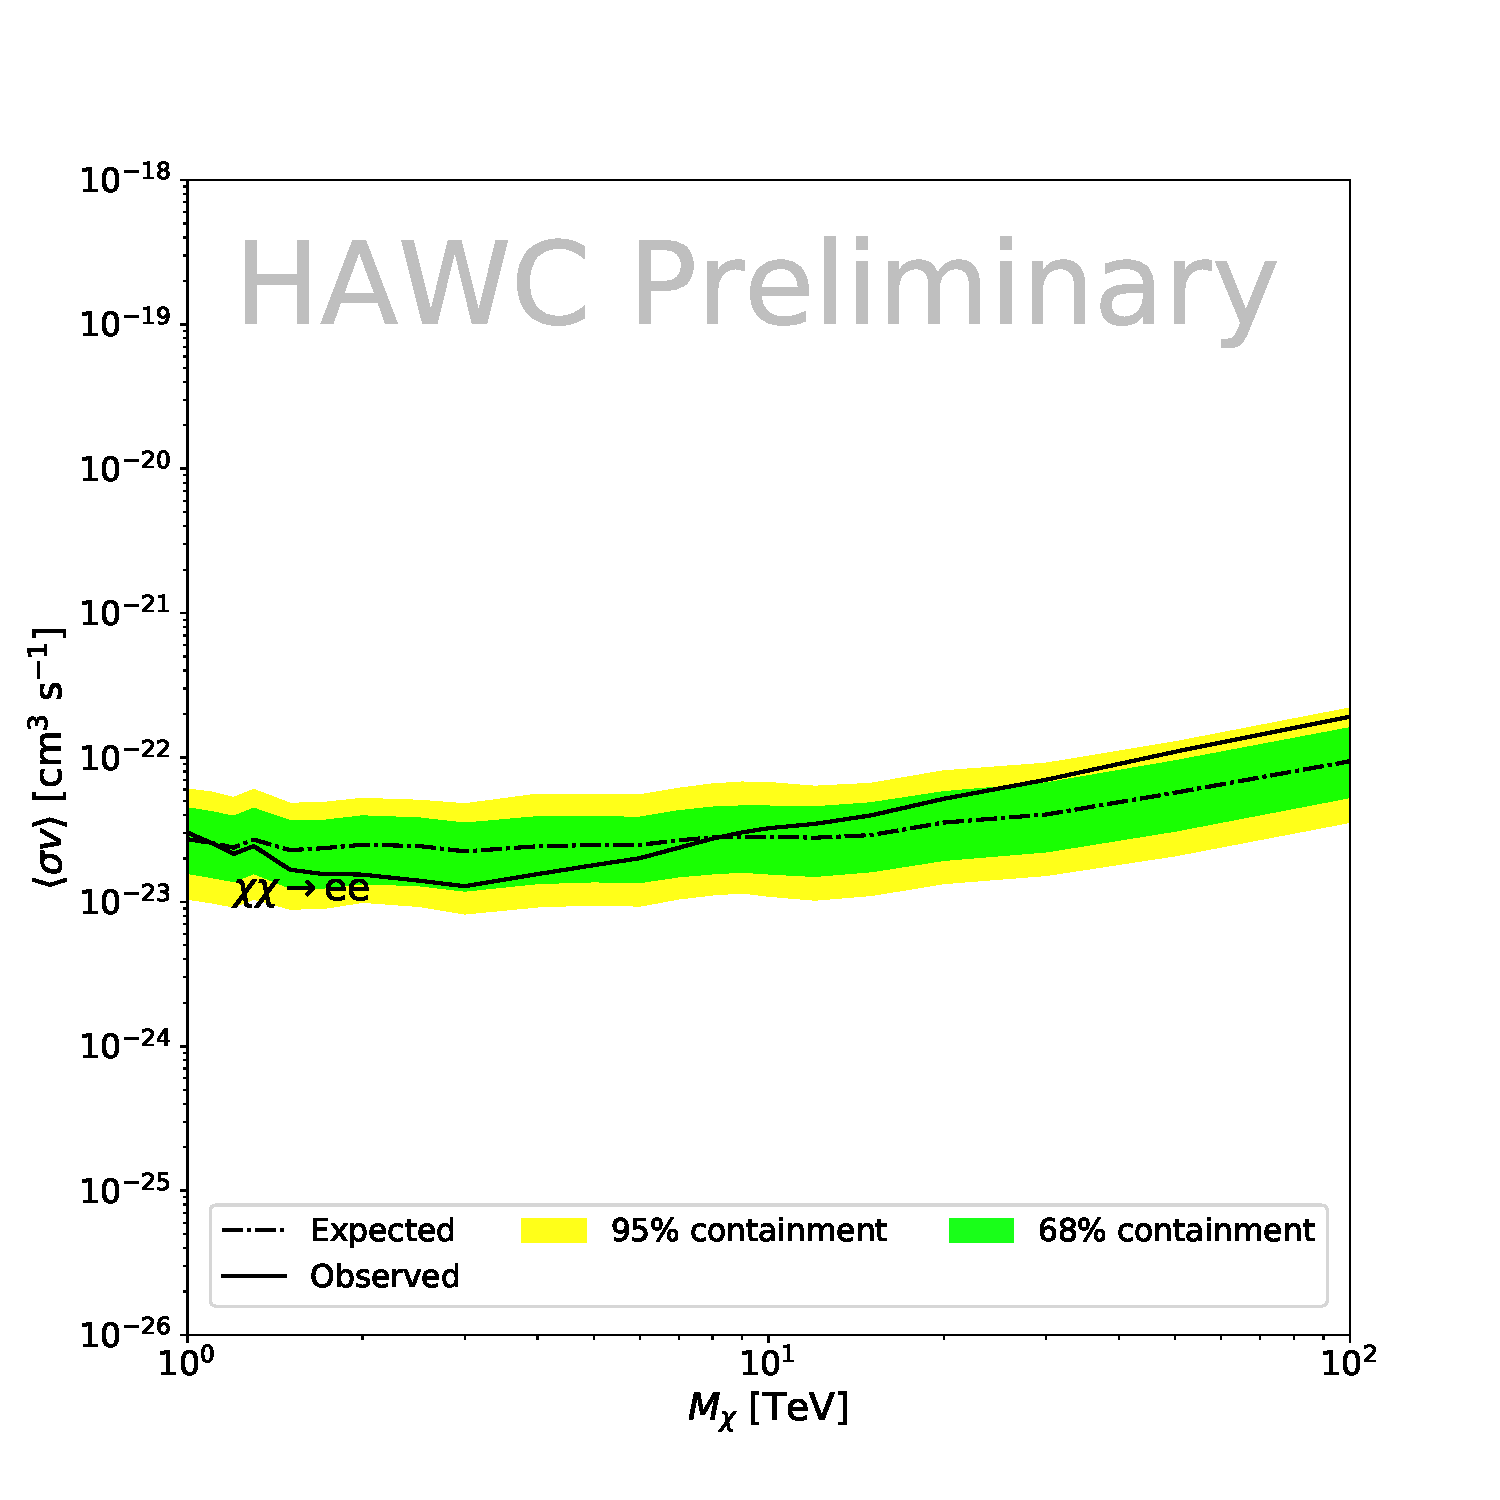
\includegraphics[scale=0.21]{figures/glory_duck/hawc/GD_BrazilBand_ee.pdf}
    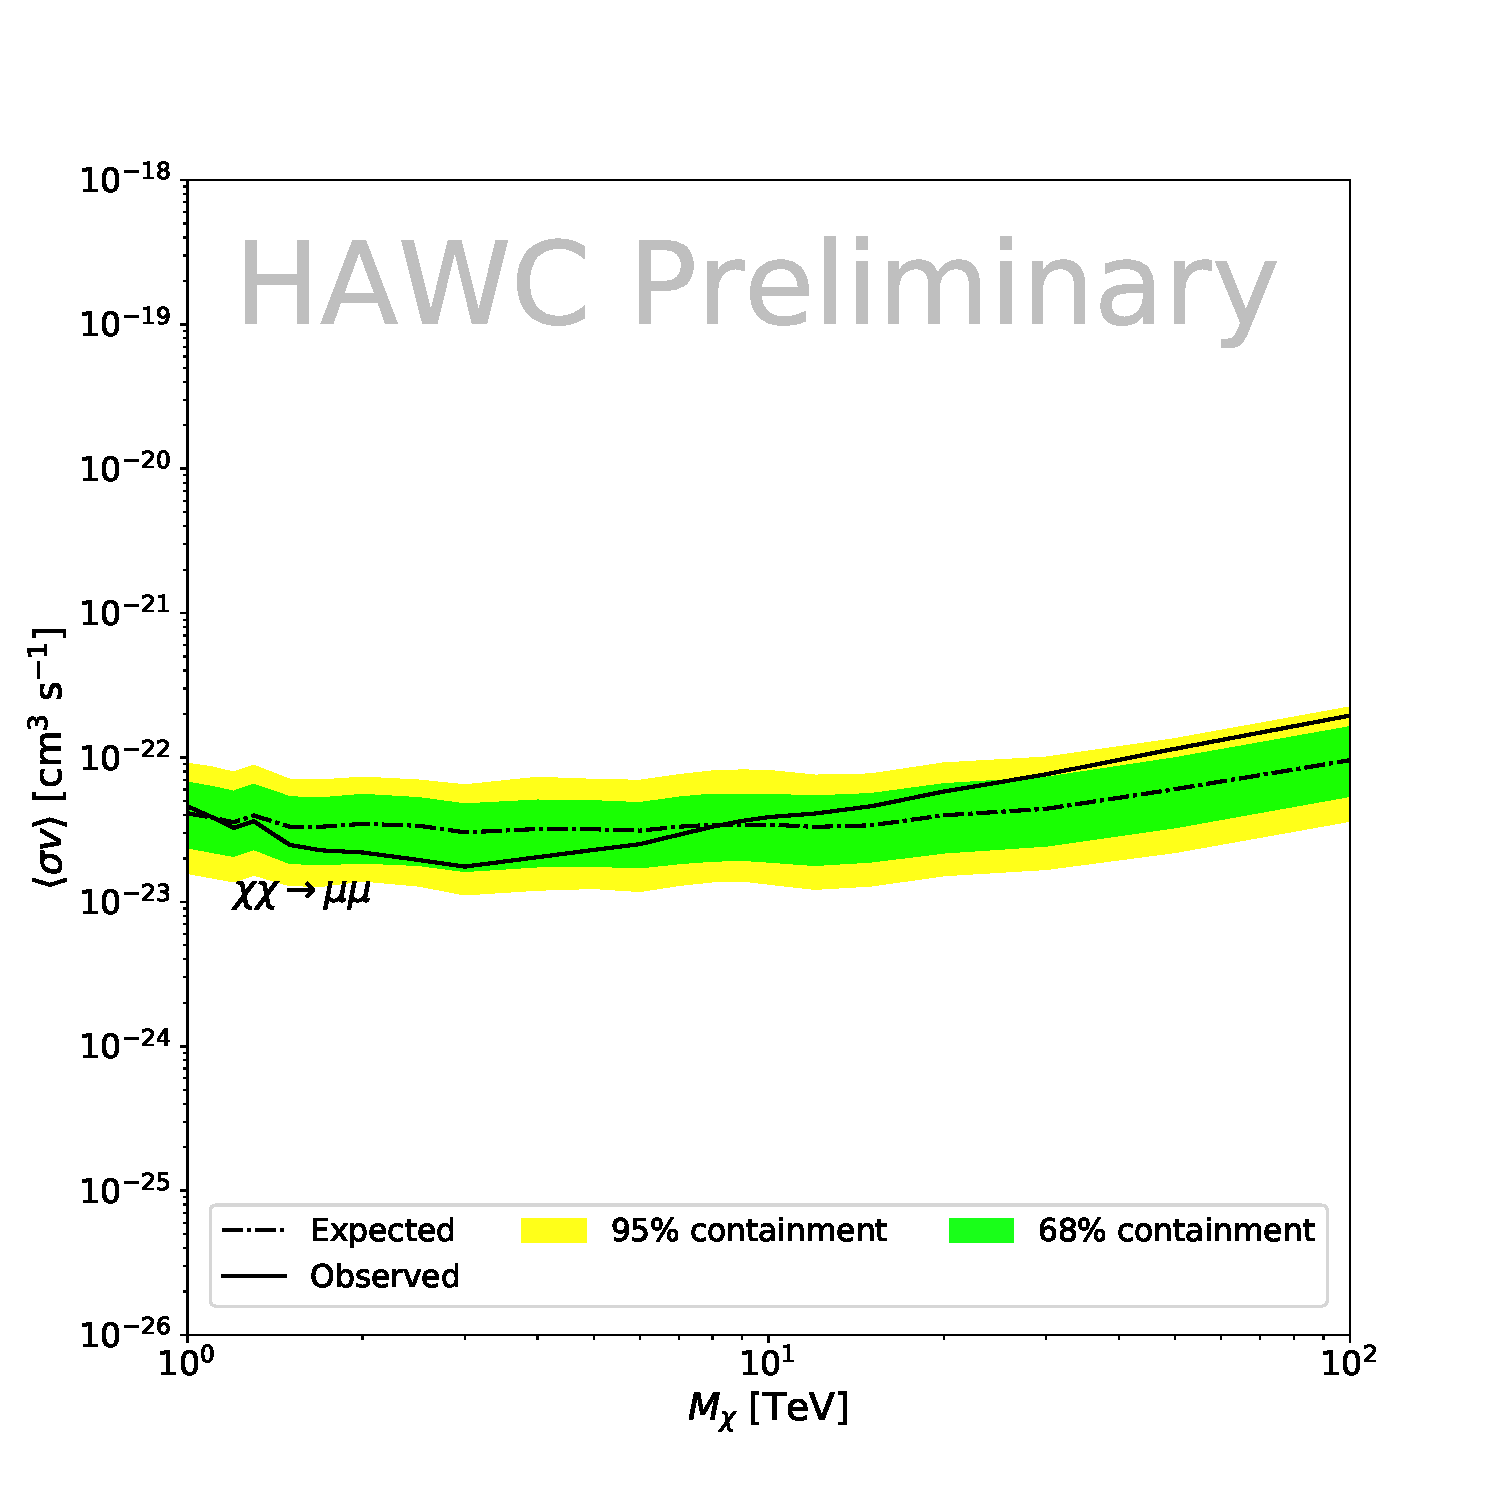
\includegraphics[scale=0.21]{figures/glory_duck/hawc/GD_BrazilBand_mumu.pdf}
    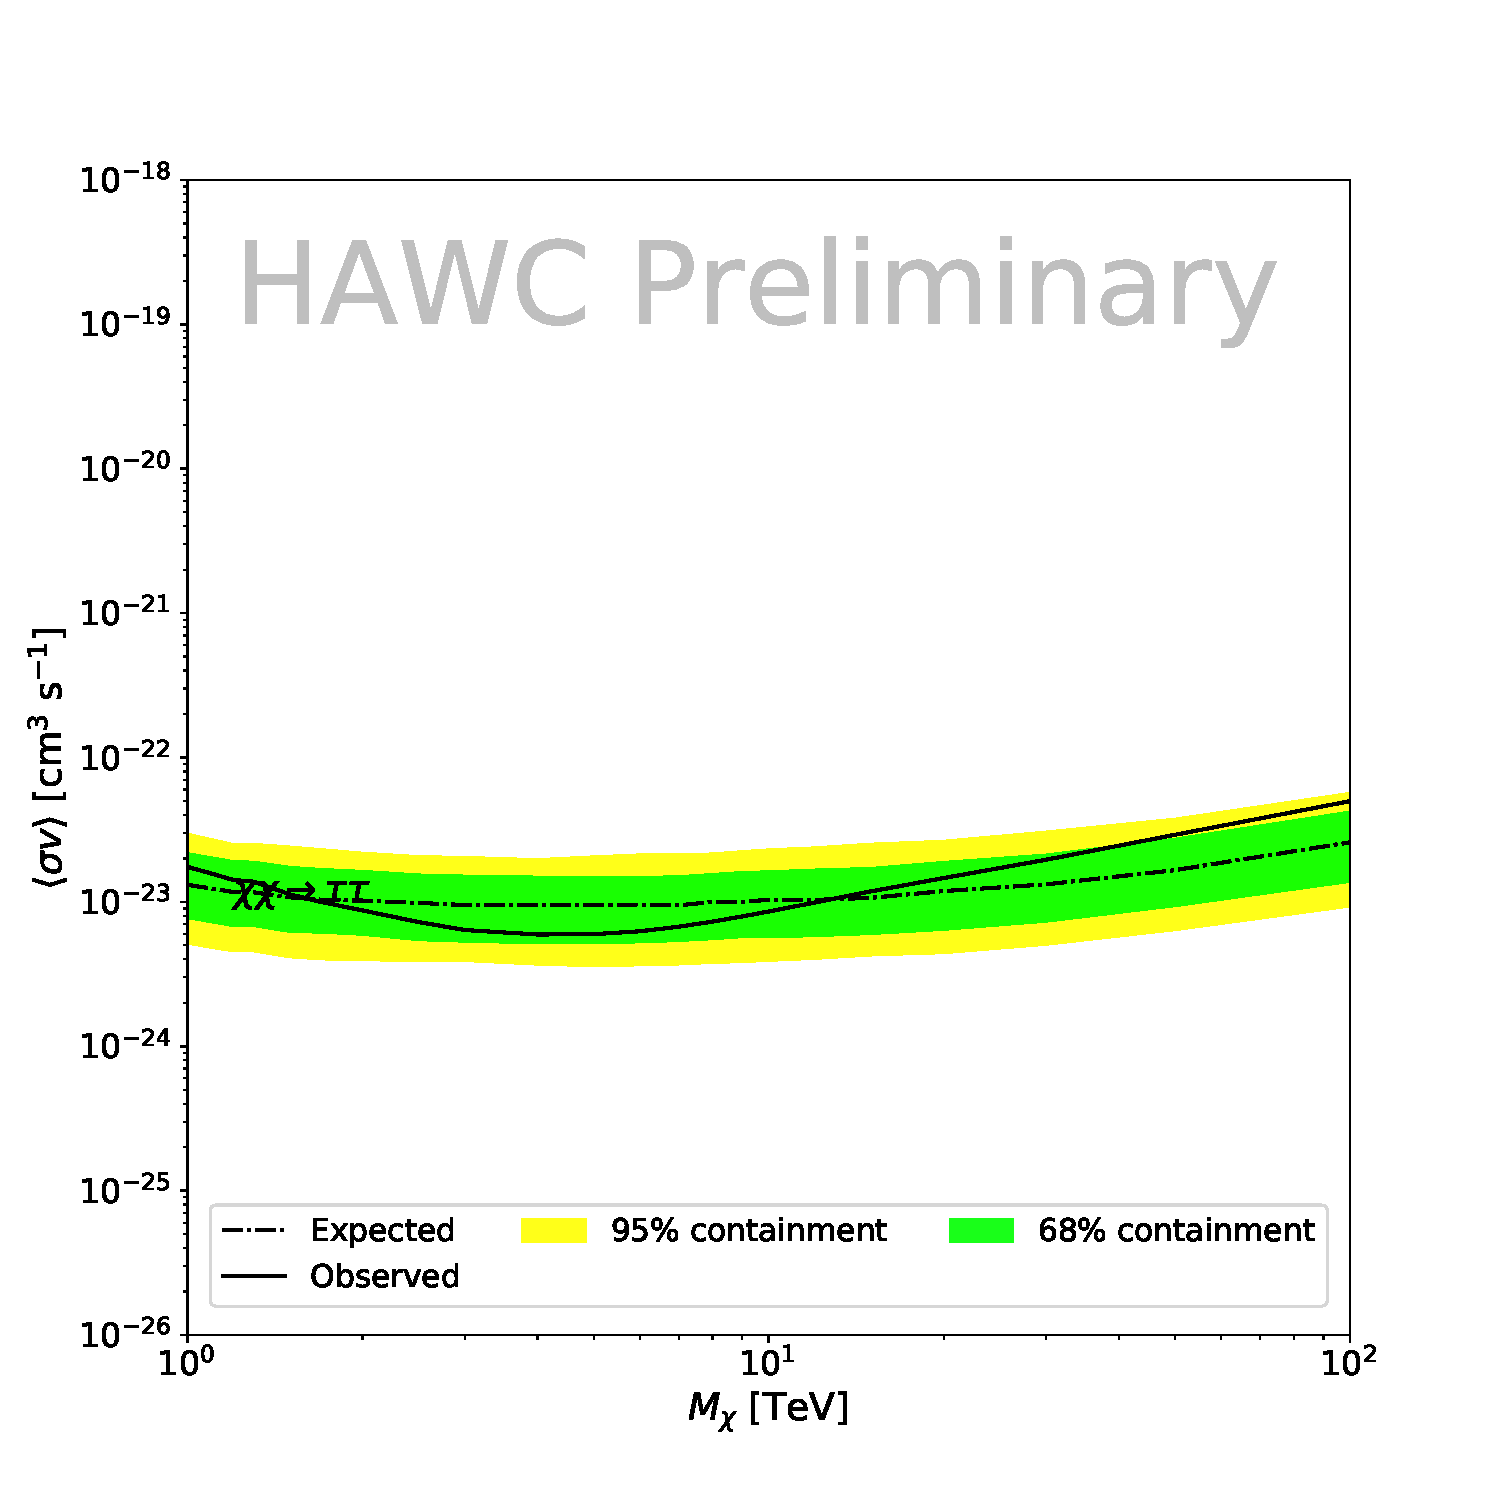
\includegraphics[scale=0.21]{figures/glory_duck/hawc/GD_BrazilBand_tautau.pdf}
    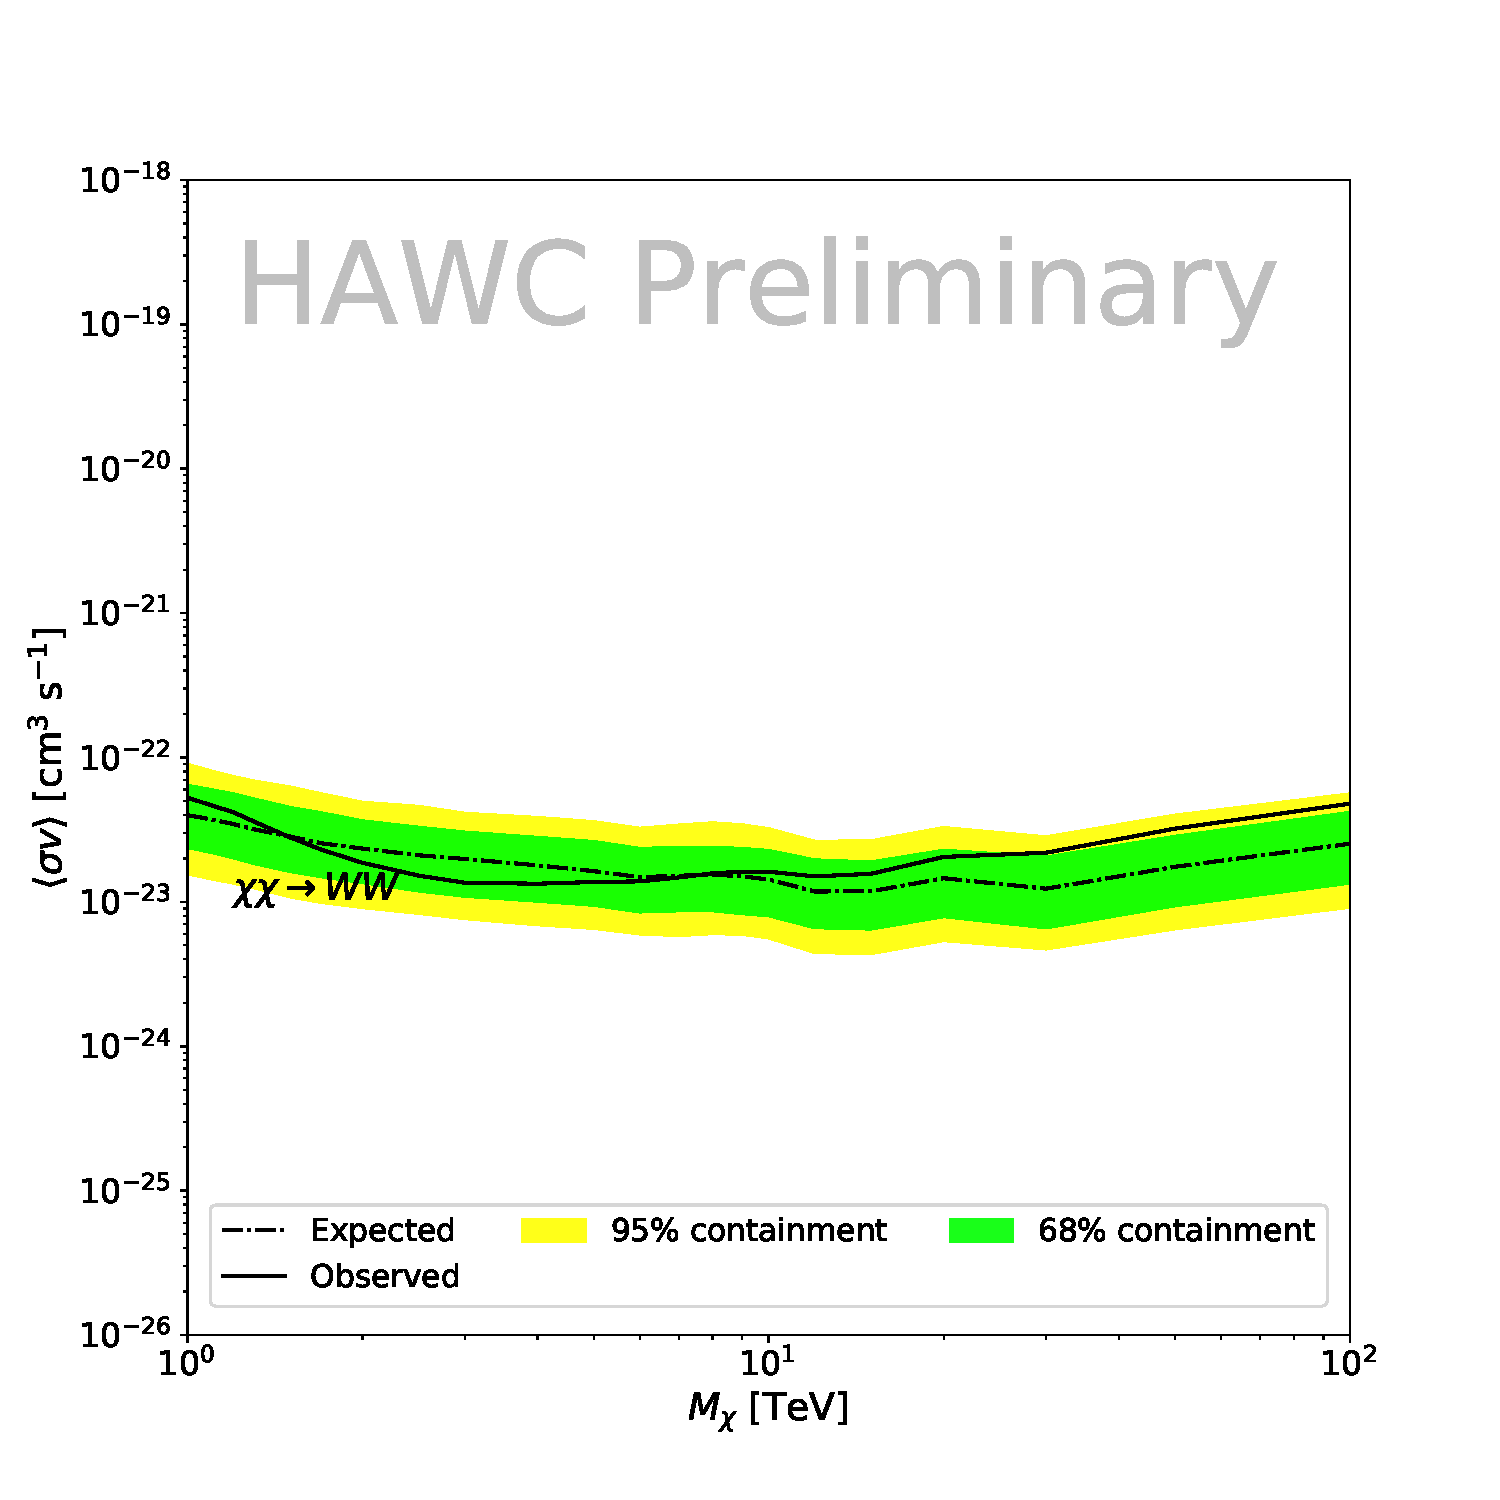
\includegraphics[scale=0.21]{figures/glory_duck/hawc/GD_BrazilBand_ww.pdf}
    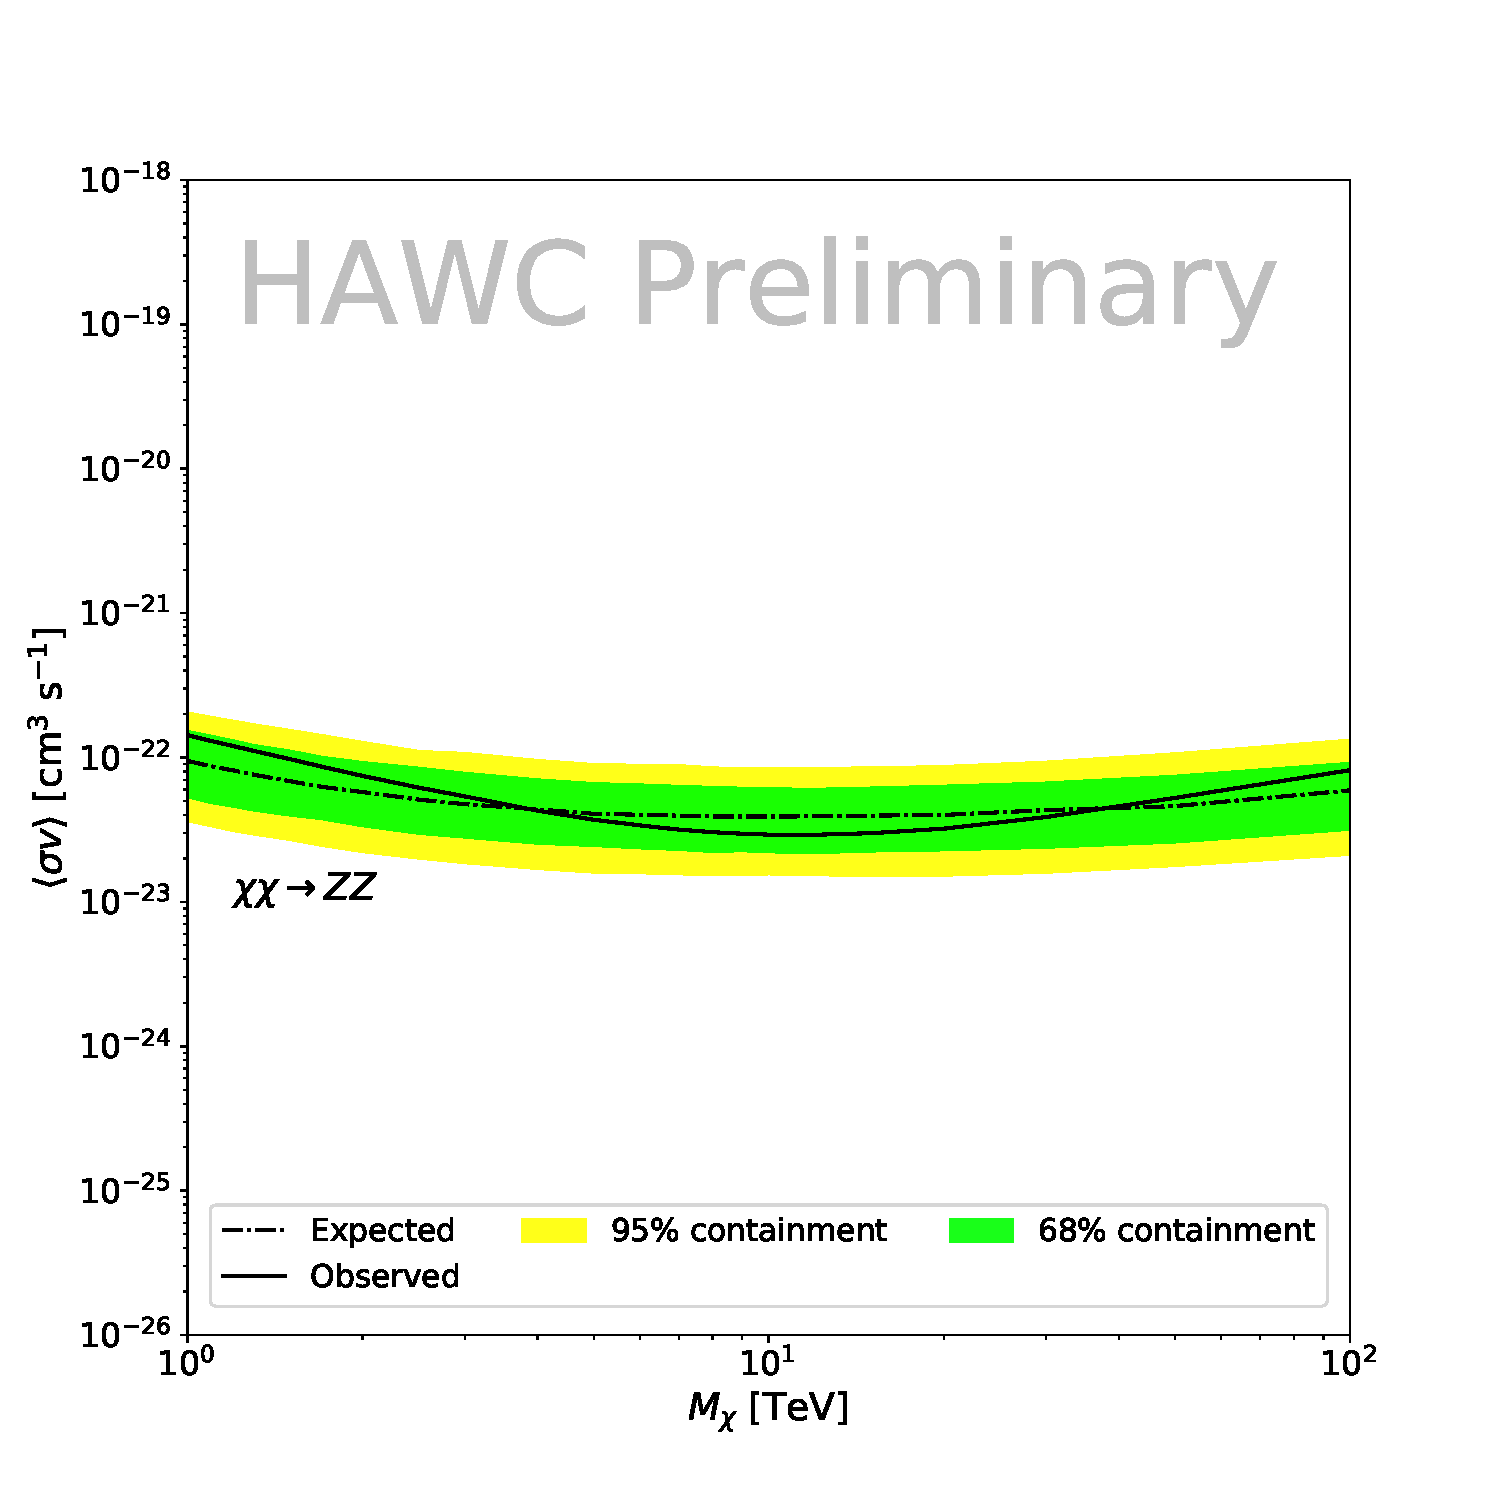
\includegraphics[scale=0.21]{figures/glory_duck/hawc/GD_BrazilBand_zz.pdf}
    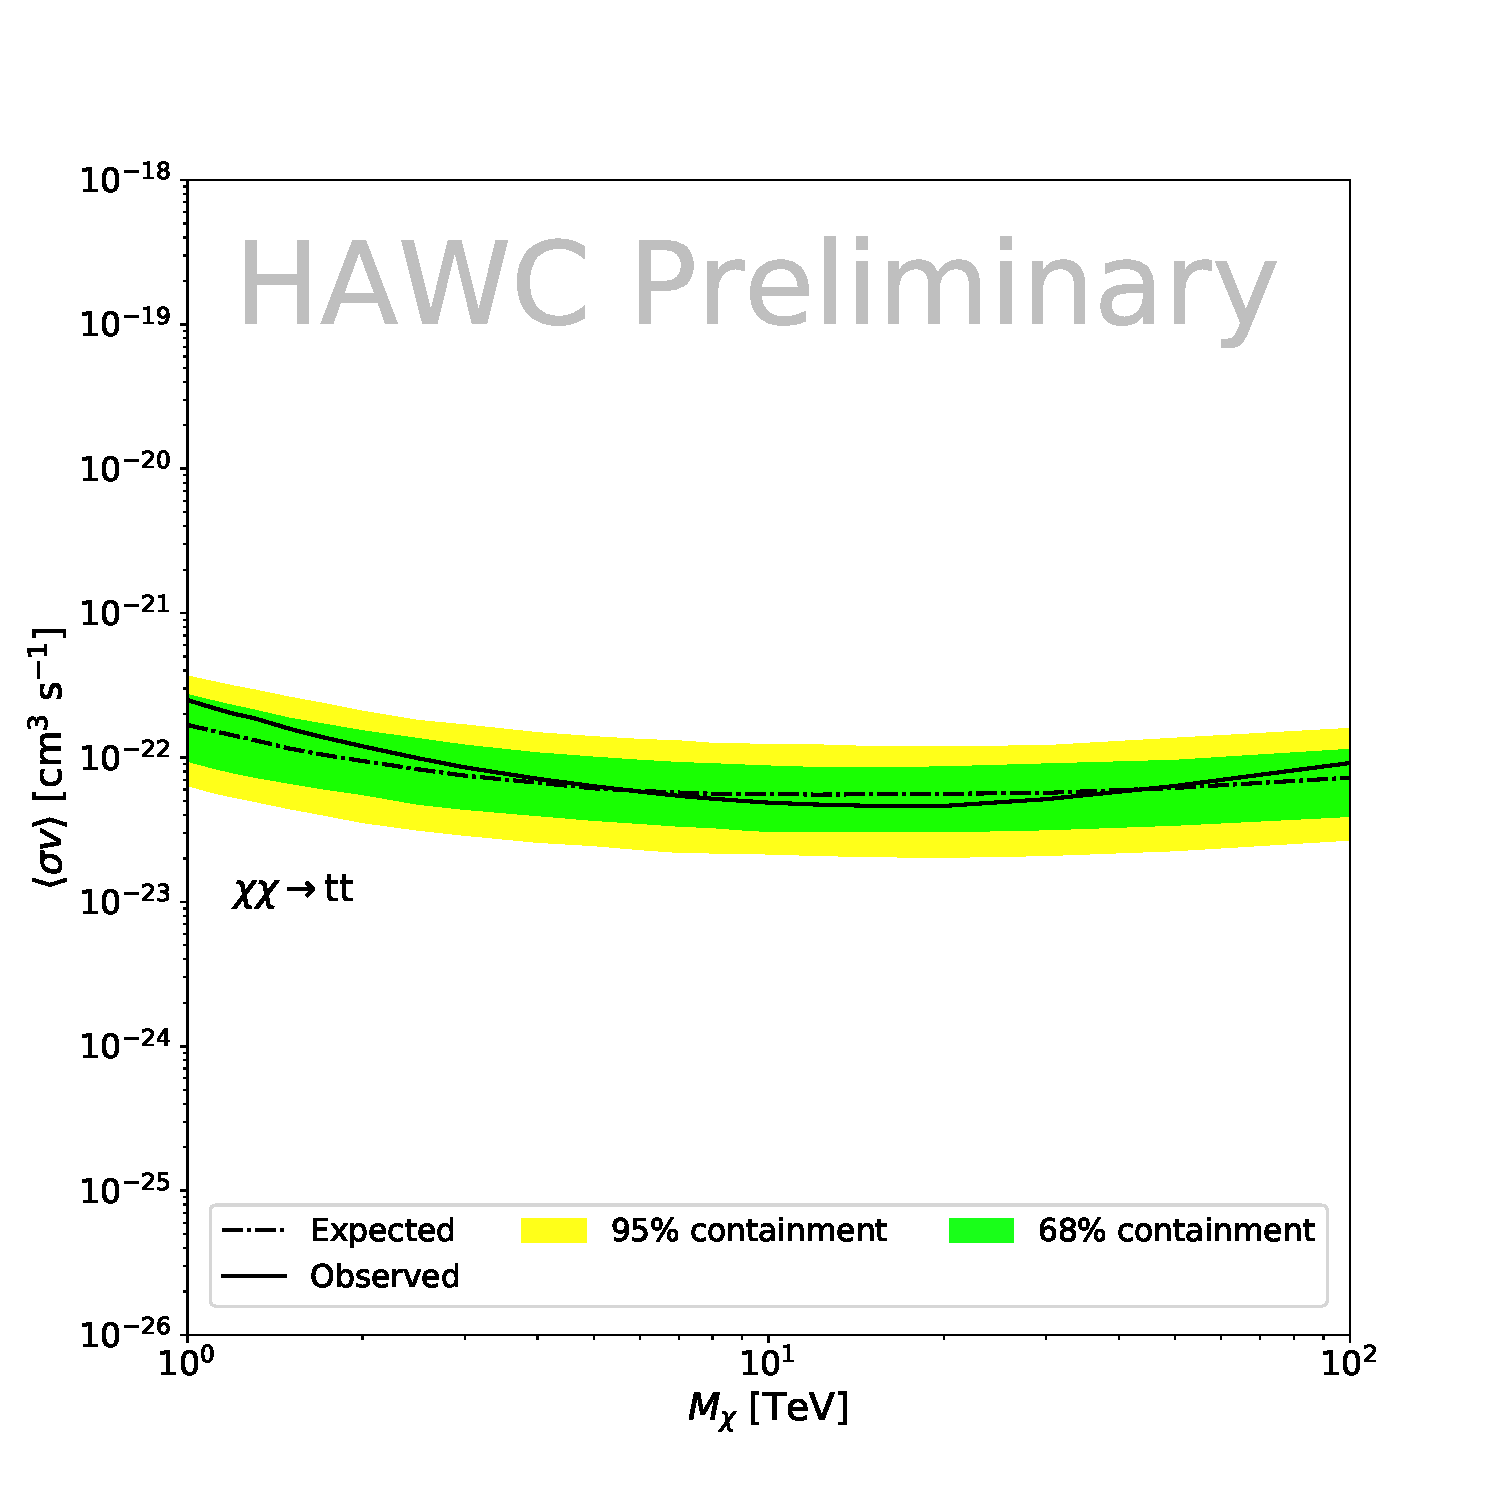
\includegraphics[scale=0.21]{figures/glory_duck/hawc/GD_BrazilBand_tt.pdf}
    }
    \caption{HAWC Brazil bands at 95\% confidence level on \sv versus DM mass for seven annihilation channels with \J-factors from \GS \cite{Geringer-Sameth:2014yza}. The solid line represents the combined limit from 13 dSphs. The dashed line is the expected limit. The green band is the 68\% containment. The yellow band is the 95\% containment.}
\label{fig:hawc_brazil_band}
\end{figure}

%%%%%%%%%%%%%%%%%%%%%%%%%%%%%%%%%%%%%%%%%%%%%%%%%%%%%%%
\section{Glory Duck Combined Results}\label{sec:results}
%%%%%%%%%%%%%%%%%%%%%%%%%%%%%%%%%%%%%%%%%%%%%%%%%%%%%%%

\begin{figure}[ht!]
    \centering{
    \begin{tabular}{cc}
        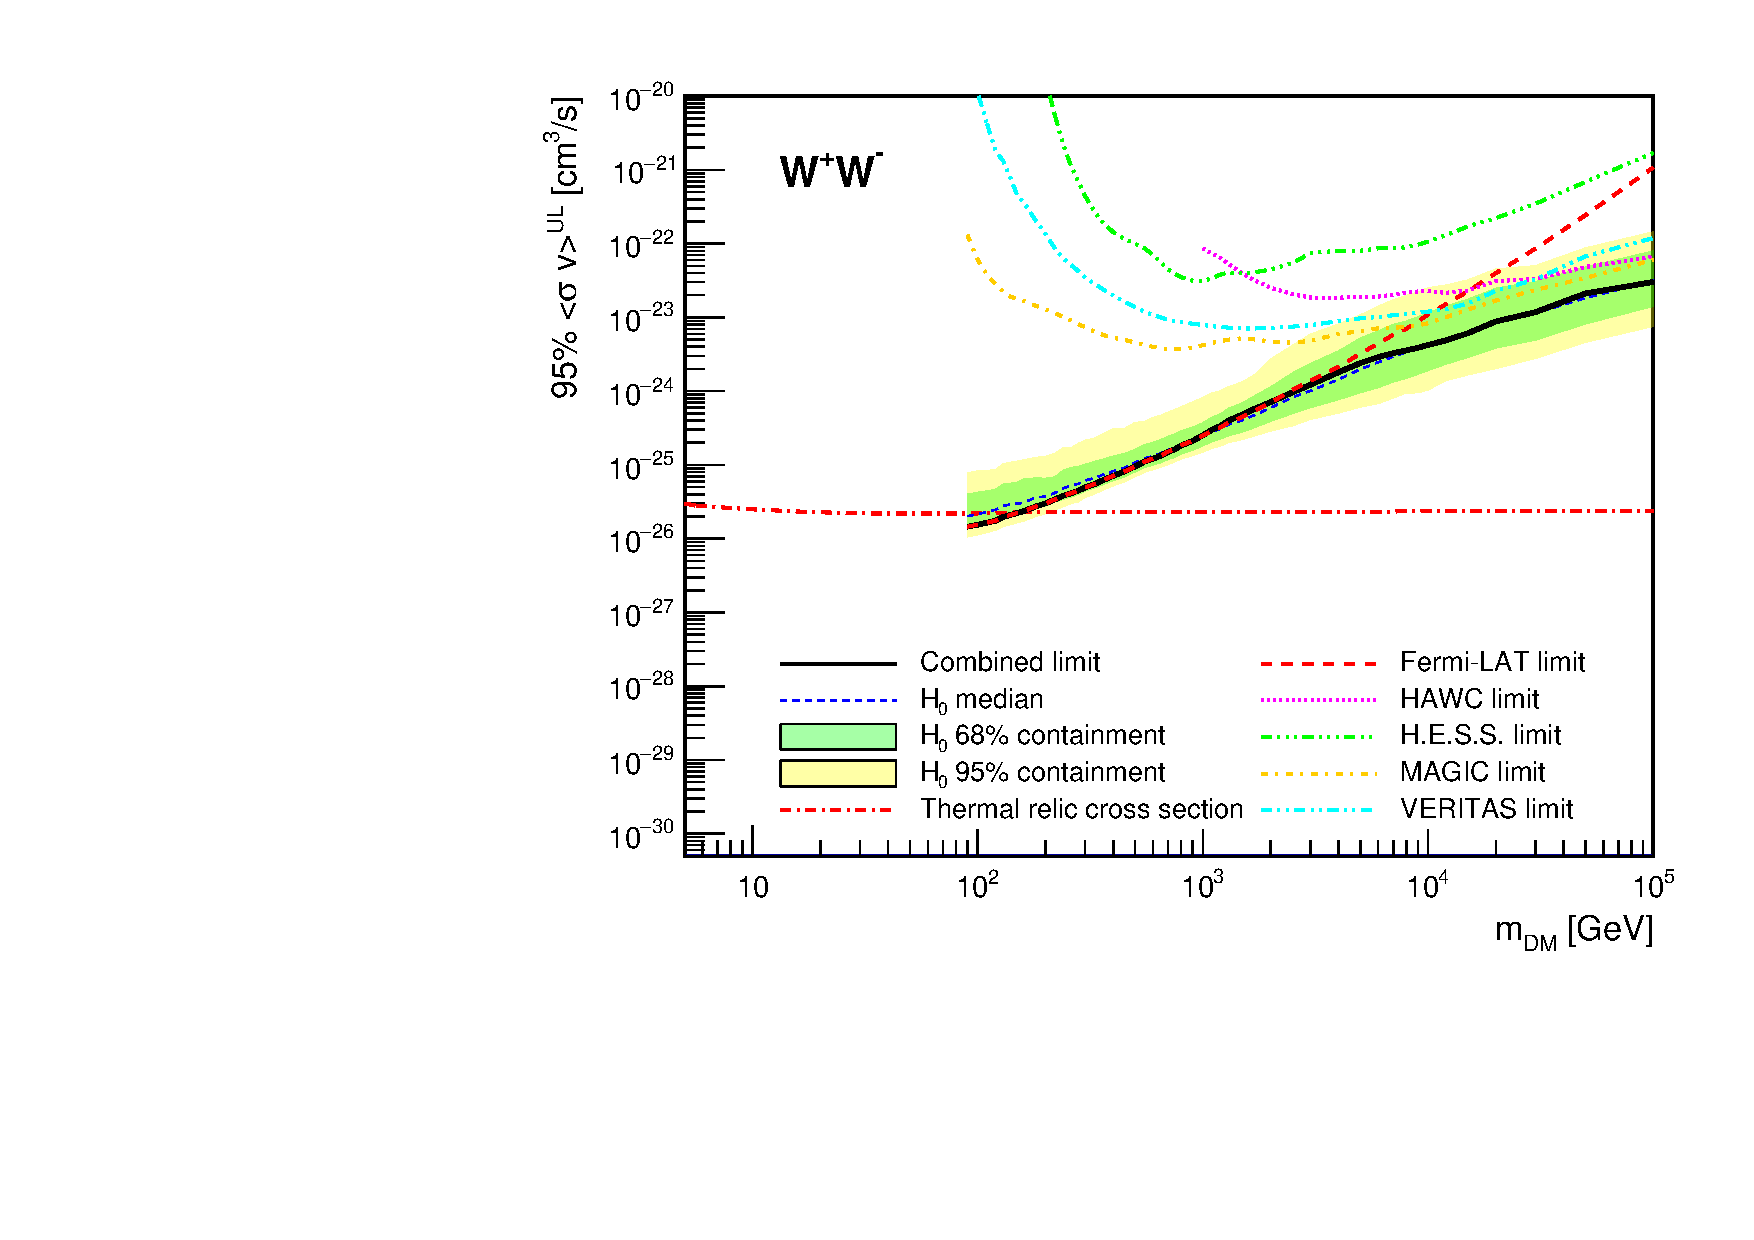
\includegraphics[width=0.35\textwidth]{figures/glory_duck/limits/Glory_Duck_Annihilation_WW_Geringer-Sameth_Combination_bands.pdf} &
        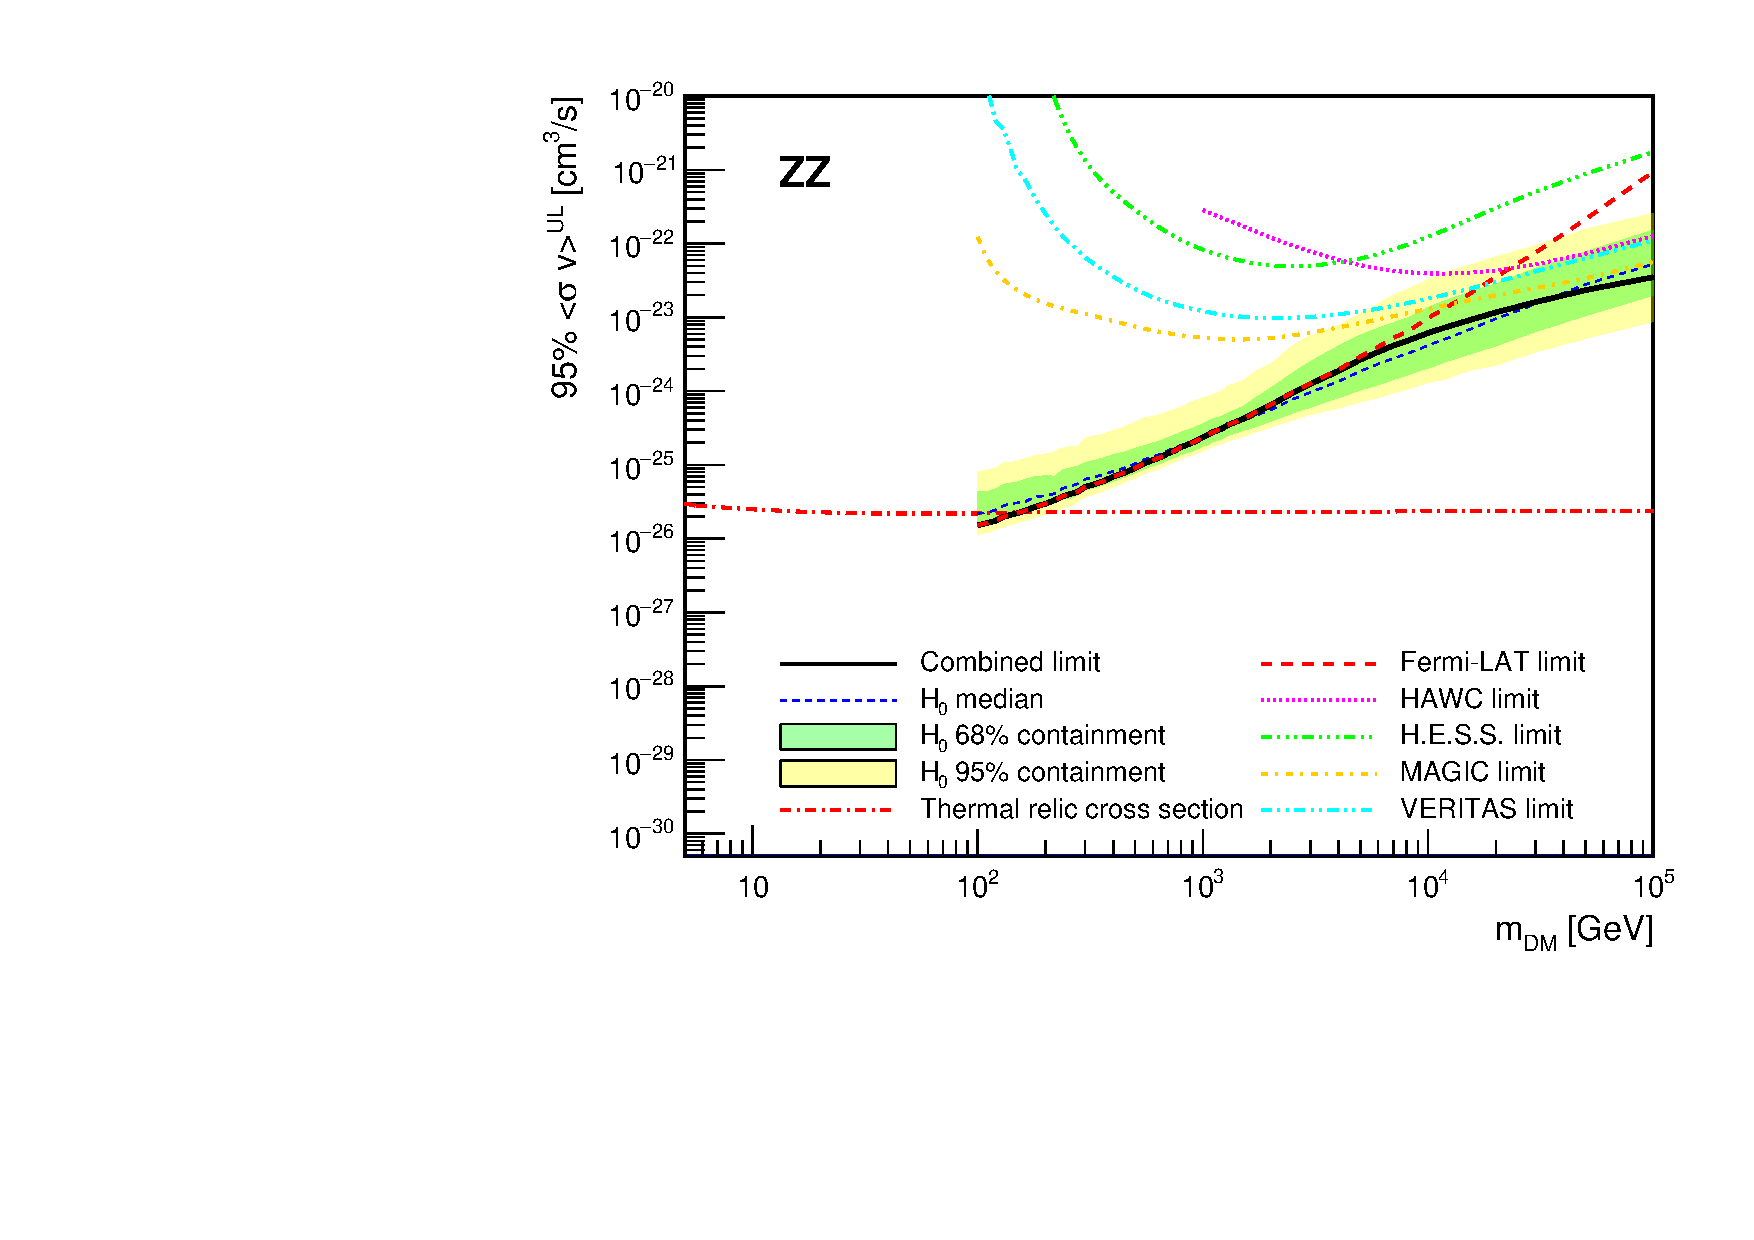
\includegraphics[width=0.35\textwidth]{figures/glory_duck/limits/Glory_Duck_Annihilation_ZZ_Geringer-Sameth_Combination_bands.pdf} \\
        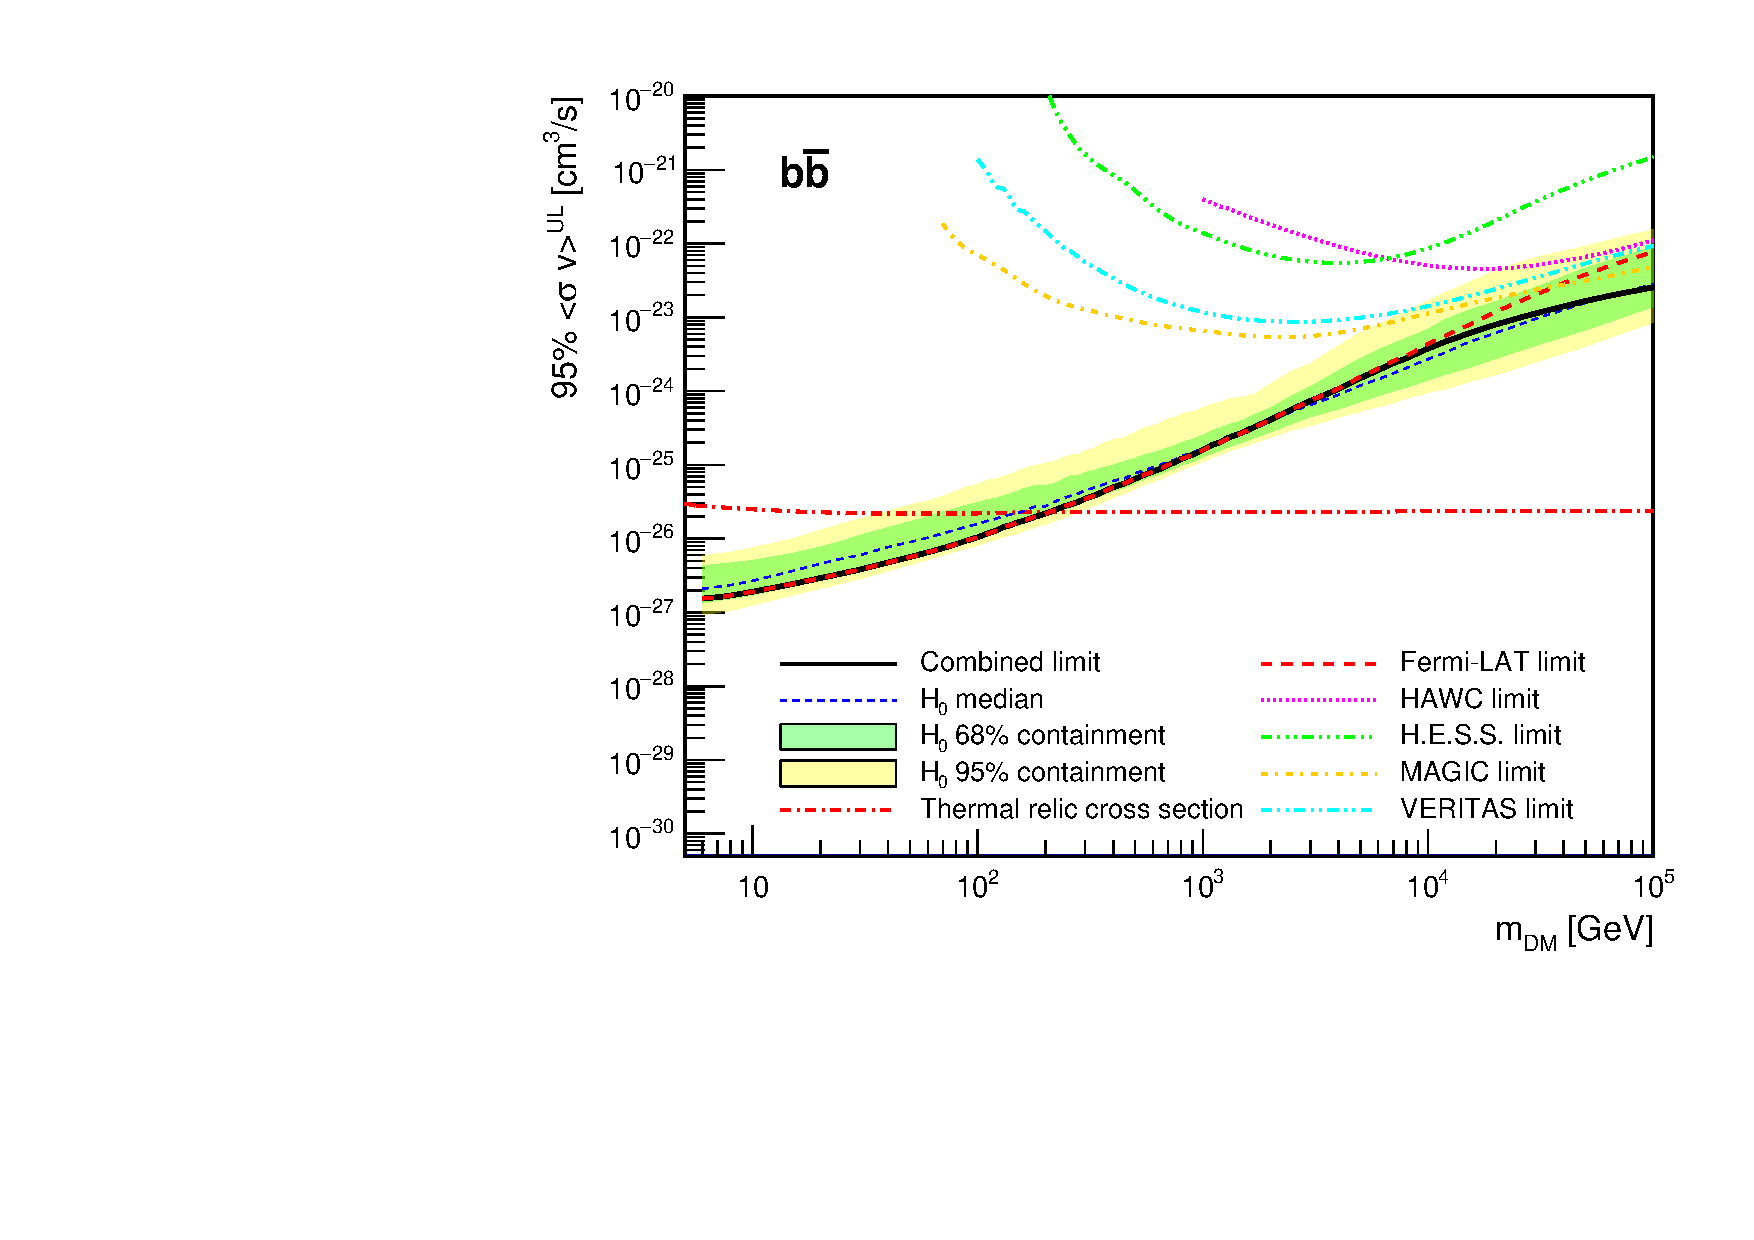
\includegraphics[width=0.35\textwidth]{figures/glory_duck/limits/Glory_Duck_Annihilation_bb_Geringer-Sameth_Combination_bands.pdf} &
        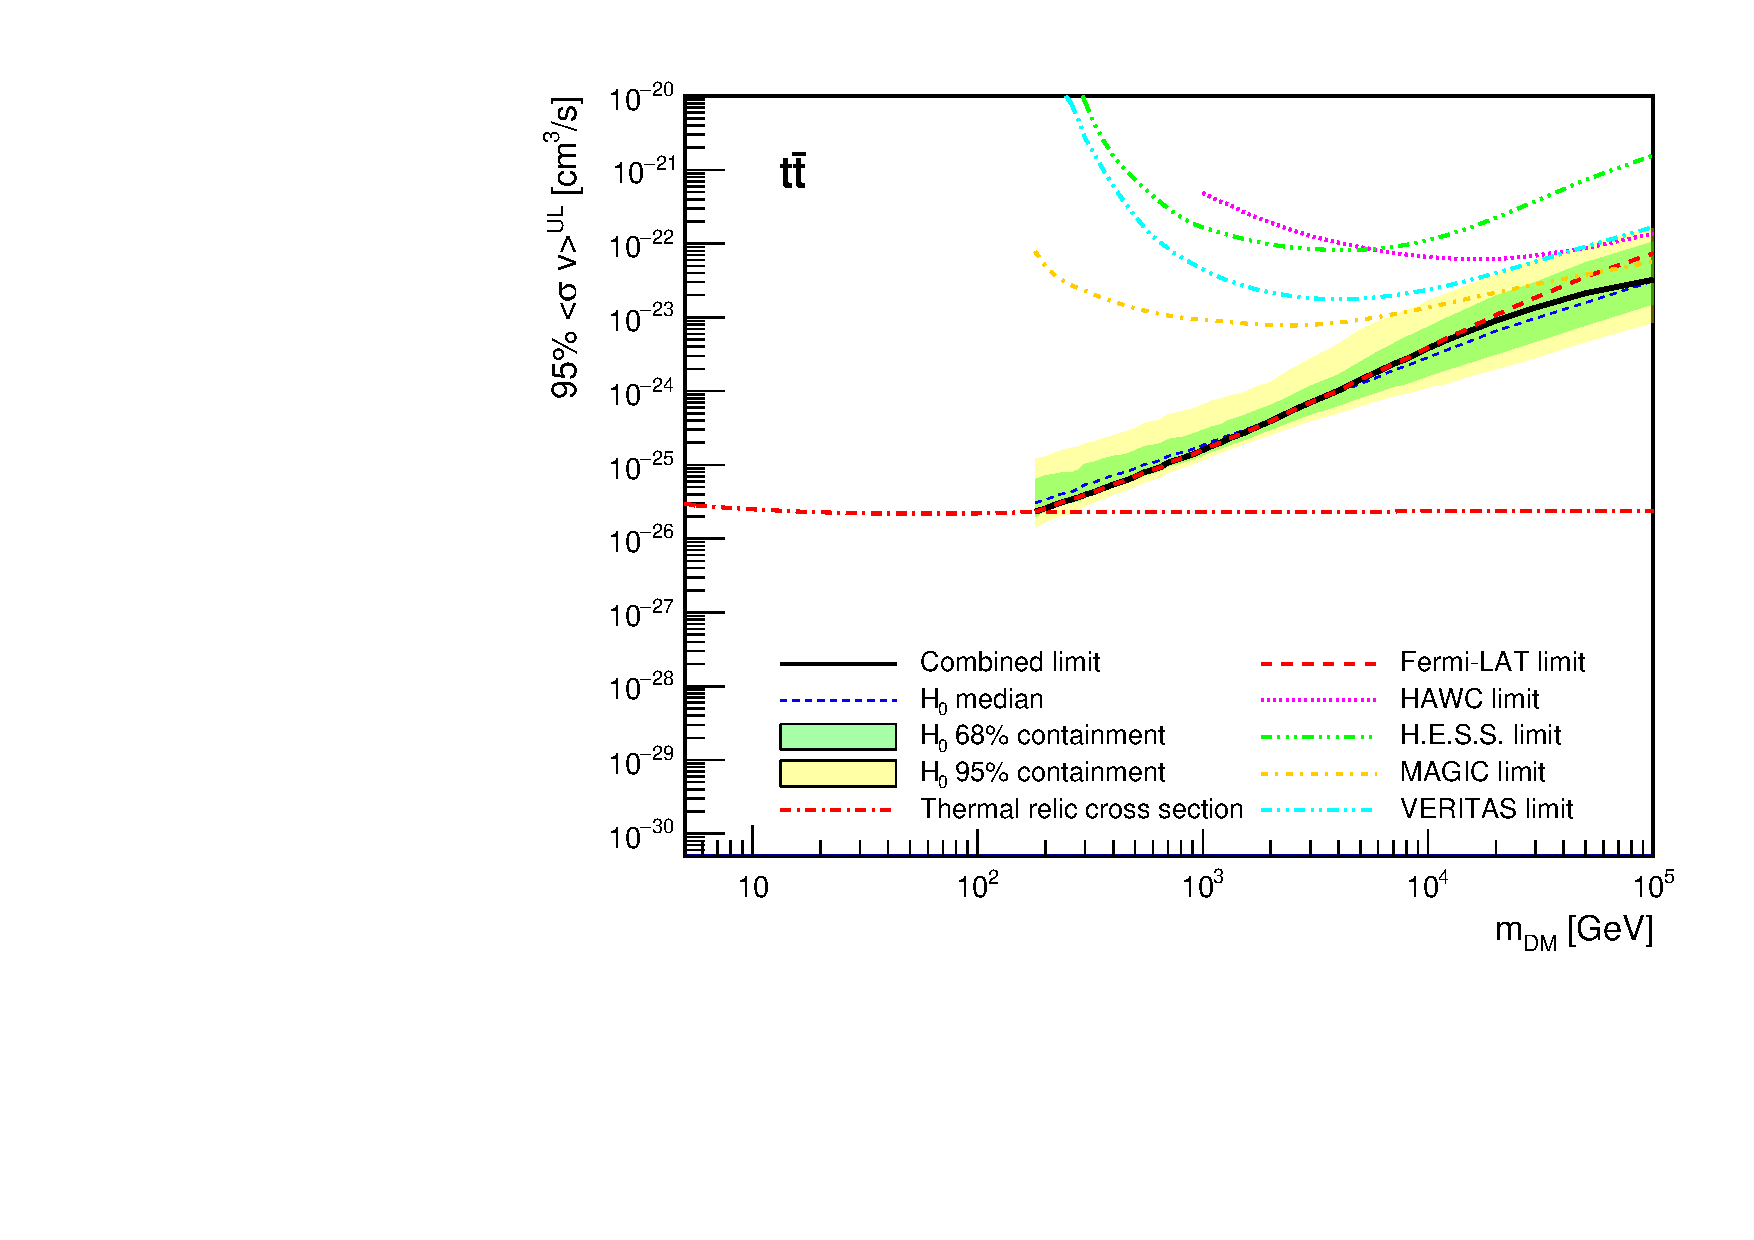
\includegraphics[width=0.35\textwidth]{figures/glory_duck/limits/Glory_Duck_Annihilation_tt_Geringer-Sameth_Combination_bands.pdf} \\
        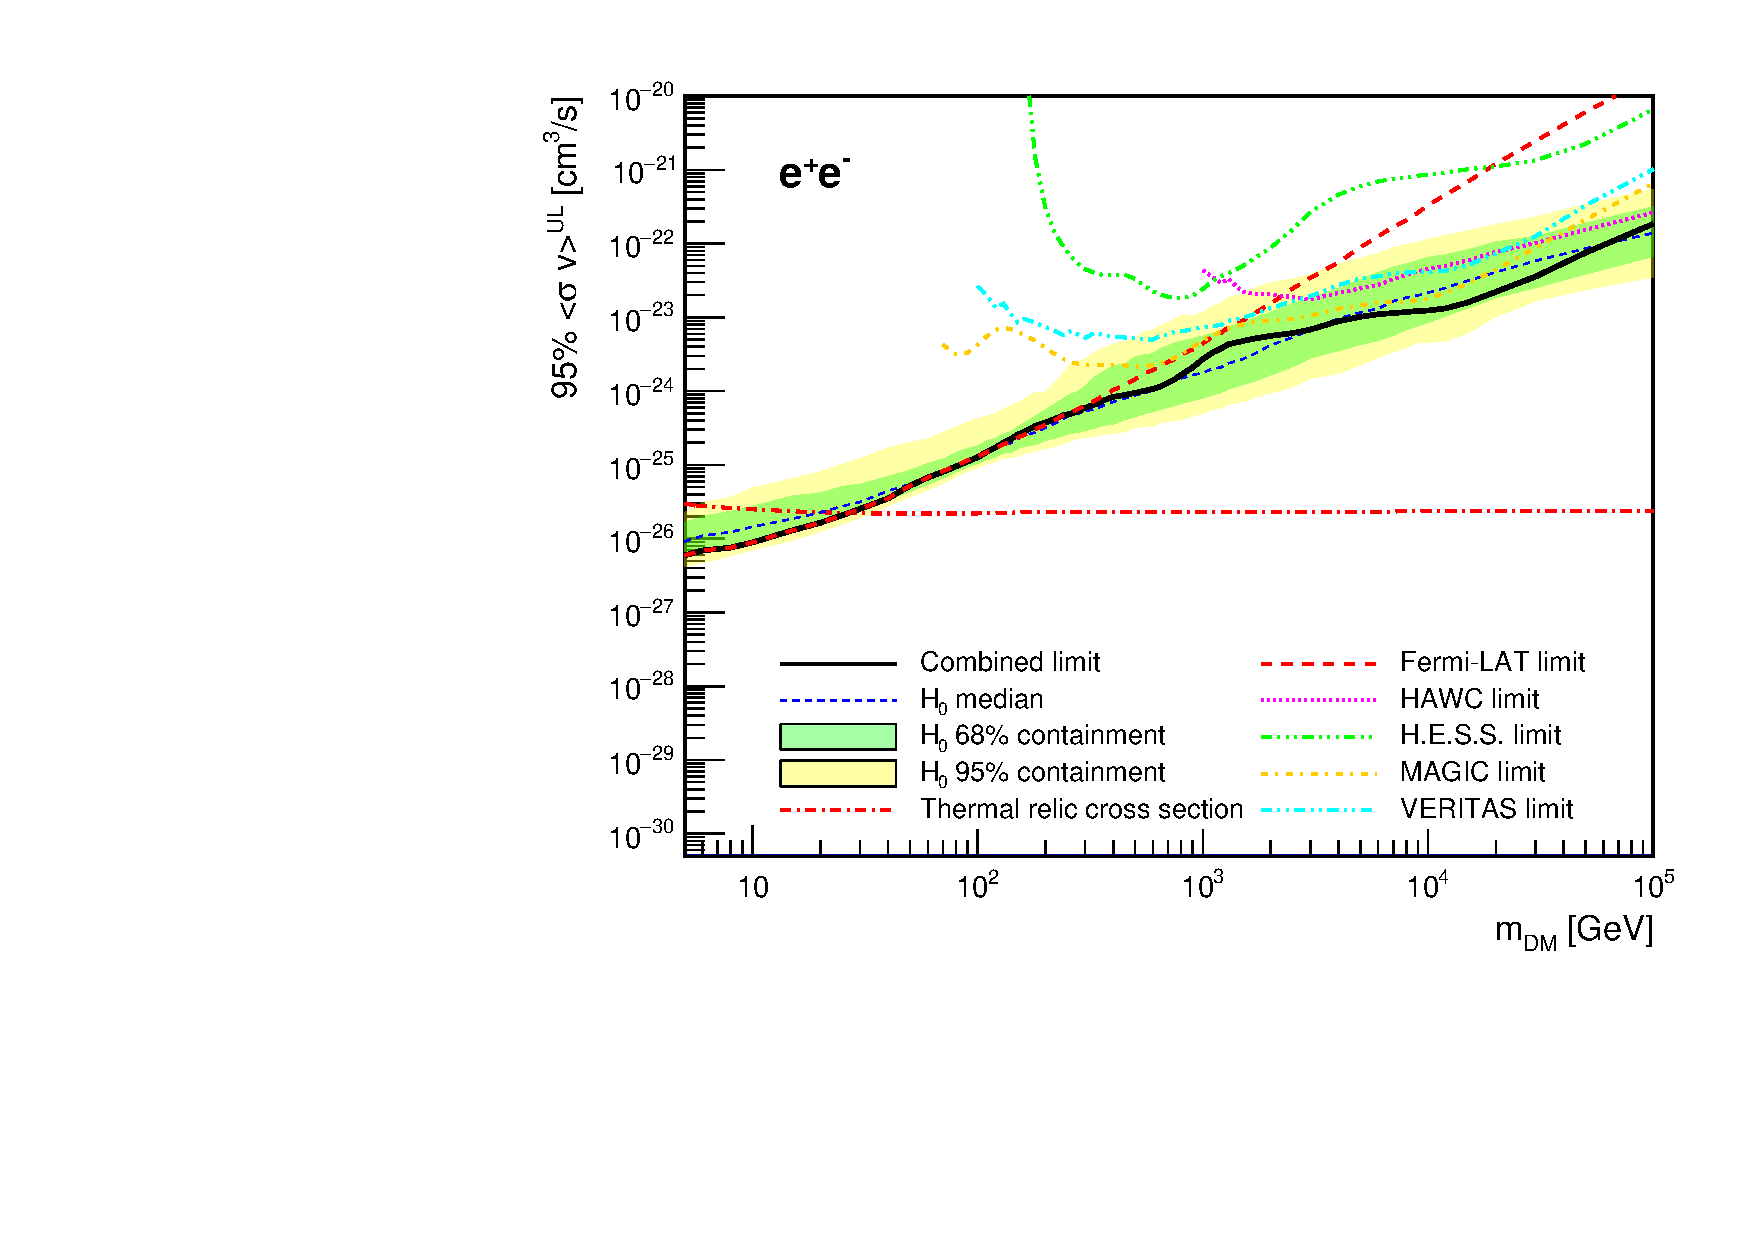
\includegraphics[width=0.35\textwidth]{figures/glory_duck/limits/Glory_Duck_Annihilation_ee_Geringer-Sameth_Combination_bands.pdf} &
        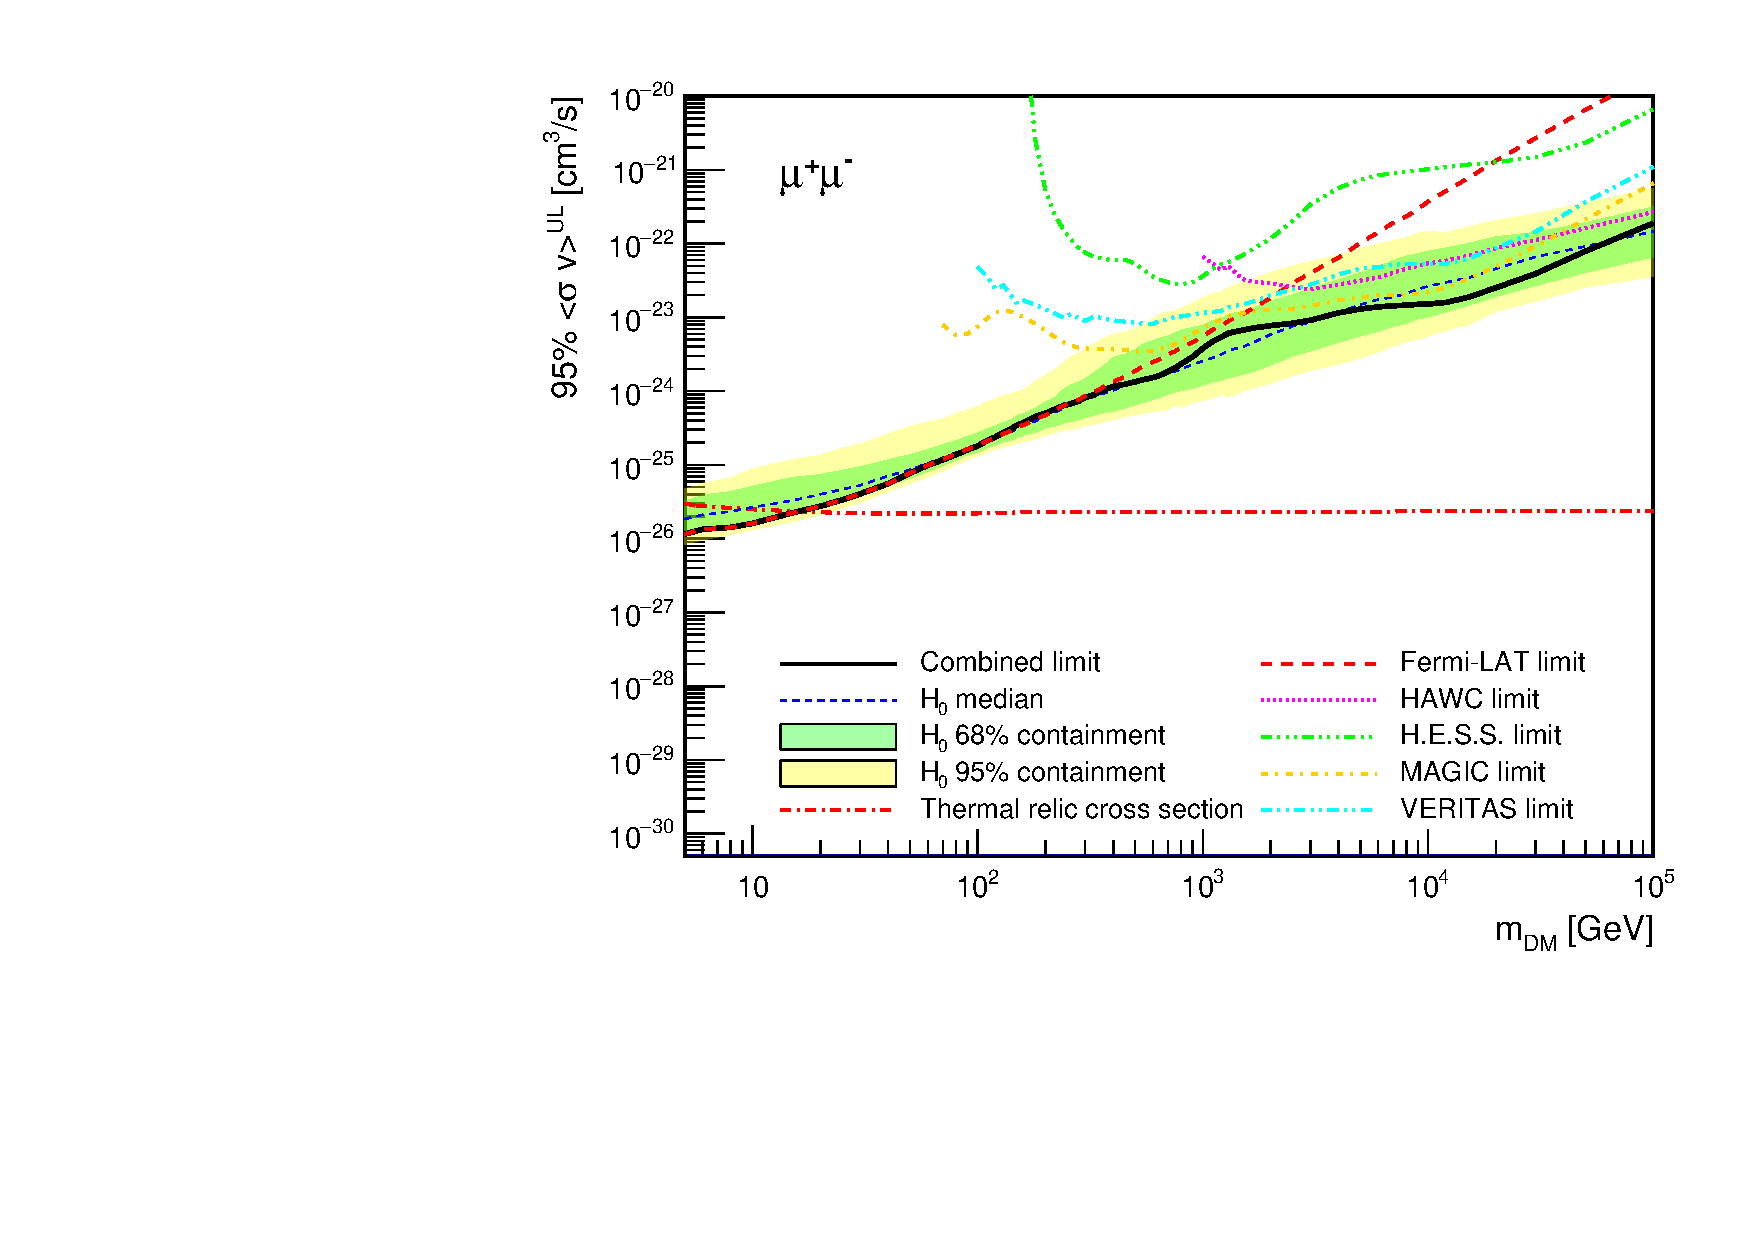
\includegraphics[width=0.35\textwidth]{figures/glory_duck/limits/Glory_Duck_Annihilation_mumu_Geringer-Sameth_Combination_bands.pdf} \\
        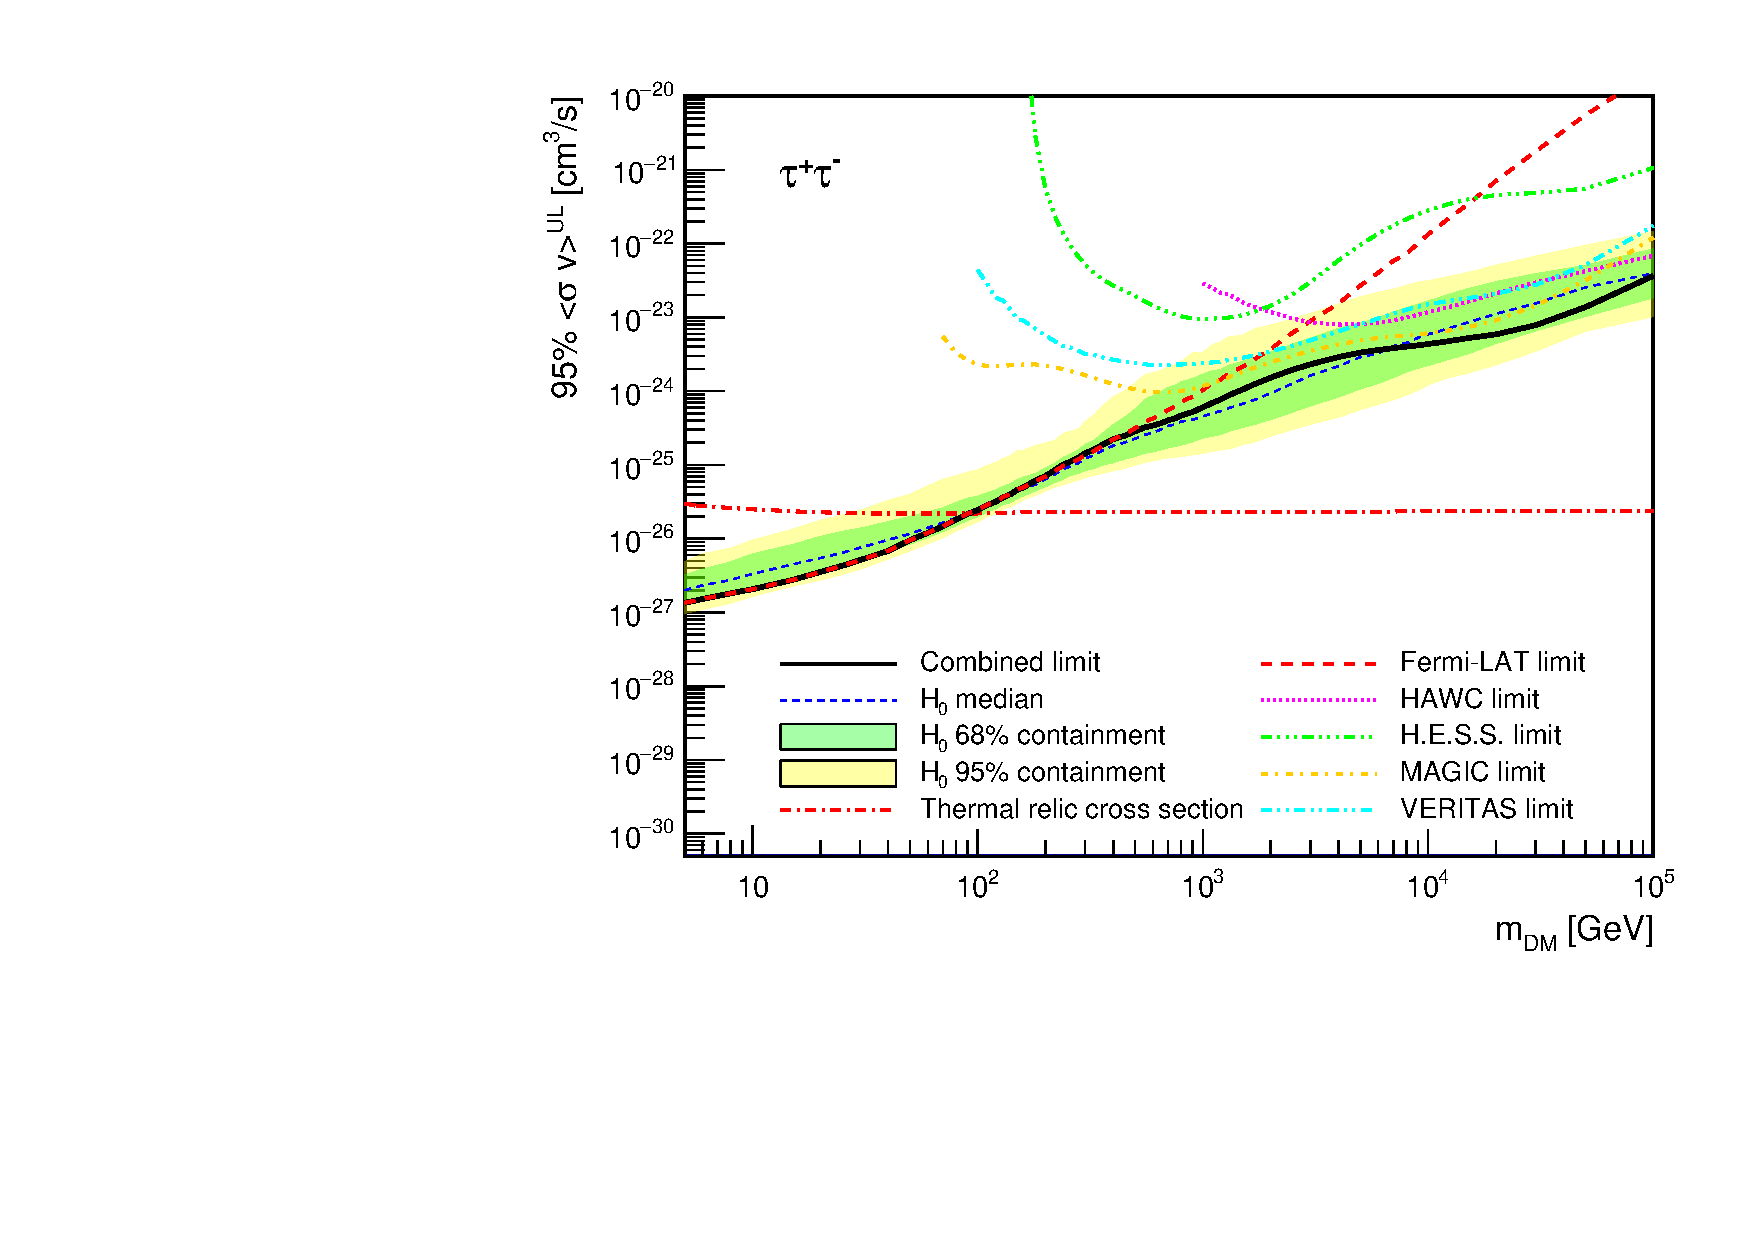
\includegraphics[width=0.35\textwidth]{figures/glory_duck/limits/Glory_Duck_Annihilation_tautau_Geringer-Sameth_Combination_bands.pdf} &
        \end{tabular}
        }
        \caption{Upper limits at 95\% confidence level on \sv in function of the DM mass for eight annihilation channels, using the set of \J factors from Ref.~\cite{Geringer-Sameth:2014yza} (\GS set in \Cref{tab:gd_J_factor}). The black solid line represents the observed combined limit, the black dashed line is the median of the null hypothesis corresponding to the expected limit, while the green and yellow bands show the 68\% and 95\% containment bands. Combined upper limits for each individual detector are also indicated as solid, colored lines.
        The value of the thermal relic cross-section in function of the DM mass is given as the red dotted-dashed line~\cite{Bertone_2005}.}
    \label{fig:limits-geringer-sameth}
    \end{figure}


    \begin{figure}[t]
    \centering{
    \begin{tabular}{cc}
        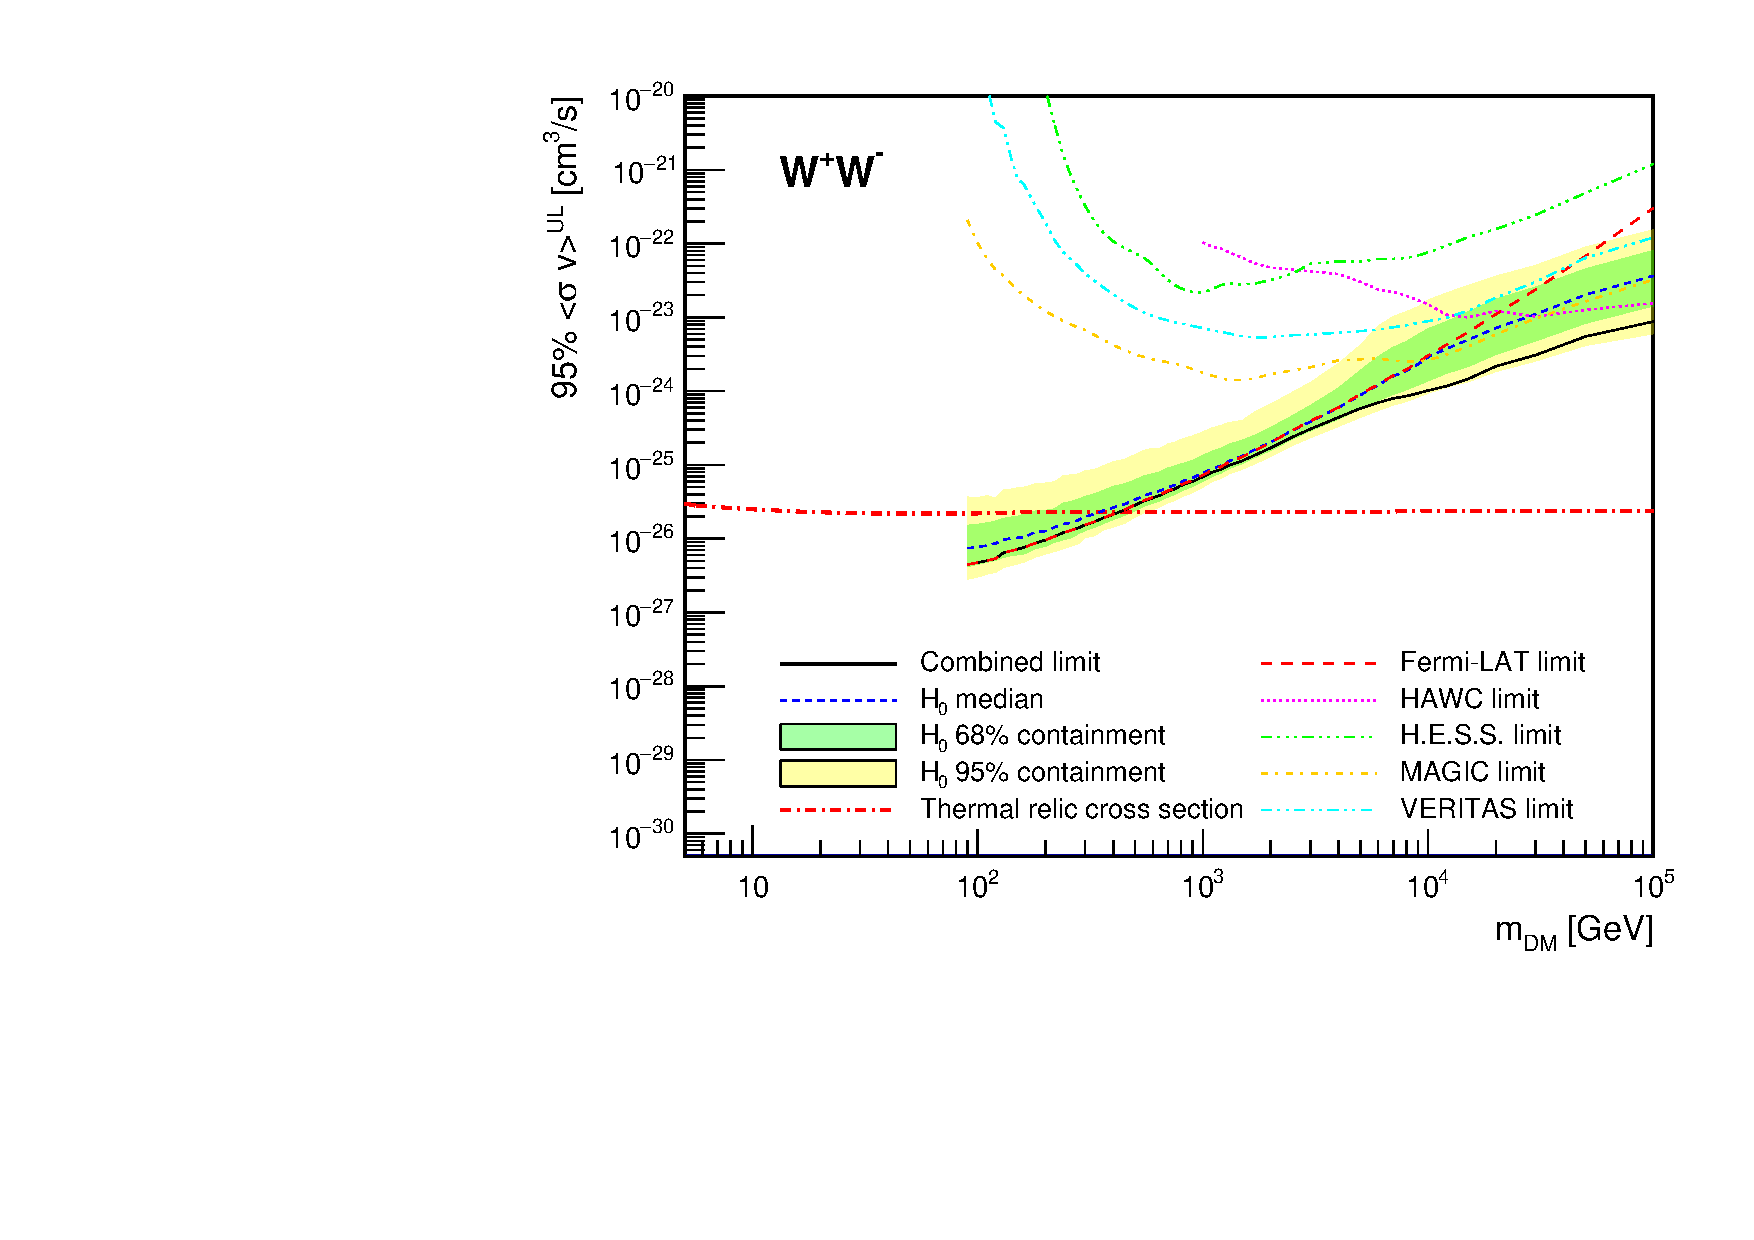
\includegraphics[width=0.35\textwidth]{figures/glory_duck/limits/Glory_Duck_Annihilation_WW_Bonnivard_Combination_bands.pdf} &
        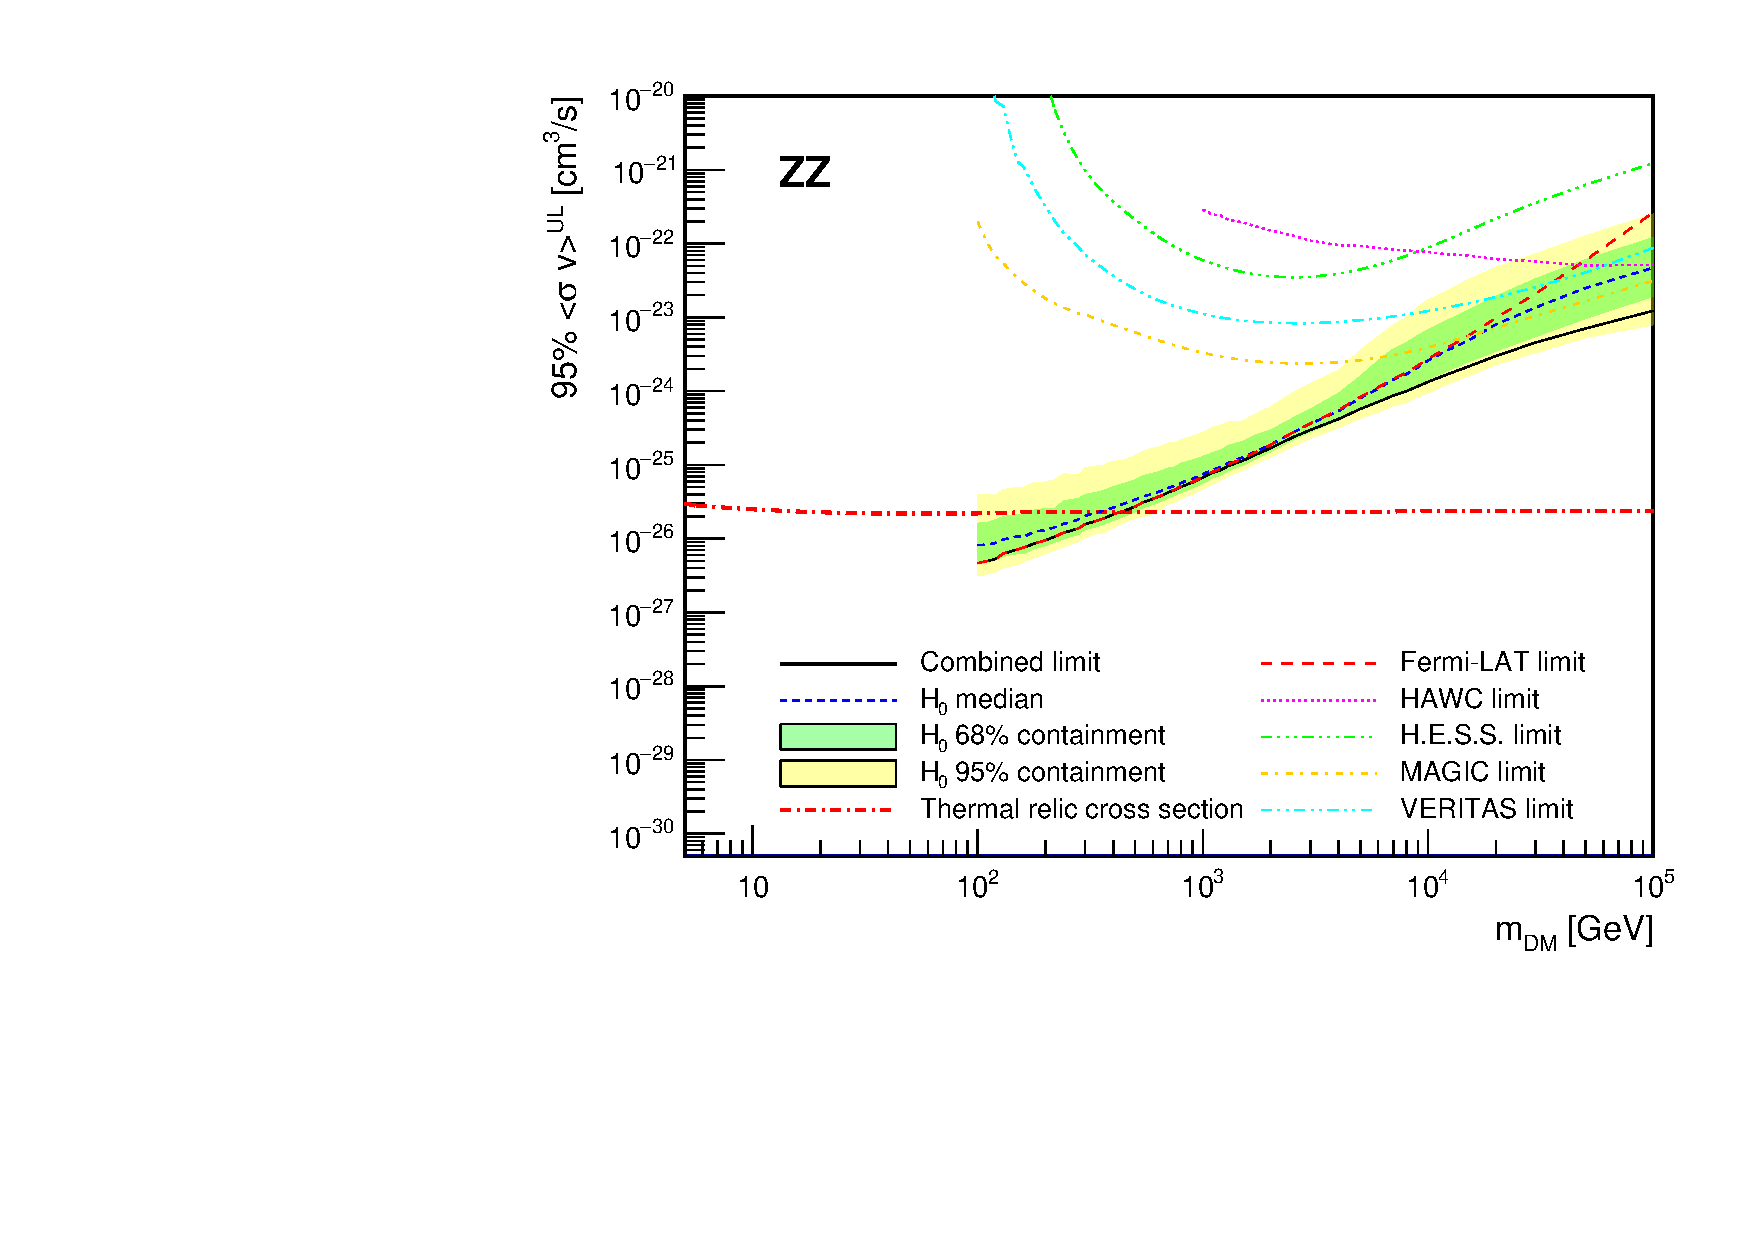
\includegraphics[width=0.35\textwidth]{figures/glory_duck/limits/Glory_Duck_Annihilation_ZZ_Bonnivard_Combination_bands.pdf} \\
        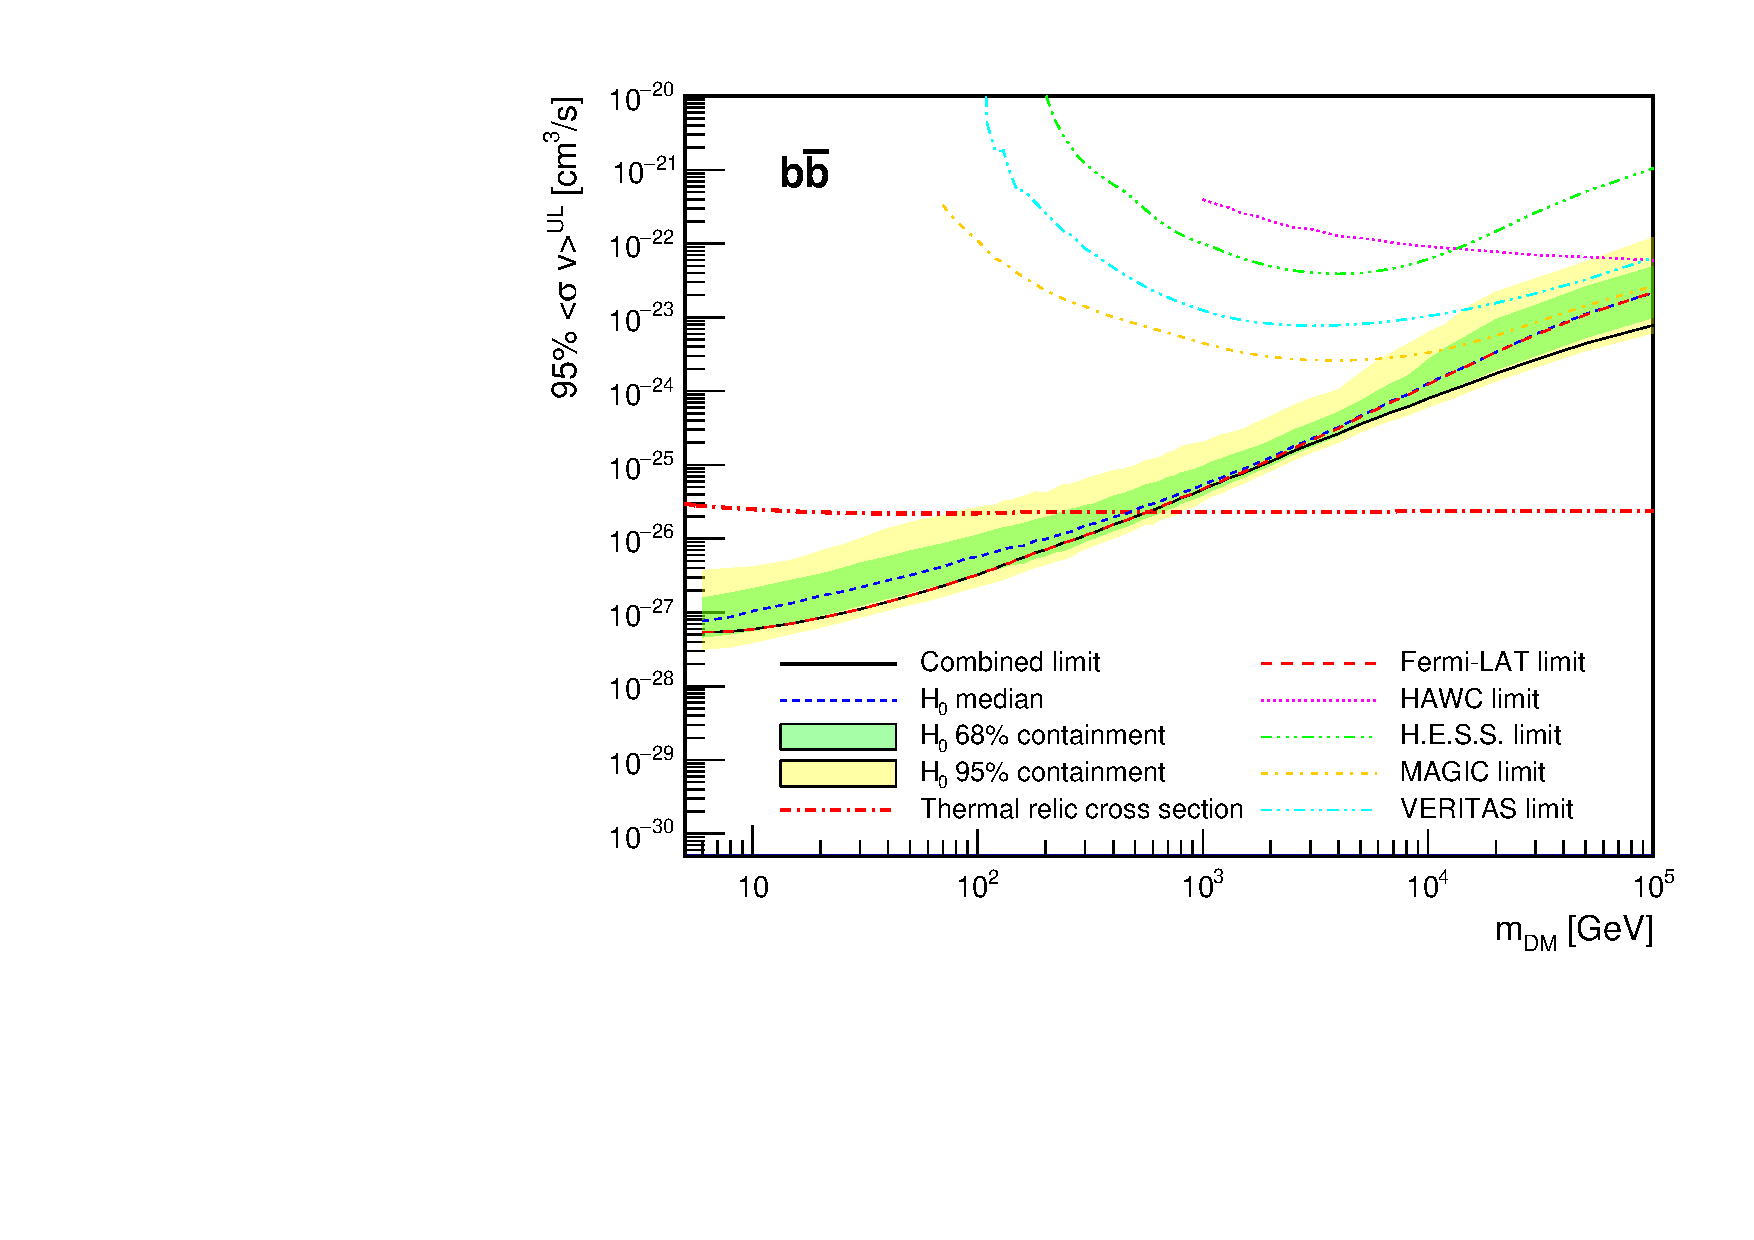
\includegraphics[width=0.35\textwidth]{figures/glory_duck/limits/Glory_Duck_Annihilation_bb_Bonnivard_Combination_bands.pdf} &
        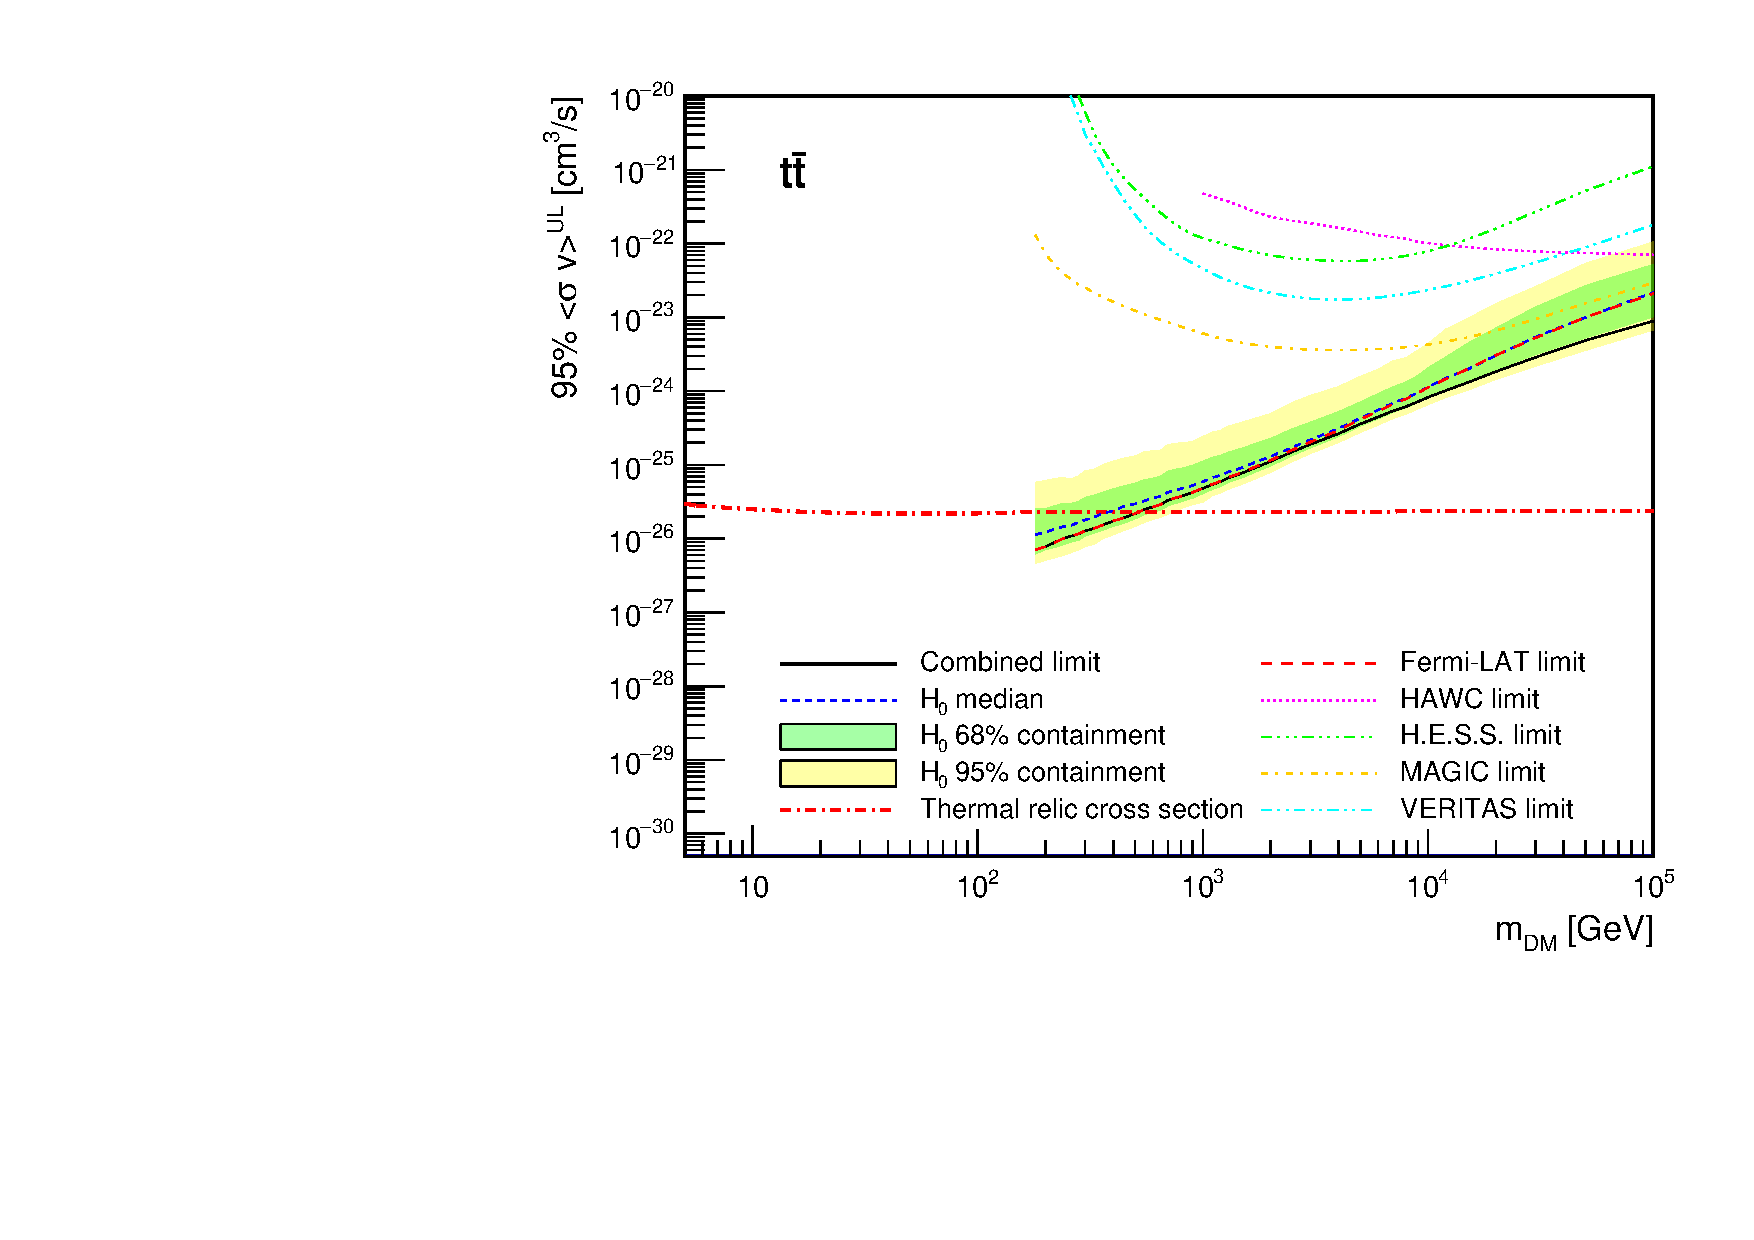
\includegraphics[width=0.35\textwidth]{figures/glory_duck/limits/Glory_Duck_Annihilation_tt_Bonnivard_Combination_bands.pdf} \\
        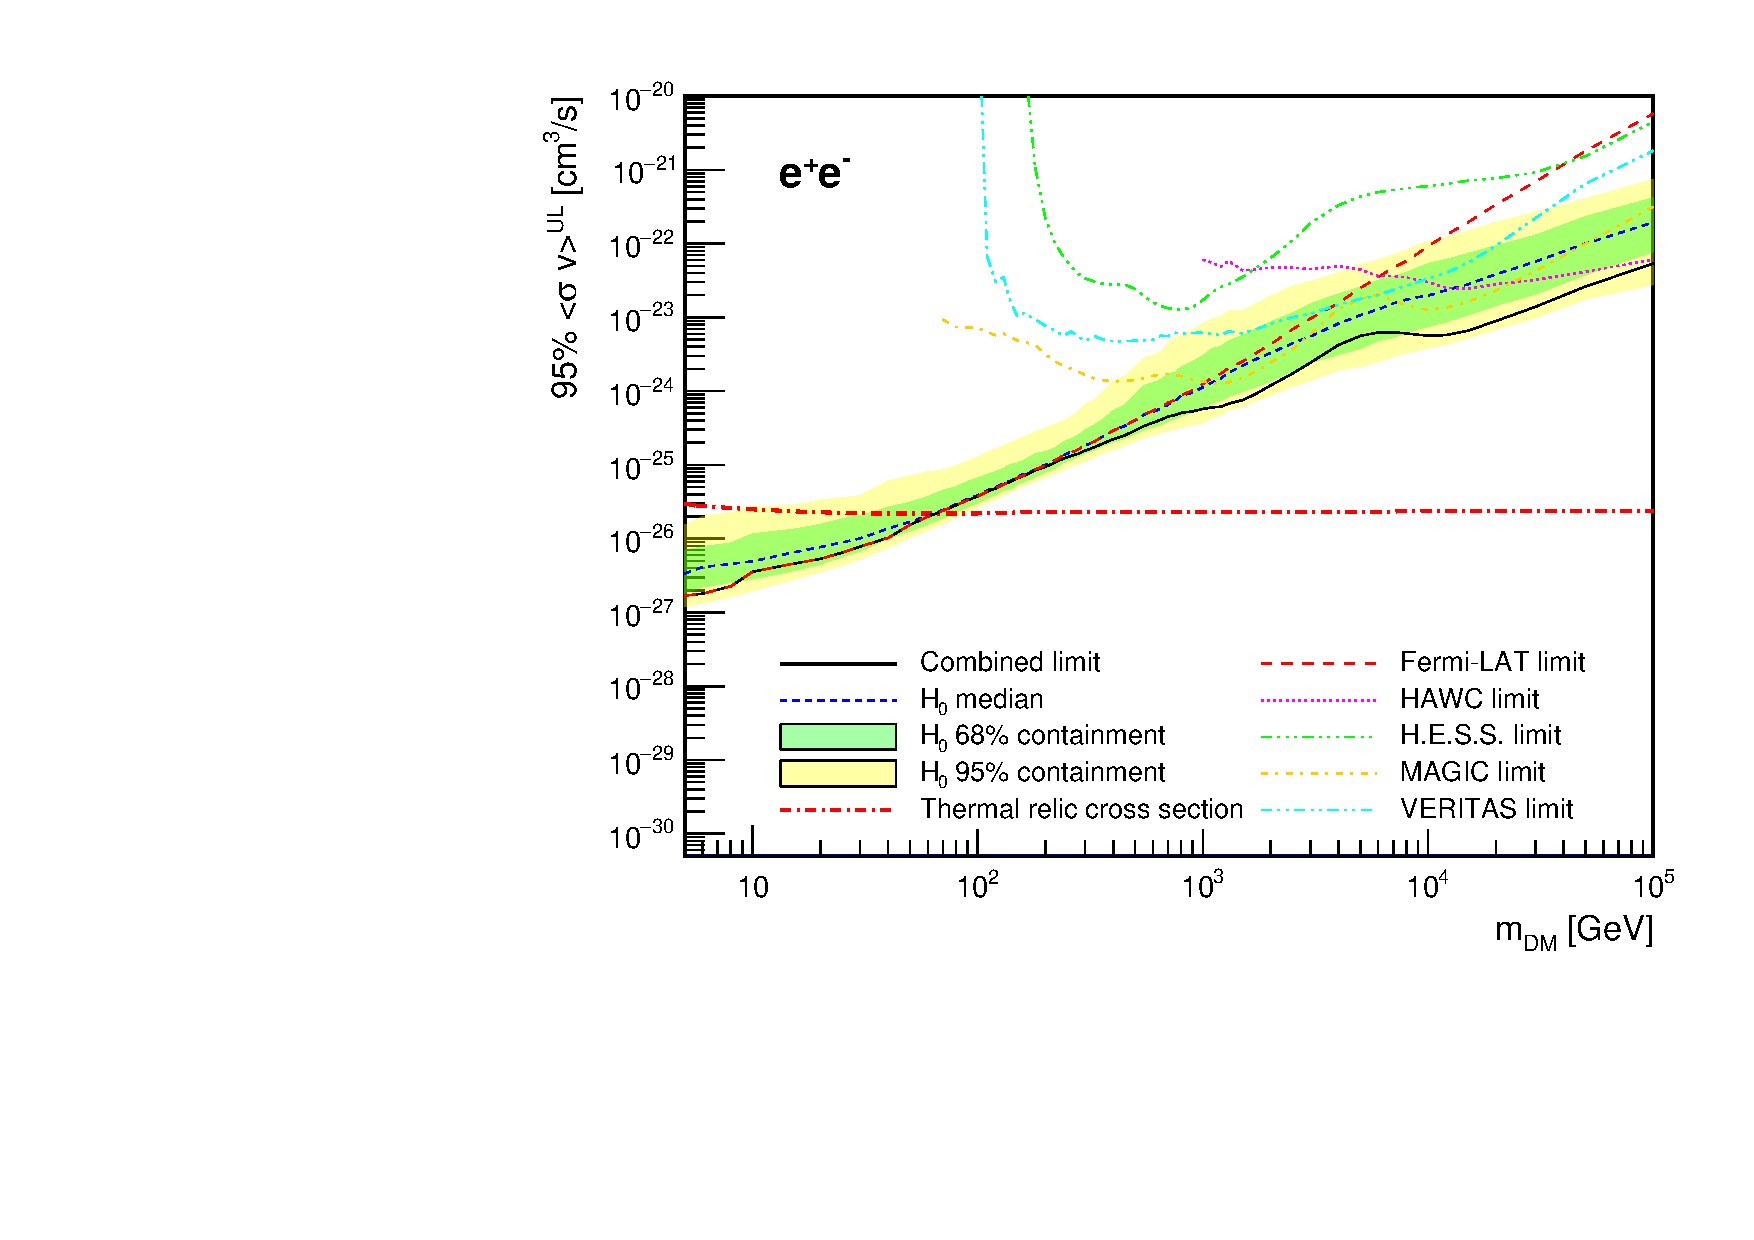
\includegraphics[width=0.35\textwidth]{figures/glory_duck/limits/Glory_Duck_Annihilation_ee_Bonnivard_Combination_bands.pdf} &
        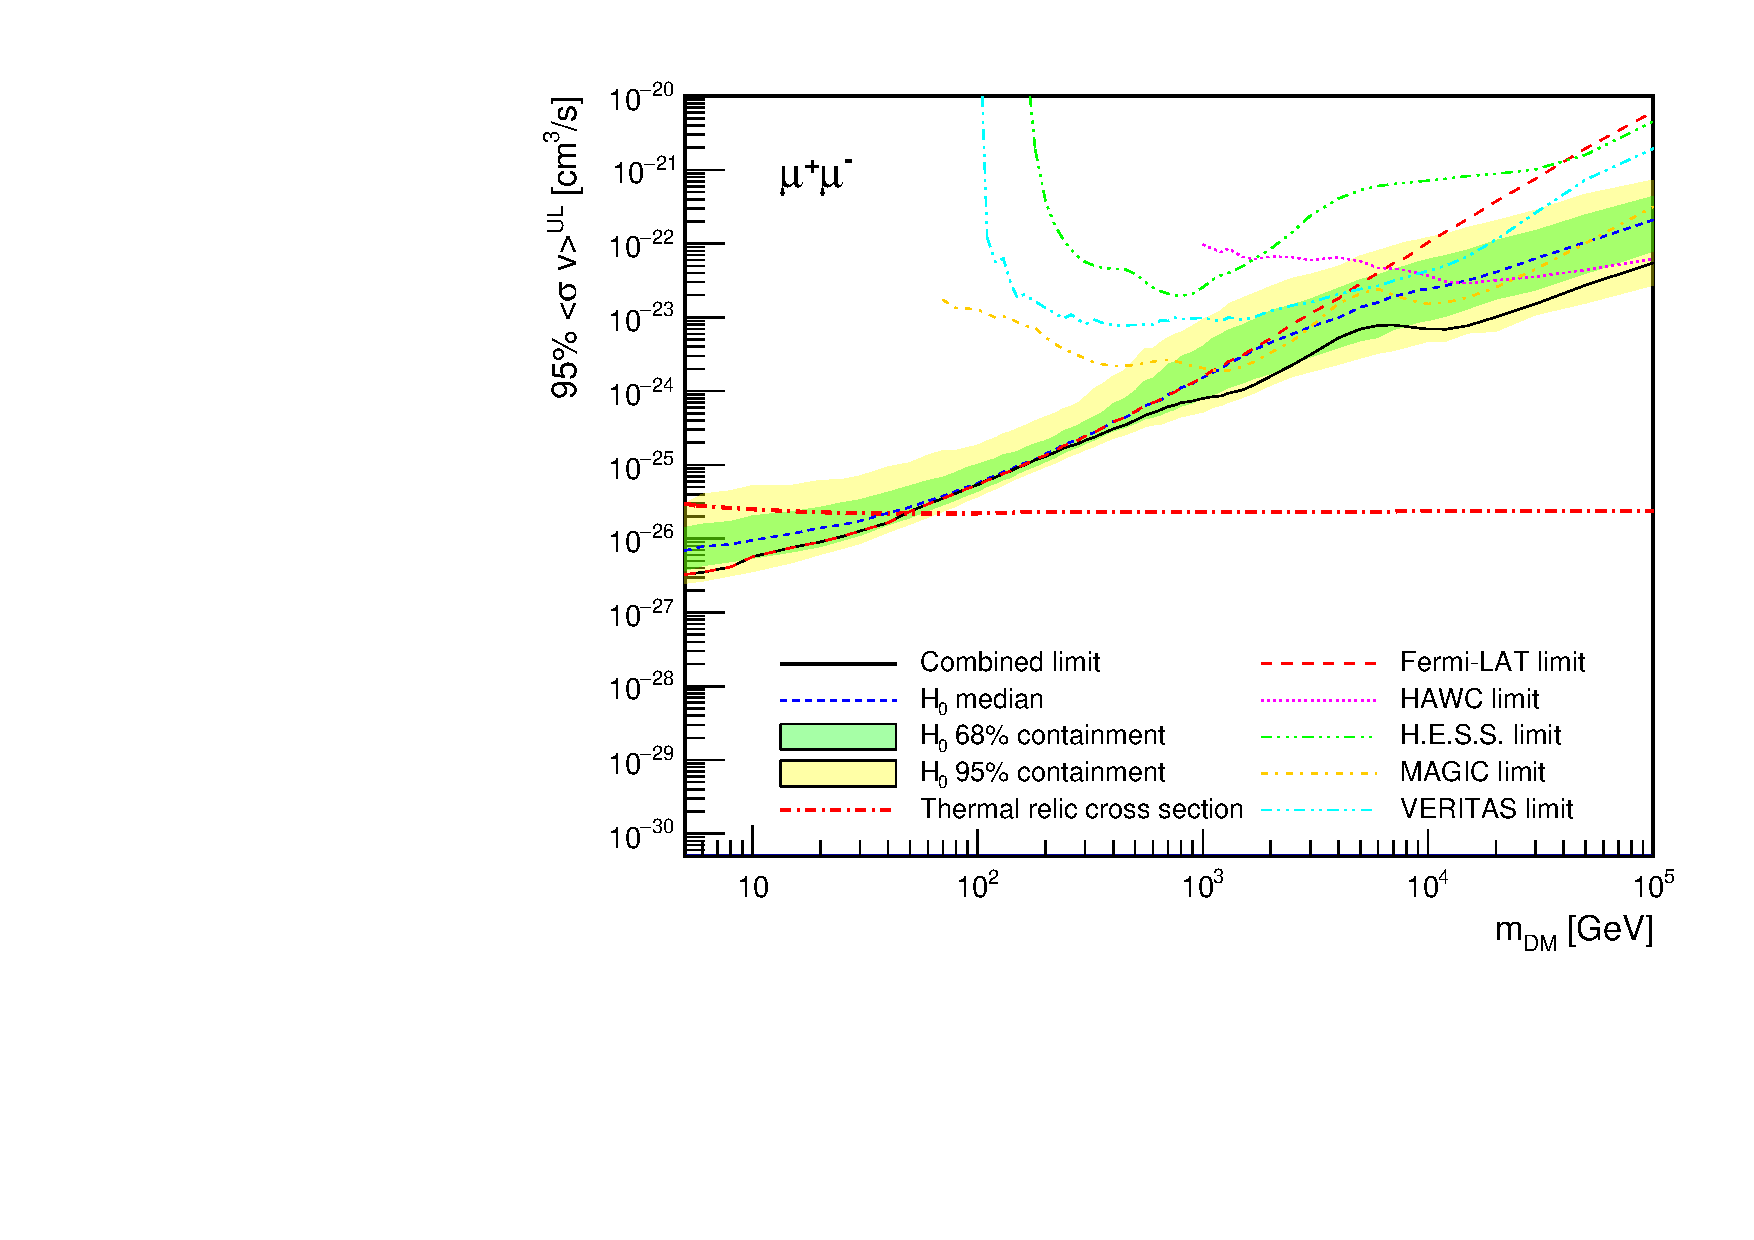
\includegraphics[width=0.35\textwidth]{figures/glory_duck/limits/Glory_Duck_Annihilation_mumu_Bonnivard_Combination_bands.pdf} \\
        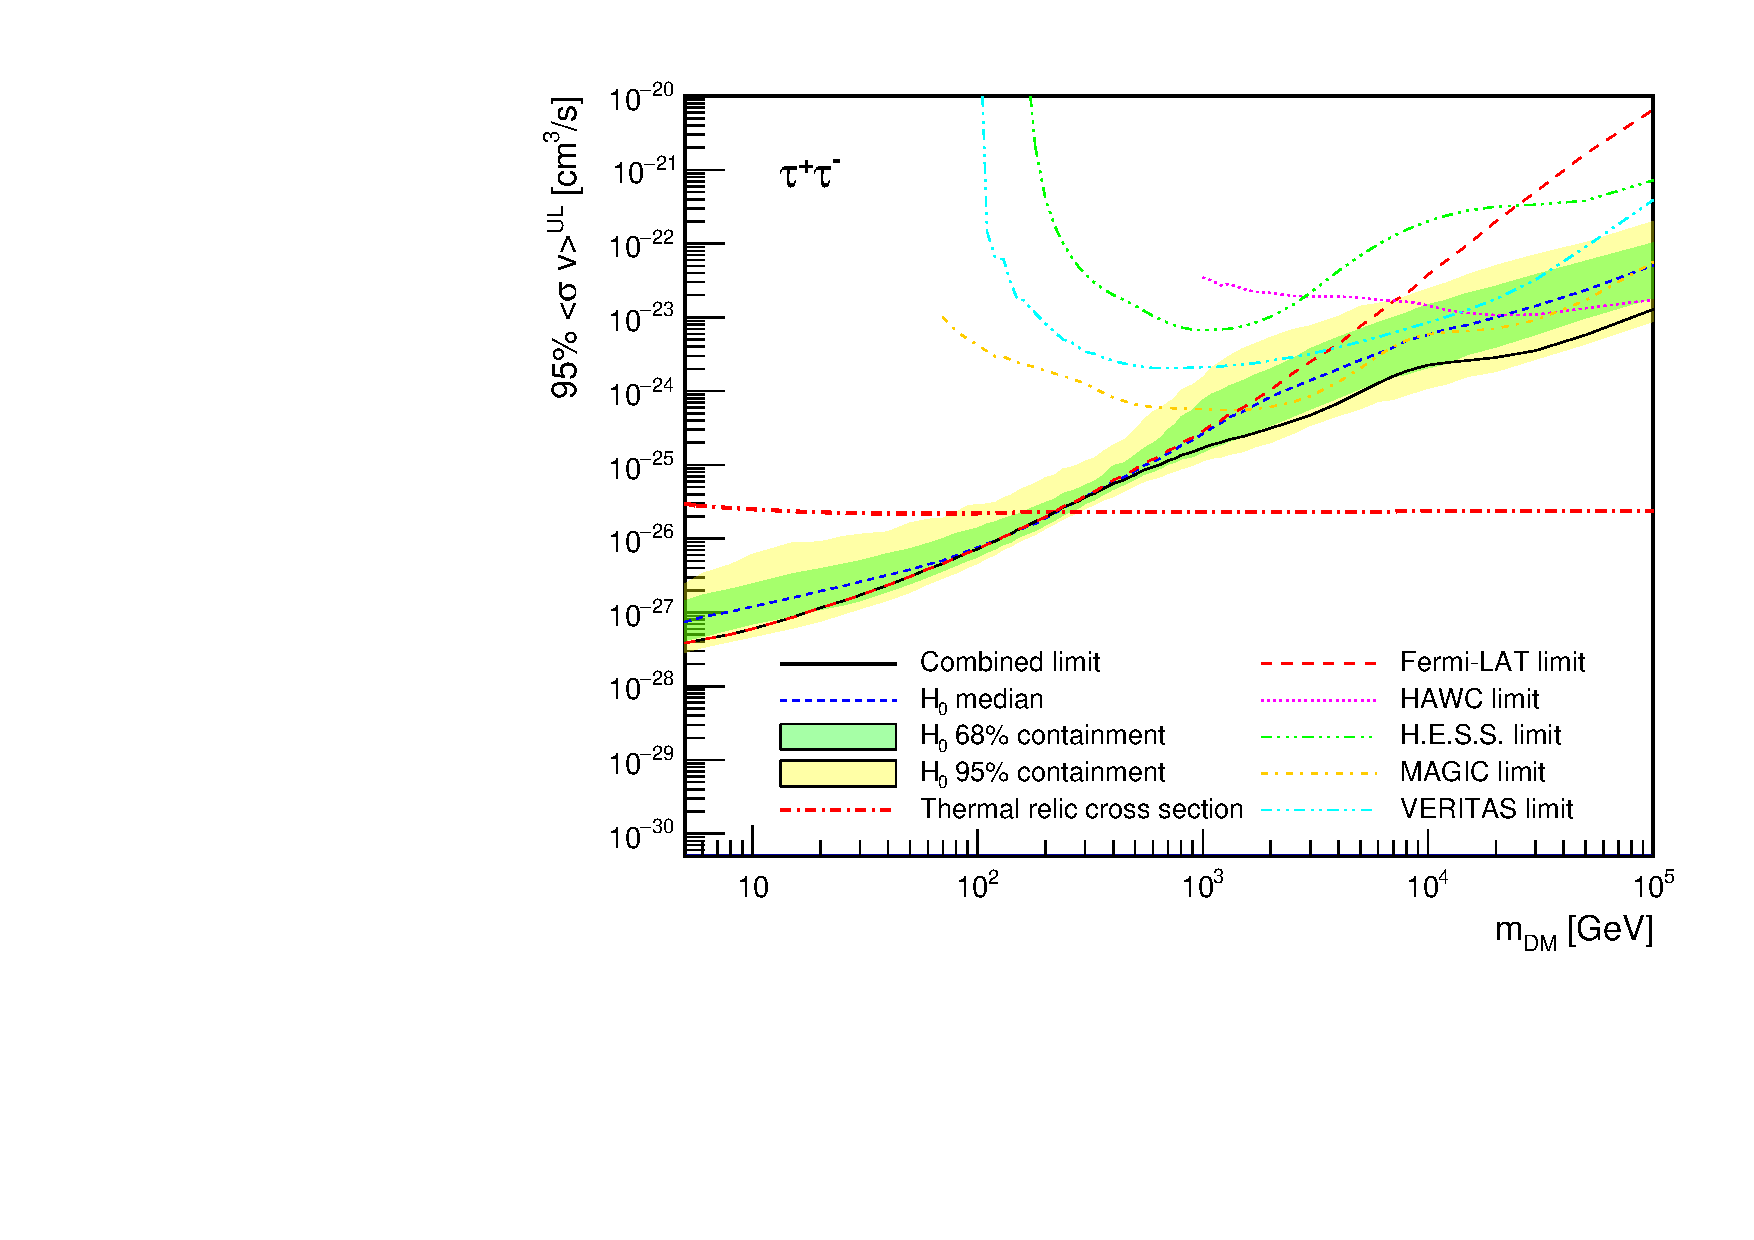
\includegraphics[width=0.35\textwidth]{figures/glory_duck/limits/Glory_Duck_Annihilation_tautau_Bonnivard_Combination_bands.pdf} &
        \end{tabular}
        }
        \caption{Same as \cref{fig:limits-geringer-sameth}, using the set of \J factors from Ref.~\cite{Bonnivard:2014kza, Bonnivard:2015xpq} (\B set in \Cref{tab:gd_J_factor}).}
    \label{fig:limits-bonnivard}
    \end{figure}

The crux of this analysis is that HAWC's results are combined with 4 other gamma-ray observatories: Fermi-LAT, H.E.S.S., MAGIC, and VERITAS.
\sloppy No significant DM emission was observed by any of the five instruments.
We present the upper limits on \sv assuming seven independent DM self annihilation channels, namely $W^+W^-$, $Z^+Z^-$, $b\bar{b}$, $t\bar{t}$, $e^+e^-$, $\mu^+\mu^-$, and $\tau^+\tau^-$.
The 68\% and 95\% containment bands are produced from 300 Poisson realizations of the null hypothesis corresponding to each of the combined datasets.
These 300 realizations are combined identically to dSph observations.
The containment bands and the median are extracted from the distribution of resulting limits on the null hypothesis.
These 300 realizations are obtained either by fast simulations of the OFF observations, for H.E.S.S., MAGIC, VERITAS, and HAWC, or taken from real observations of empty fields of view in the case of Fermi-LAT~\cite{2015PhRvL.115w1301A,Fermi-LAT:2016uux,2021PhRvD.103l3005D}.

The obtained limits are shown in \Cref{fig:limits-geringer-sameth} for the \GS set of \J-factors~\cite{Geringer-Sameth:2014yza} and in \Cref{fig:limits-bonnivard} for the \B set of \J-factors~\cite{Bonnivard:2014kza, Bonnivard:2015xpq}.
The combined limits are presented with their 68\% and 95\% containment bands, and are expected to be close to the median limit when no signal is present.
We observe agreement with the null hypothesis for all channels, within $2\sigma$ standard deviations, between the observed limits and the expectations given by the median limits.
Limits obtained from each detector are also indicated in the figures, where limits for all dSphs observed by the specific instrument have been combined.

Below \textasciitilde300 GeV, the $Fermi$-LAT dominates the DM limits for all annihilation channels.
From \textasciitilde300 GeV to \textasciitilde2 TeV, $Fermi$-LAT continues to dominate for the hadronic and bosonic DM channels, yet the IACTs (H.E.S.S., MAGIC, and VERITAS) and $Fermi$-LAT all contribute to the limit for leptonic DM channels.
For DM masses between \textasciitilde2 TeV to \textasciitilde10 TeV, the IACTs dominate leptonic DM annihilation channels, whereas both the $Fermi$-LAT and the IACTs dominate bosonic and hadronic DM annihilation channels.
From \textasciitilde10 TeV to \textasciitilde100 TeV, both the IACTs and HAWC contribute significantly to the leptonic DM limit.
For hadronic and bosonic DM, the IACTs and $Fermi$-LAT both contribute strongly.

We notice that the limits computed using the \B set of \J-factor are always better compared to the ones calculated with the \GS set.
For the $W^+W^-$, $Z^+Z^-$, $b\bar{b}$, and $t\bar{t}$ channels, the ratio between the limits computed with the two sets of \J-factor is varying between a factor of \textasciitilde3 and \textasciitilde5 depending on the energy, with the largest ratio around 10~TeV.
For the channels $e^+e^-$, $\mu^+\mu^-$, and $\tau^+\tau^-$, the ratio lies between \textasciitilde2 to \textasciitilde6, being maximum around 1~TeV.
Examining \Cref{fig:comparison_J_1} and \Cref{fig:comparison_J_2} in \Cref{sec:gd_jfactor_systematic}, these differences are explained by the fact that the \B set provides higher \J-factors for the majority of the studied dSphs, with the notable exception of Segue~I.
The variation on the ratio of the limits for the two sets is due to different dSph dominating the limits depending on the energy.
One set, \B, pushes the range of which thermal cross-section which can be excluded to higher mass.
This comparison demonstrates the magnitude of systematic uncertainties associated with the choice of the \J-factor calculation
The \GS and \B sets present a difference in the limits for all channels of about
This difference is explained, see  \Cref{fig:comparison_J_1} and \Cref{fig:comparison_J_2}, by the fact that the \B set provides higher \J-factors for all dSph except for Segue~I.

\begin{figure}[t]
\centering{
\begin{tabular}{ccc}
    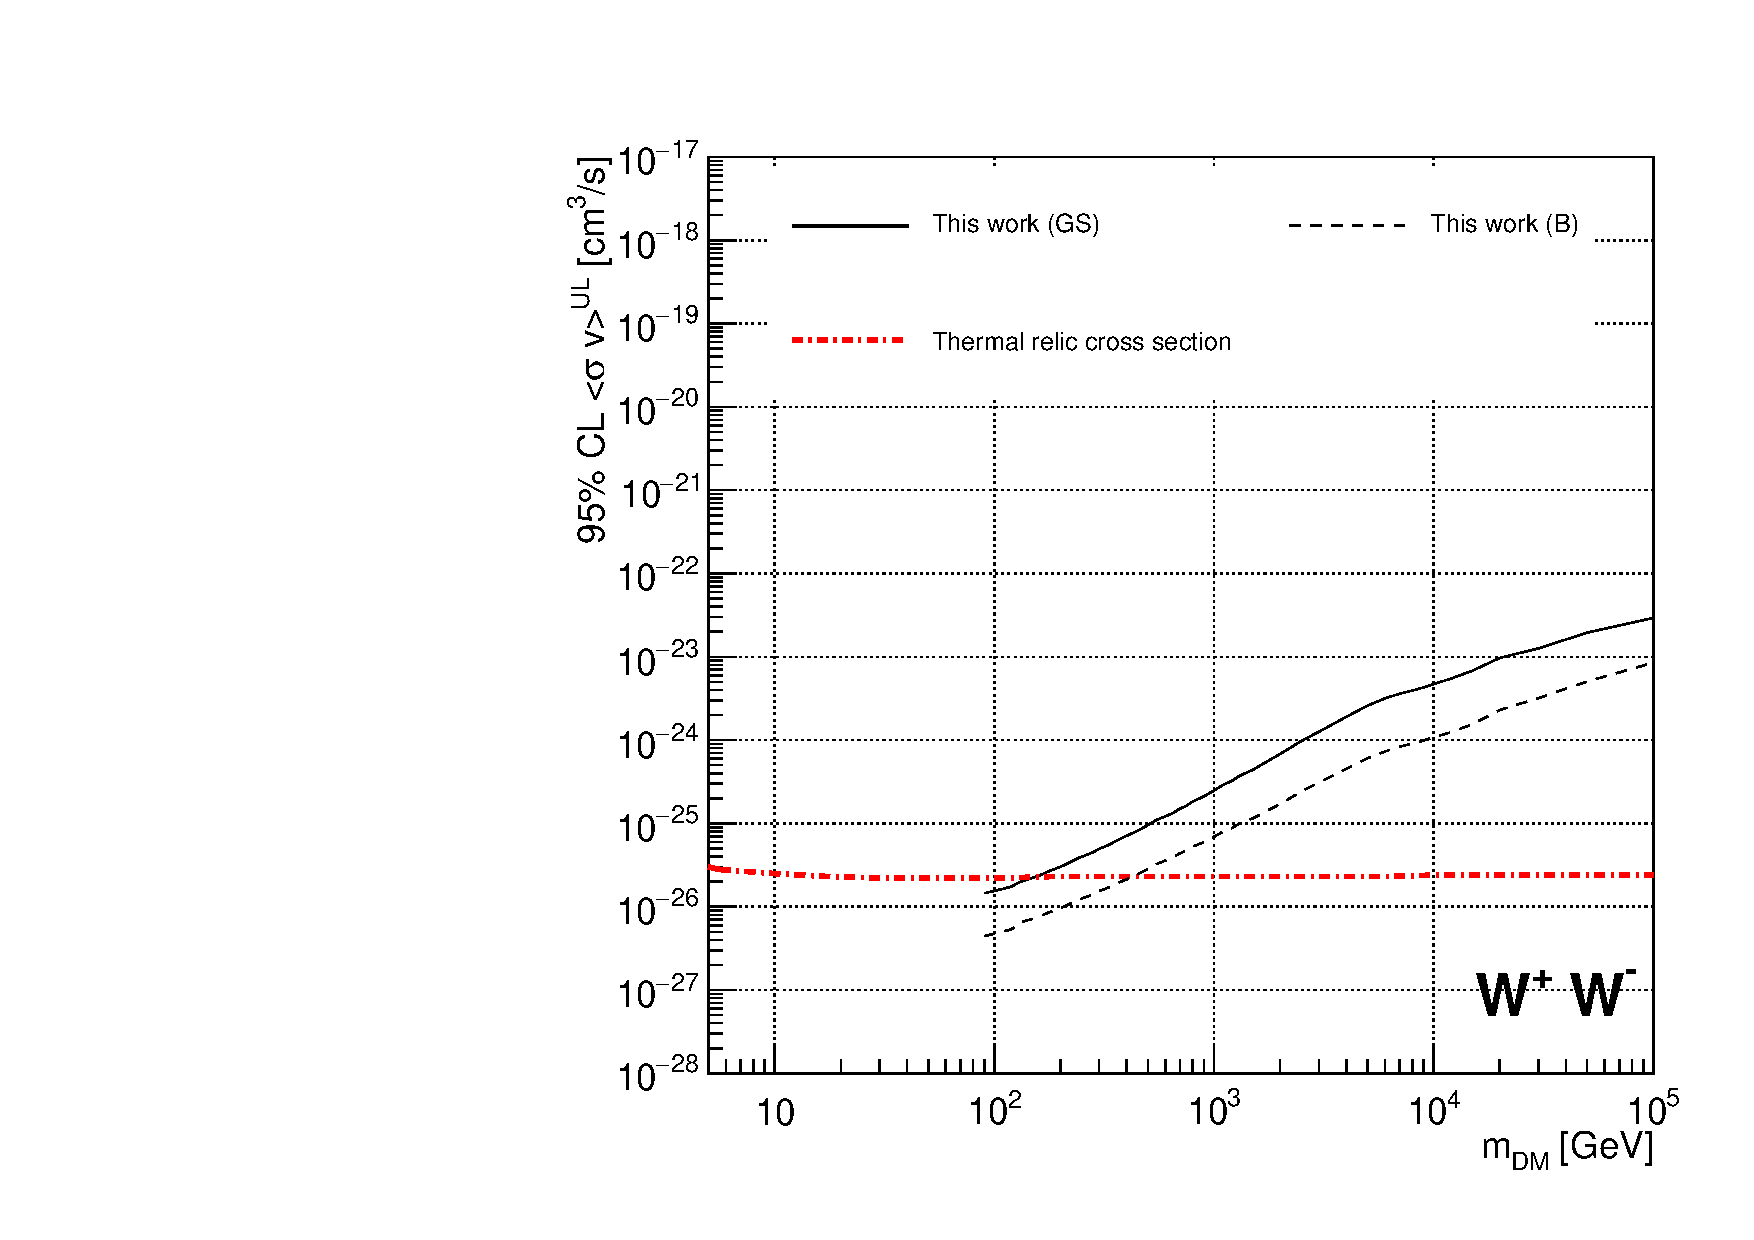
\includegraphics[width=0.3\textwidth]{figures/glory_duck/comparison/GD_limits_WW.pdf} &
    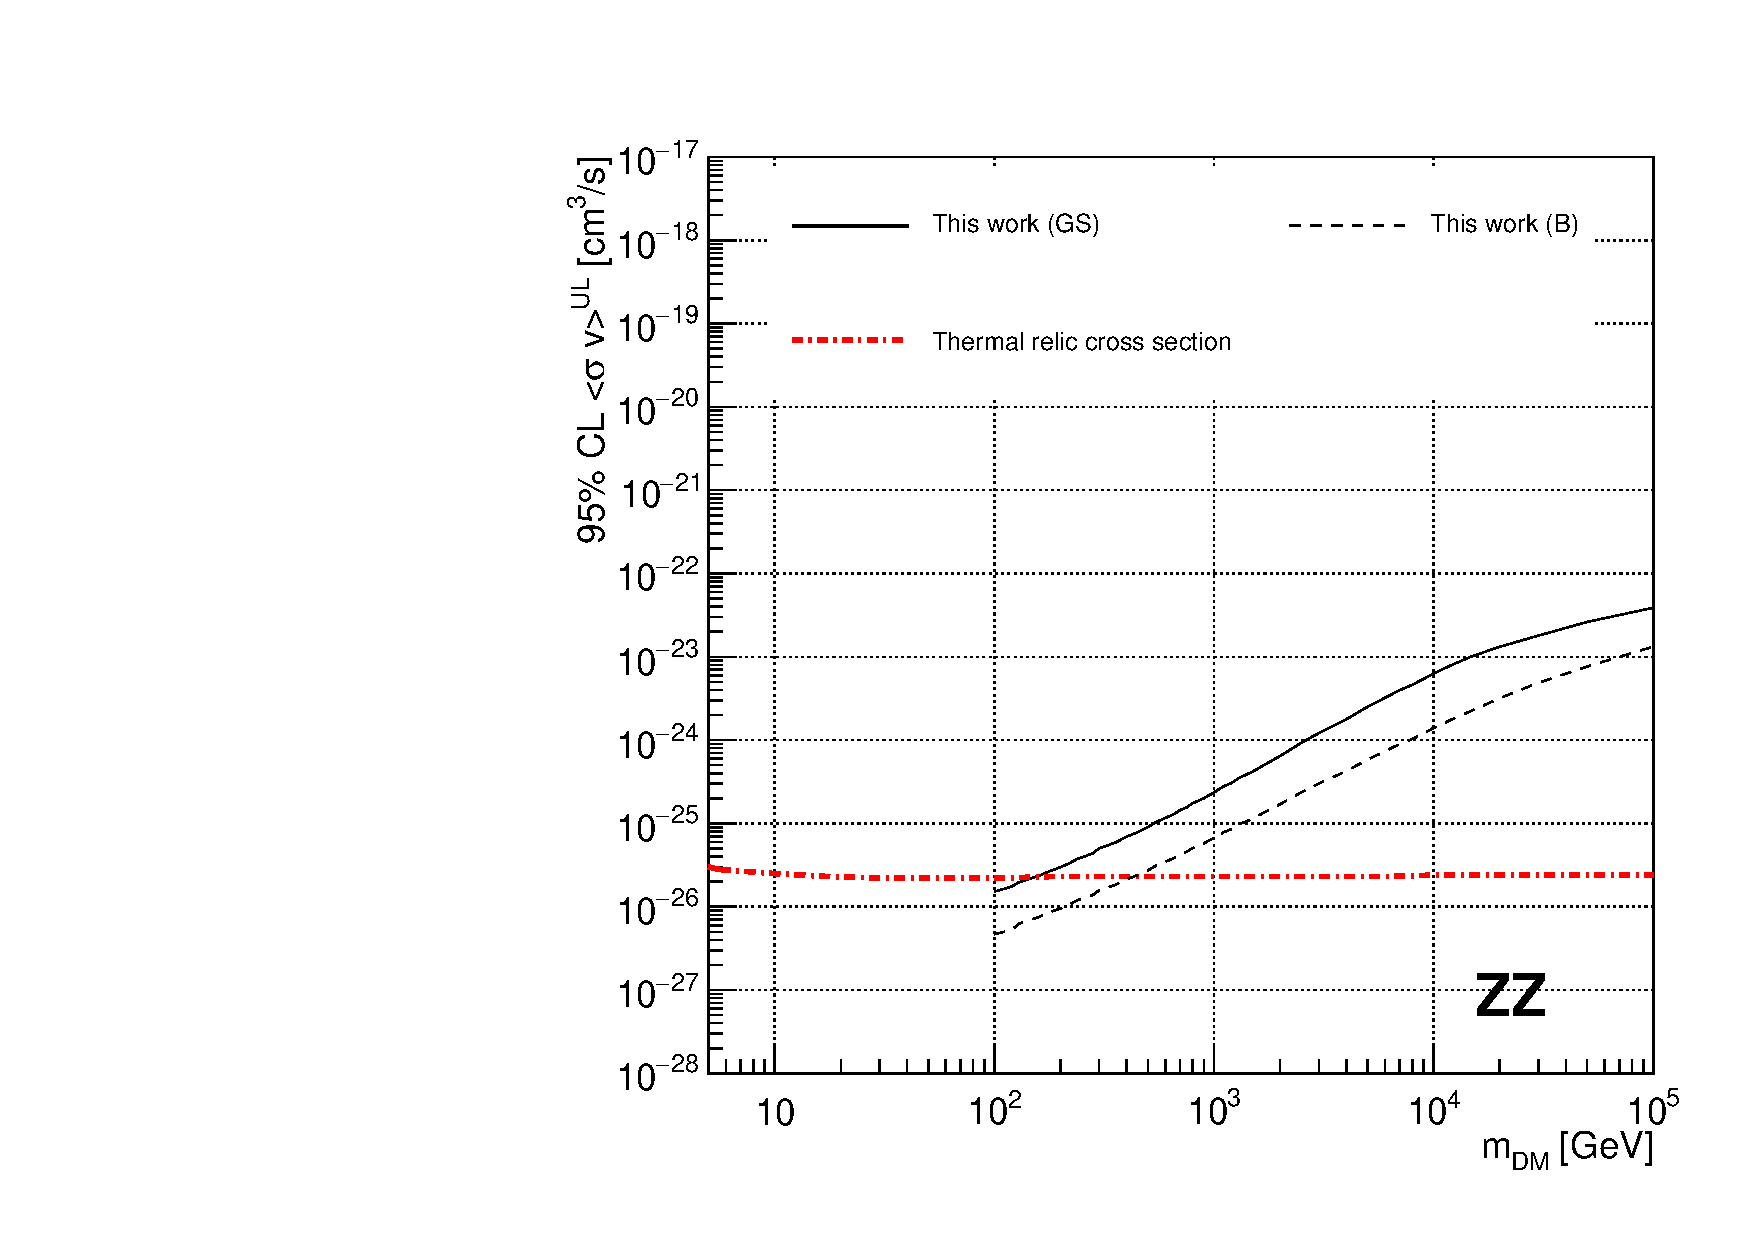
\includegraphics[width=0.3\textwidth]{figures/glory_duck/comparison/GD_limits_ZZ.pdf} &
    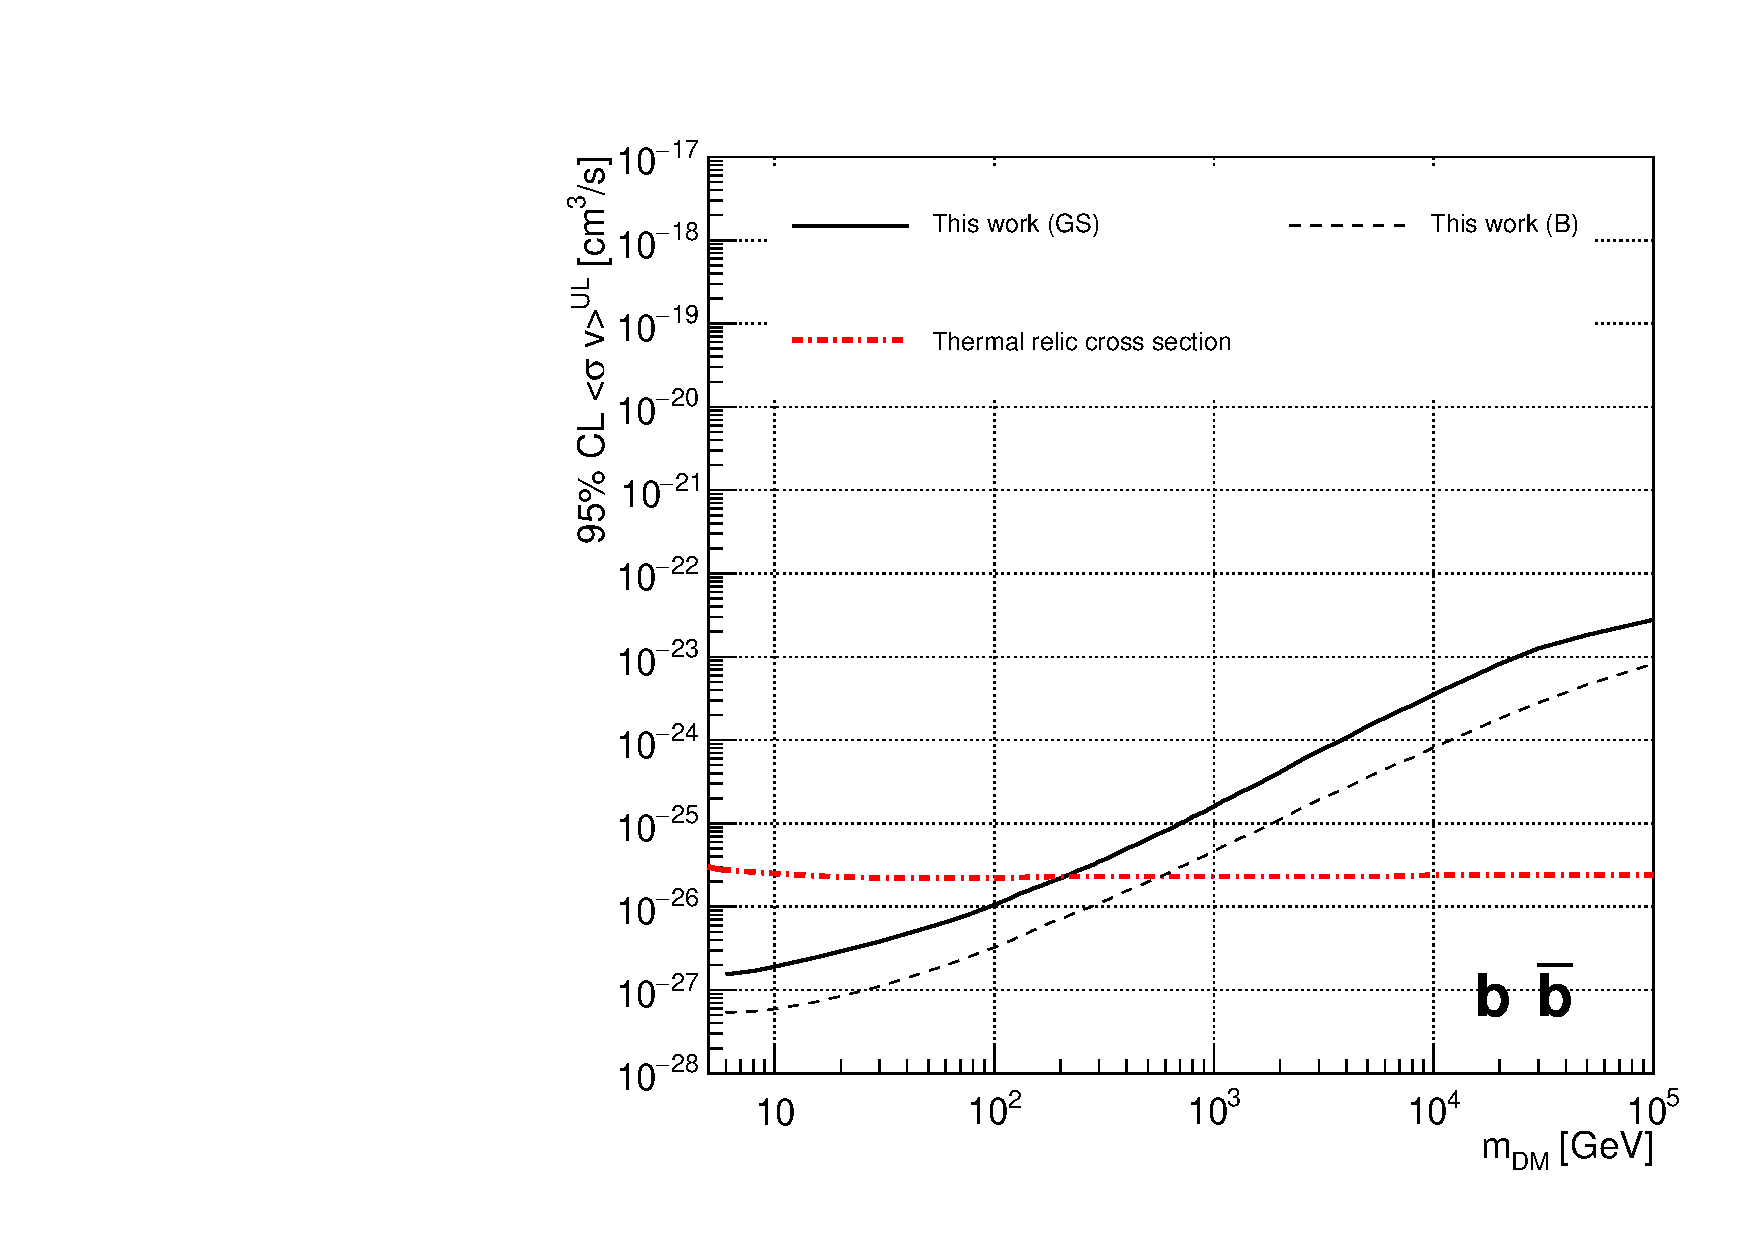
\includegraphics[width=0.3\textwidth]{figures/glory_duck/comparison/GD_limits_bb.pdf} \\
    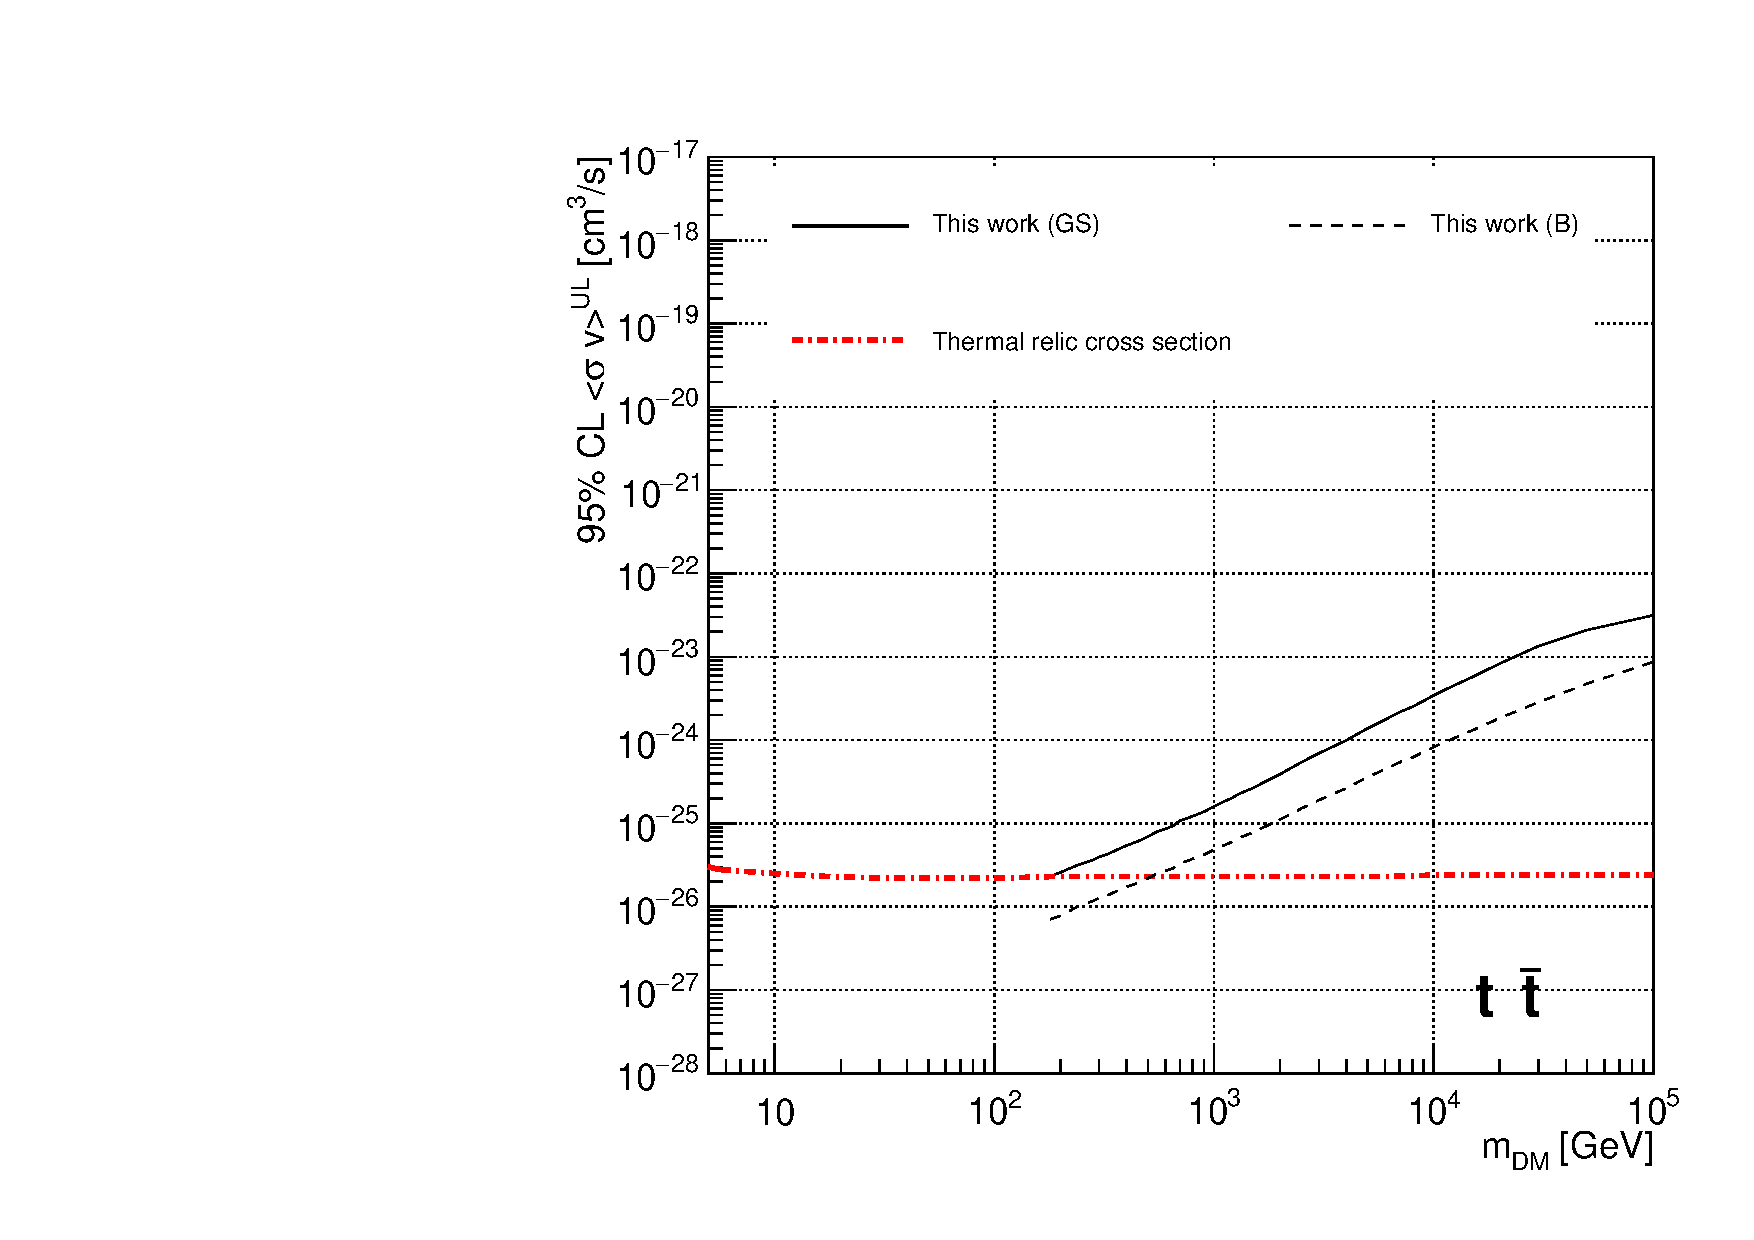
\includegraphics[width=0.3\textwidth]{figures/glory_duck/comparison/GD_limits_tt.pdf} &
    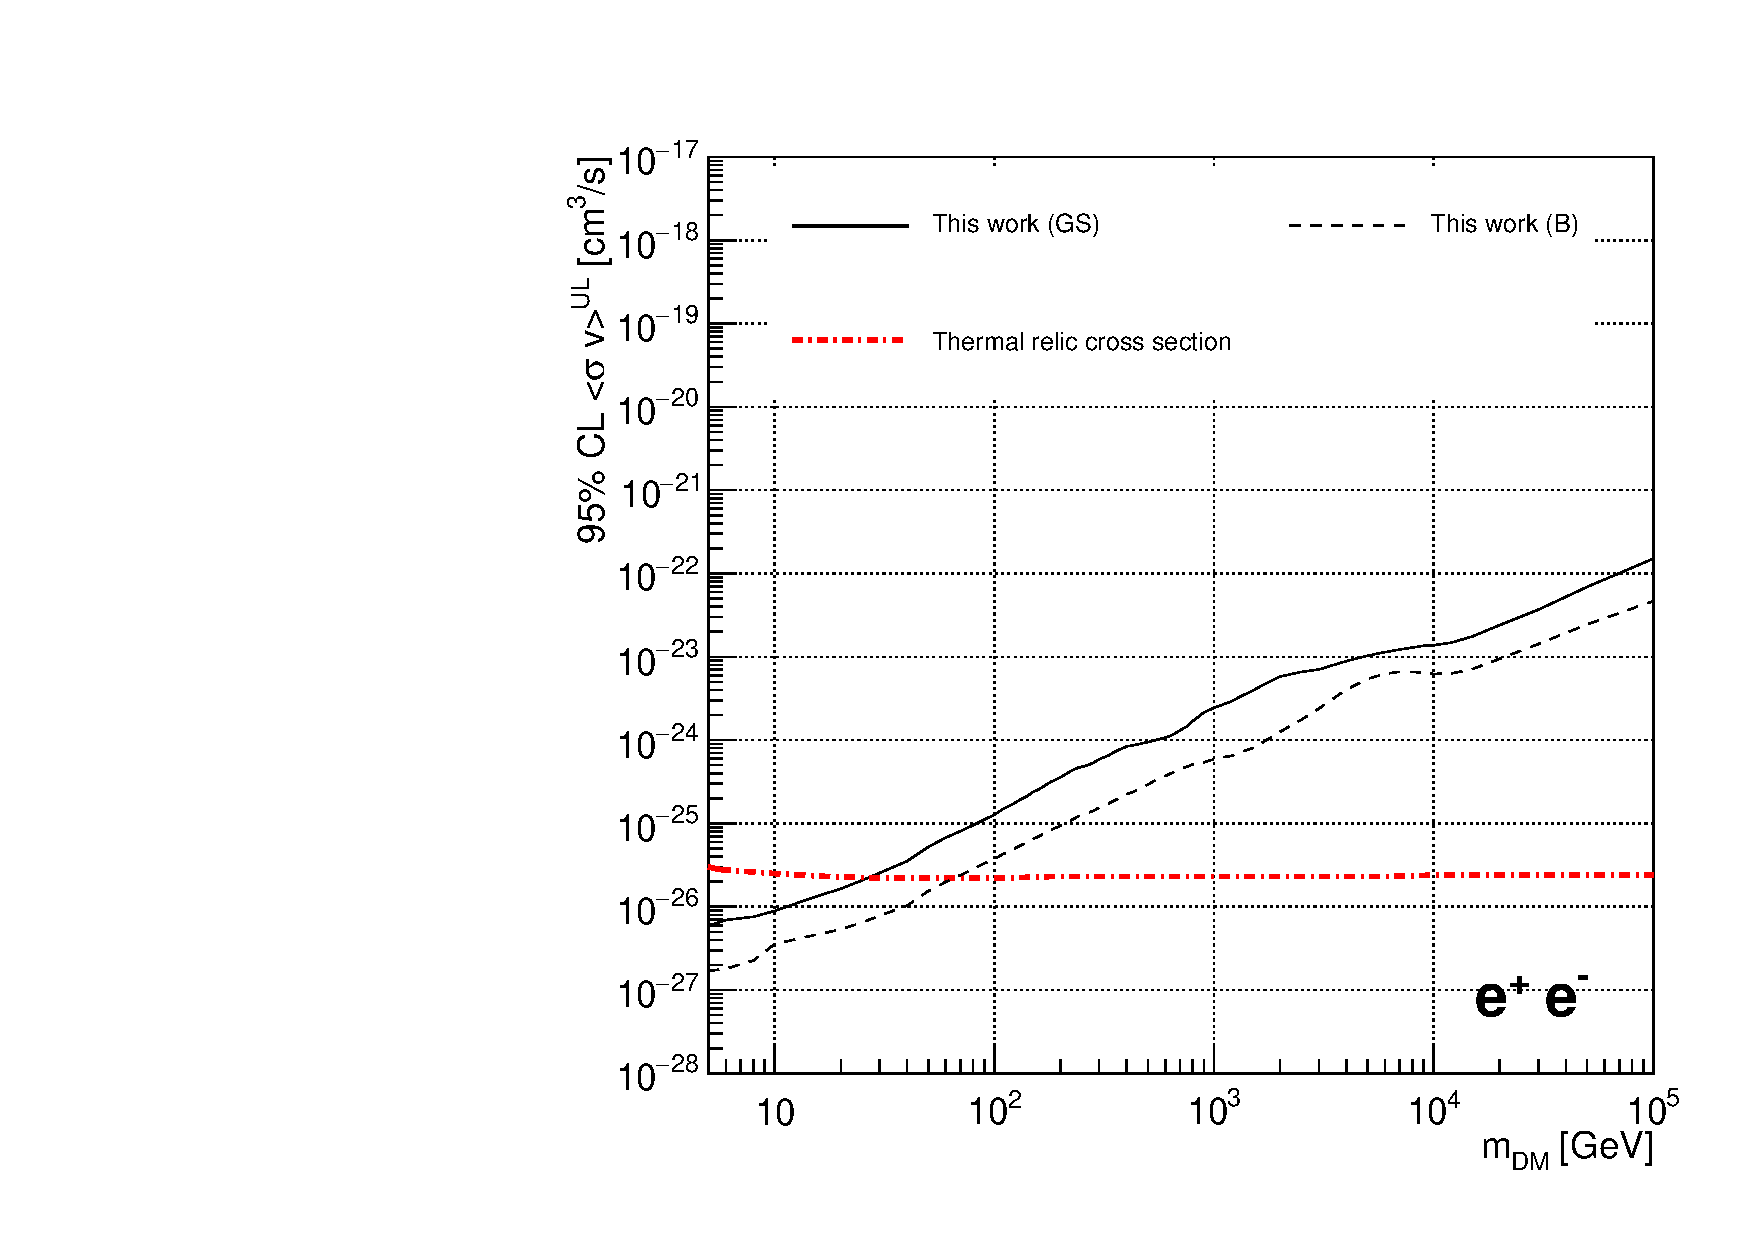
\includegraphics[width=0.3\textwidth]{figures/glory_duck/comparison/GD_limits_ee.pdf} &
    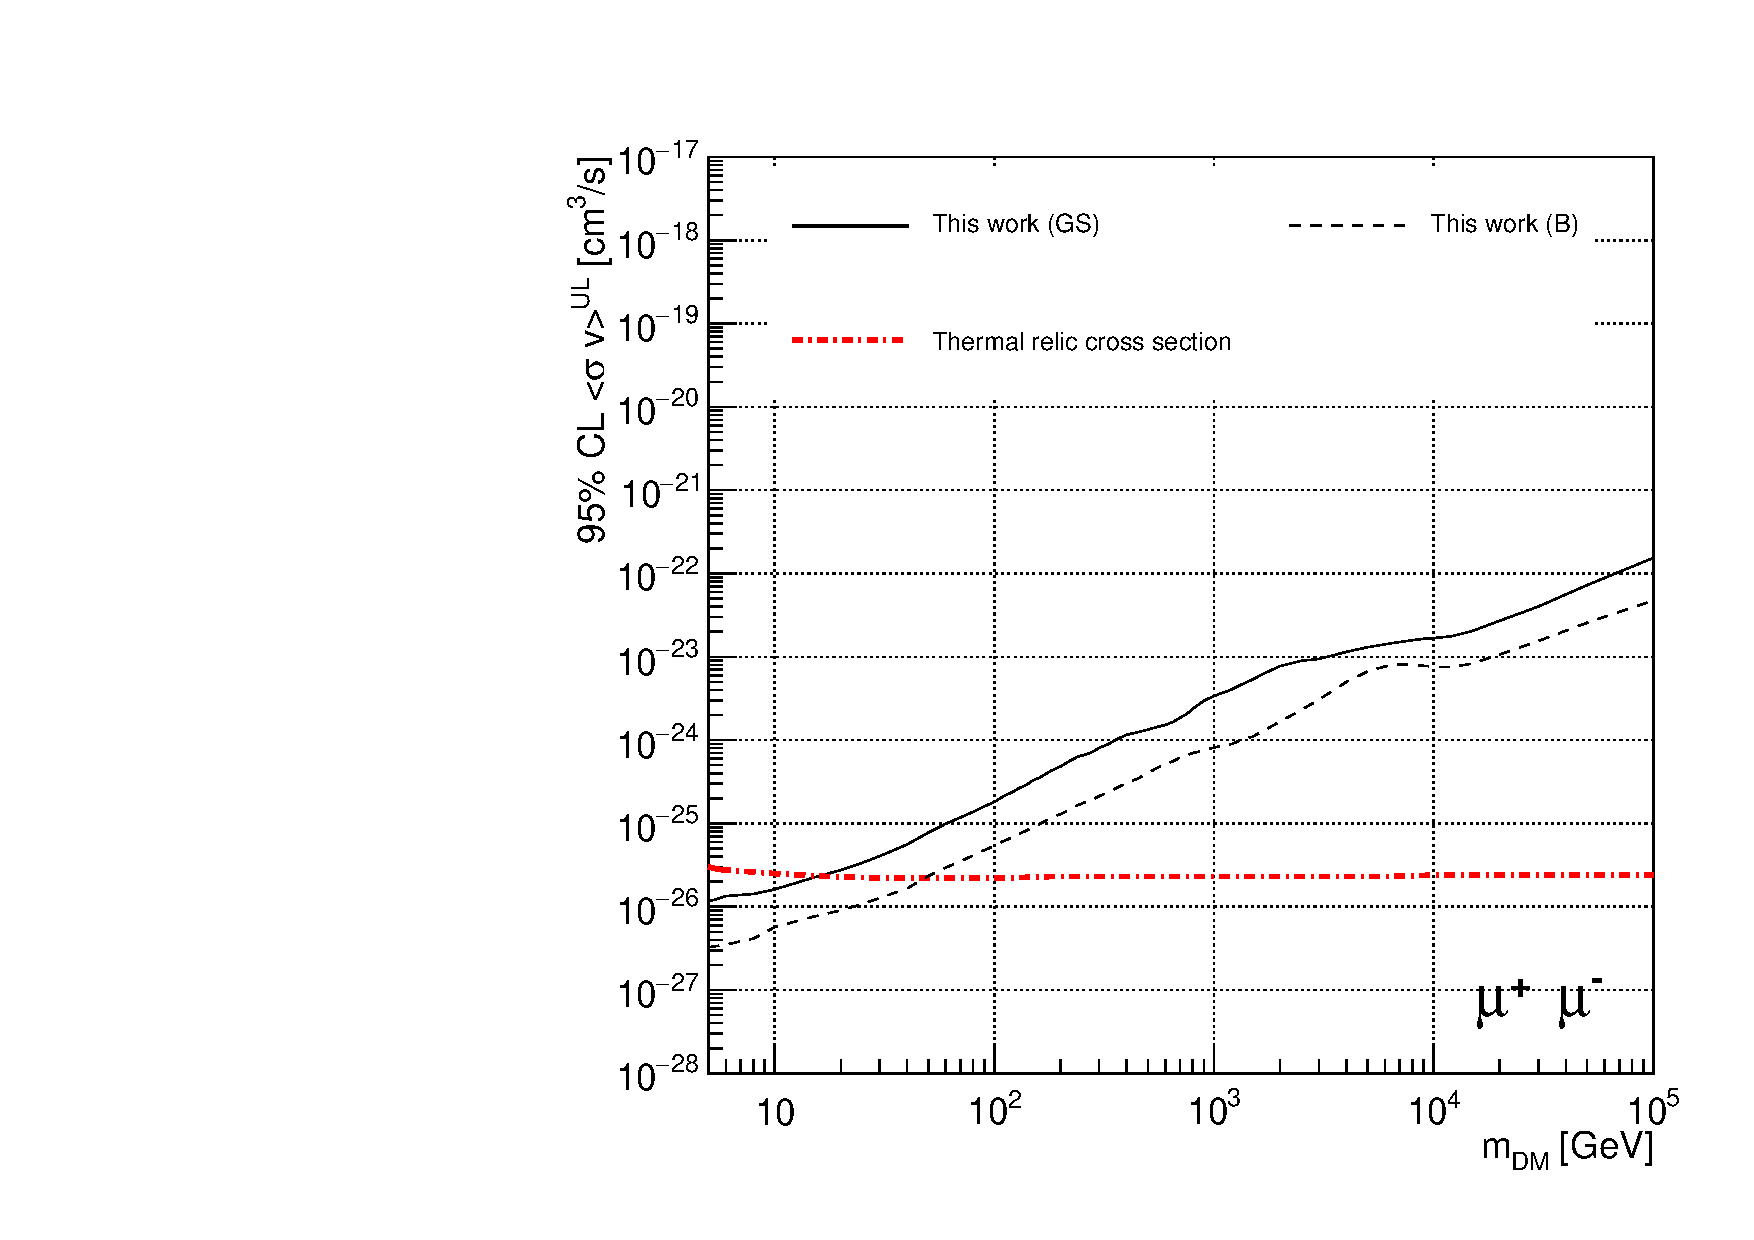
\includegraphics[width=0.3\textwidth]{figures/glory_duck/comparison/GD_limits_mumu.pdf} \\
    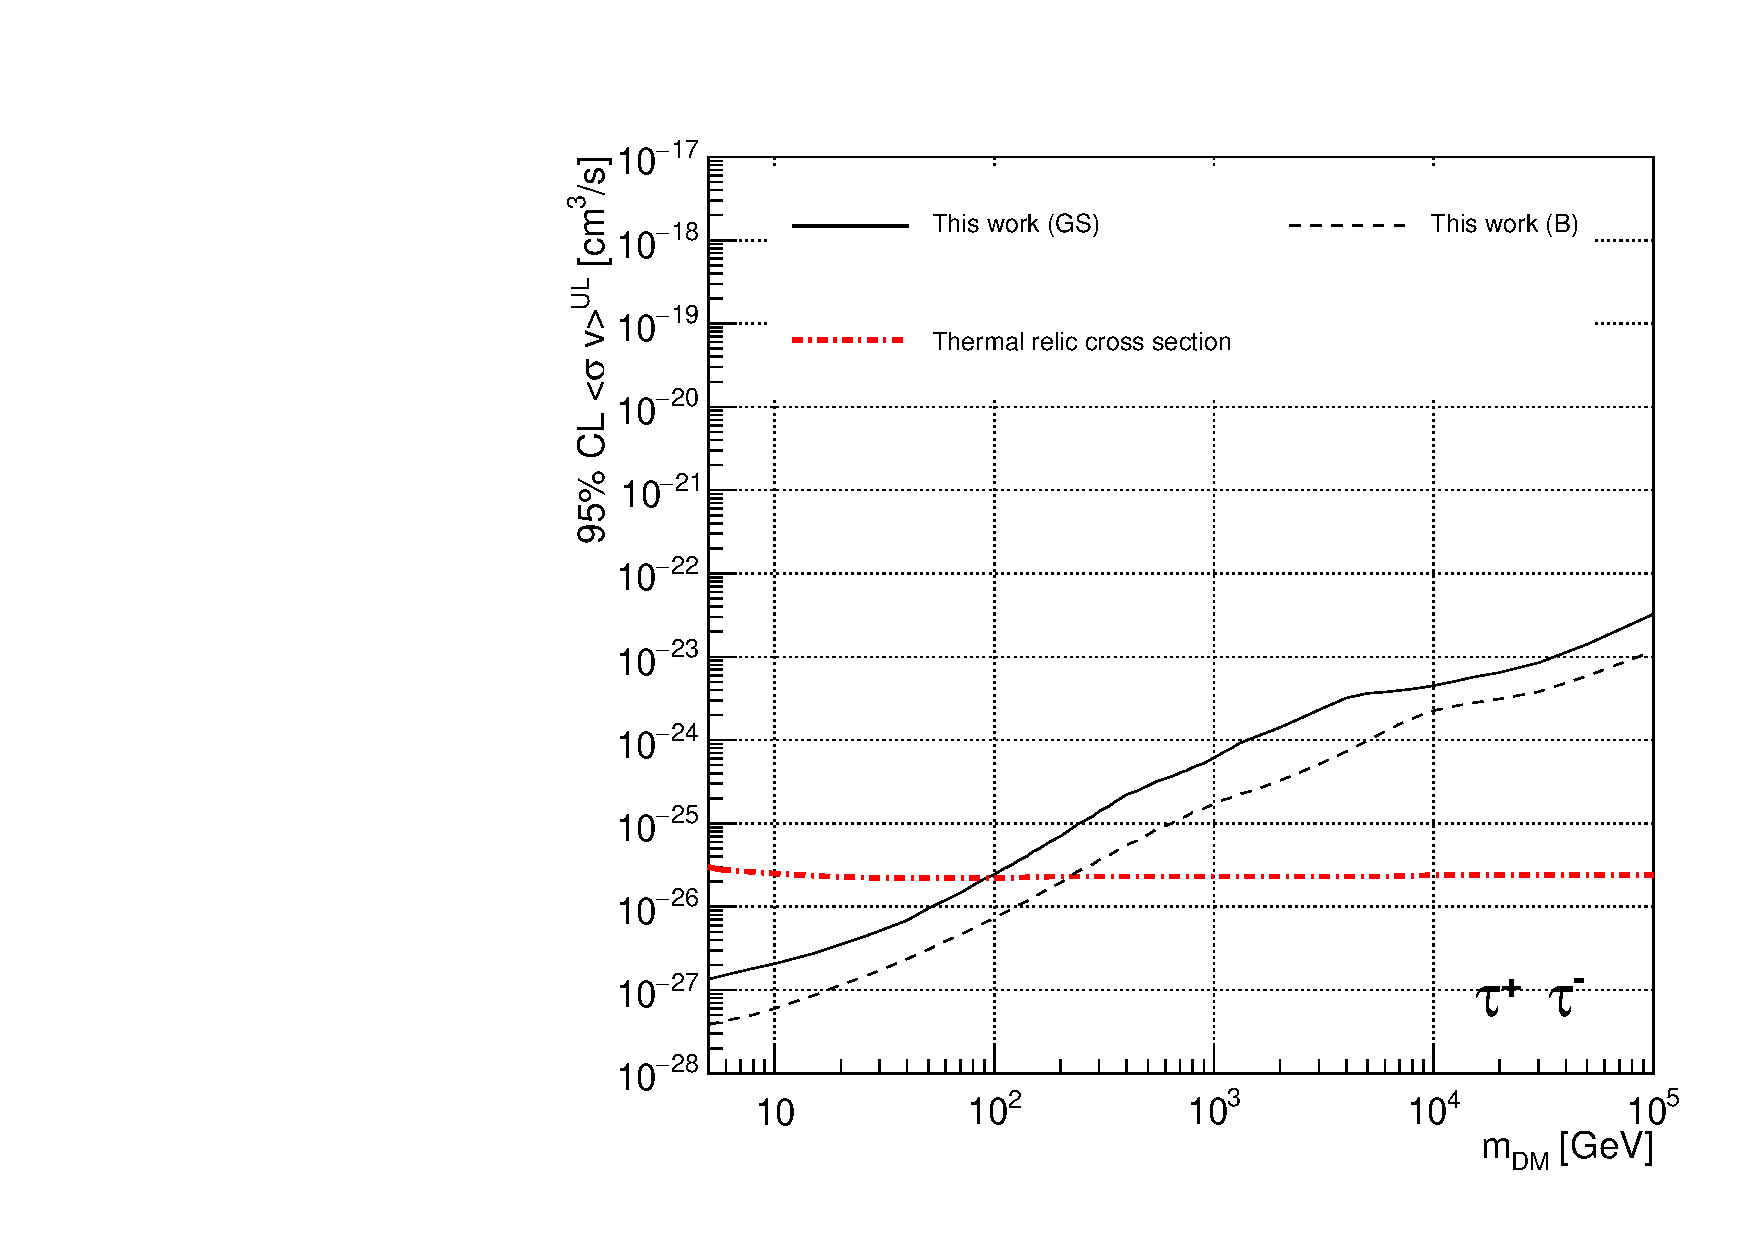
\includegraphics[width=0.3\textwidth]{figures/glory_duck/comparison/GD_limits_tautau.pdf} &
    \end{tabular}
    }
    \caption{Comparisons of the combined limits at 95\% confidence level for each of the eight annihilation channels when using the \J factors from Ref.~\cite{Geringer-Sameth:2014yza} (\GS set in \Cref{tab:gd_J_factor}), plain lines, and the \J factor from Ref.~\cite{Bonnivard:2014kza, Bonnivard:2015xpq} (\B set in \Cref{tab:gd_J_factor}), dashed lines. The cross-section given by the thermal relic is also indicated~\cite{Bertone_2005}.}
\label{fig:limits-comparison}
\end{figure}

%%%%%%%%%%%%%%%%%%%%%%%%%%%%%%%%%%%%%%%%%%%%%%%%%%%%%%%%%%%%%%%%%%%%%%%%%%%%%%%%%%%%%
\section{HAWC Systematics} \label{sec:hawc_systematic}
%%%%%%%%%%%%%%%%%%%%%%%%%%%%%%%%%%%%%%%%%%%%%%%%%%%%%%%%%%%%%%%%%%%%%%%%%%%%%%%%%%%%%

%%%%%%%%%%%%%%%%%%%%%%%%%%%%%%%%%%%%%%%%%%%%%%%%%%%%%%%%%%%%%%%%%%%%
\subsection{Inverse Compton Scattering} \label{sec:gd_ics}
%%%%%%%%%%%%%%%%%%%%%%%%%%%%%%%%%%%%%%%%%%%%%%%%%%%%%%%%%%%%%%%%%%%%
The DM-DM annihilation channels produce many high energy electrons regardless of the primary annihilation channel.
These high energy electrons can produce high energy gamma-rays through Inverse Compton Scattering (ICS).
If this effect is strong, it would change the morphology of the source and increase the total expected gamma-ray counts from any source.
The PPPC \cite{Cirelli_2011} provides tools in Mathematica for calculating the impact of ICS for an arbitrary location in the sky for a specified annihilation channel.
We calculated the change in gamma-ray counts for DM annihilation to primary $e\bar{e}$ for RA and Dec corresponding to Segue1 and Coma Berenices.
These dSphs were chosen because they are the strongest contributors to the limit.
$e\bar{e}$ was selected because it would have the largest number of high energy electrons.
The effect was found to be on the order of $~10^{-7}$ on the gamma-ray spectrum.
As a result, this systematic is not considered in our analysis.

%%%%%%%%%%%%%%%%%%%%%%%%%%%%%%%%%%%%%%%%%%%%%%%%%%%%%%%%%%%%%%%%%%%%
\subsection{Point Source Versus Extended Source Limits}\label{sec:gd_ext_limitvs_ptsrc}
%%%%%%%%%%%%%%%%%%%%%%%%%%%%%%%%%%%%%%%%%%%%%%%%%%%%%%%%%%%%%%%%%%%%

The previous DM search toward dSph approximated the dSphs as point sources \cite{Albert_2018}.
In this analysis, the dSphs are implemented as extended with J-factor distributions following those produced by \cite{Geringer-Sameth:2014yza}.
The resolution of the cited map is much finer than HAWC's angular resolution.
The vast majority of the J-factor distribution is represented on the central HAWC pixel of the dSph spatial map.
However, the neighboring 8 pixels are not negligible and contribute to our limit.

\begin{figure}[ht]
\centering{
    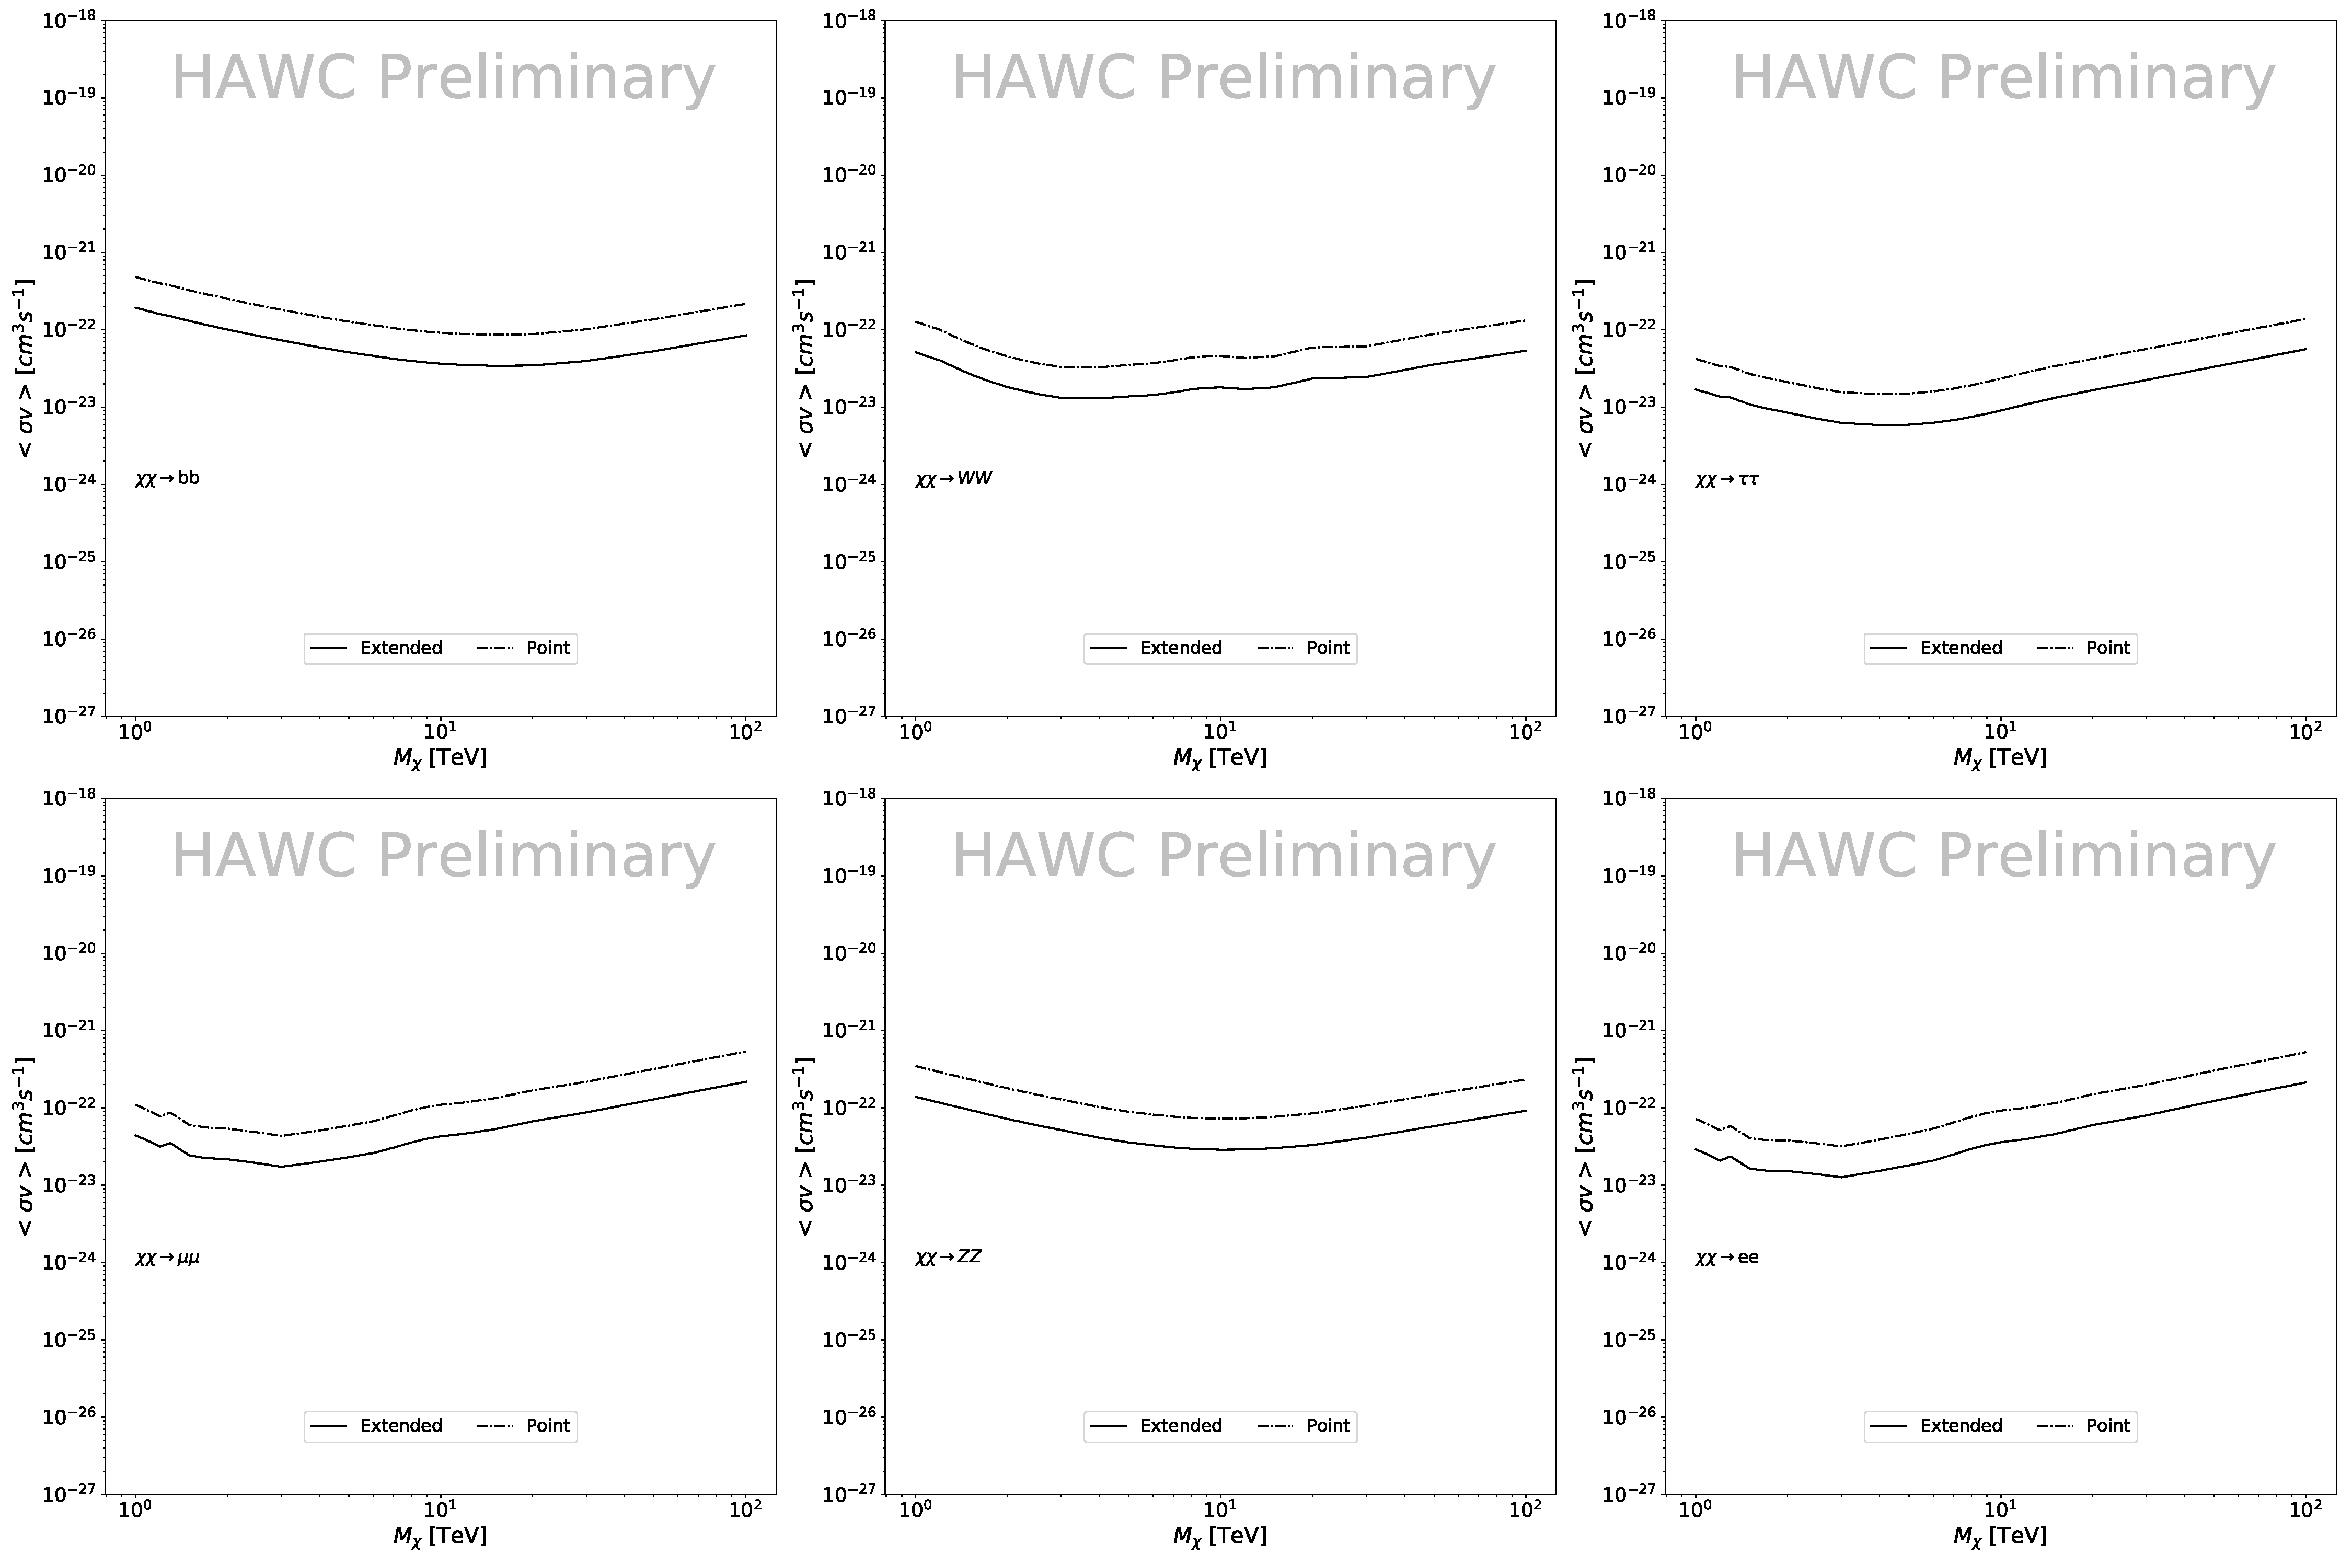
\includegraphics[scale=0.19]{figures/glory_duck/hawc/95Lim_Segue1_ExtVsPt.pdf}}
    \caption{Comparisons of the combined limits at 95\% confidence level for a point source analysis and extended source using ~\cite{Geringer-Sameth:2014yza} \GS J-factor distributions and PPPC \cite{Cirelli_2011} annihilation spectra. Shown are the limits for Segue1 which will have the most significant impact on the combined limit. 6 of the 7 DM annihilation channels are shown. Solid lines are extended source studies. Dashed lines are point source studies. Overall, the extended source analysis improves the limit by a factor of 2.}
\label{fig:Seg1point_versus_extended}
\end{figure}

\begin{figure}[h]
\centering{
    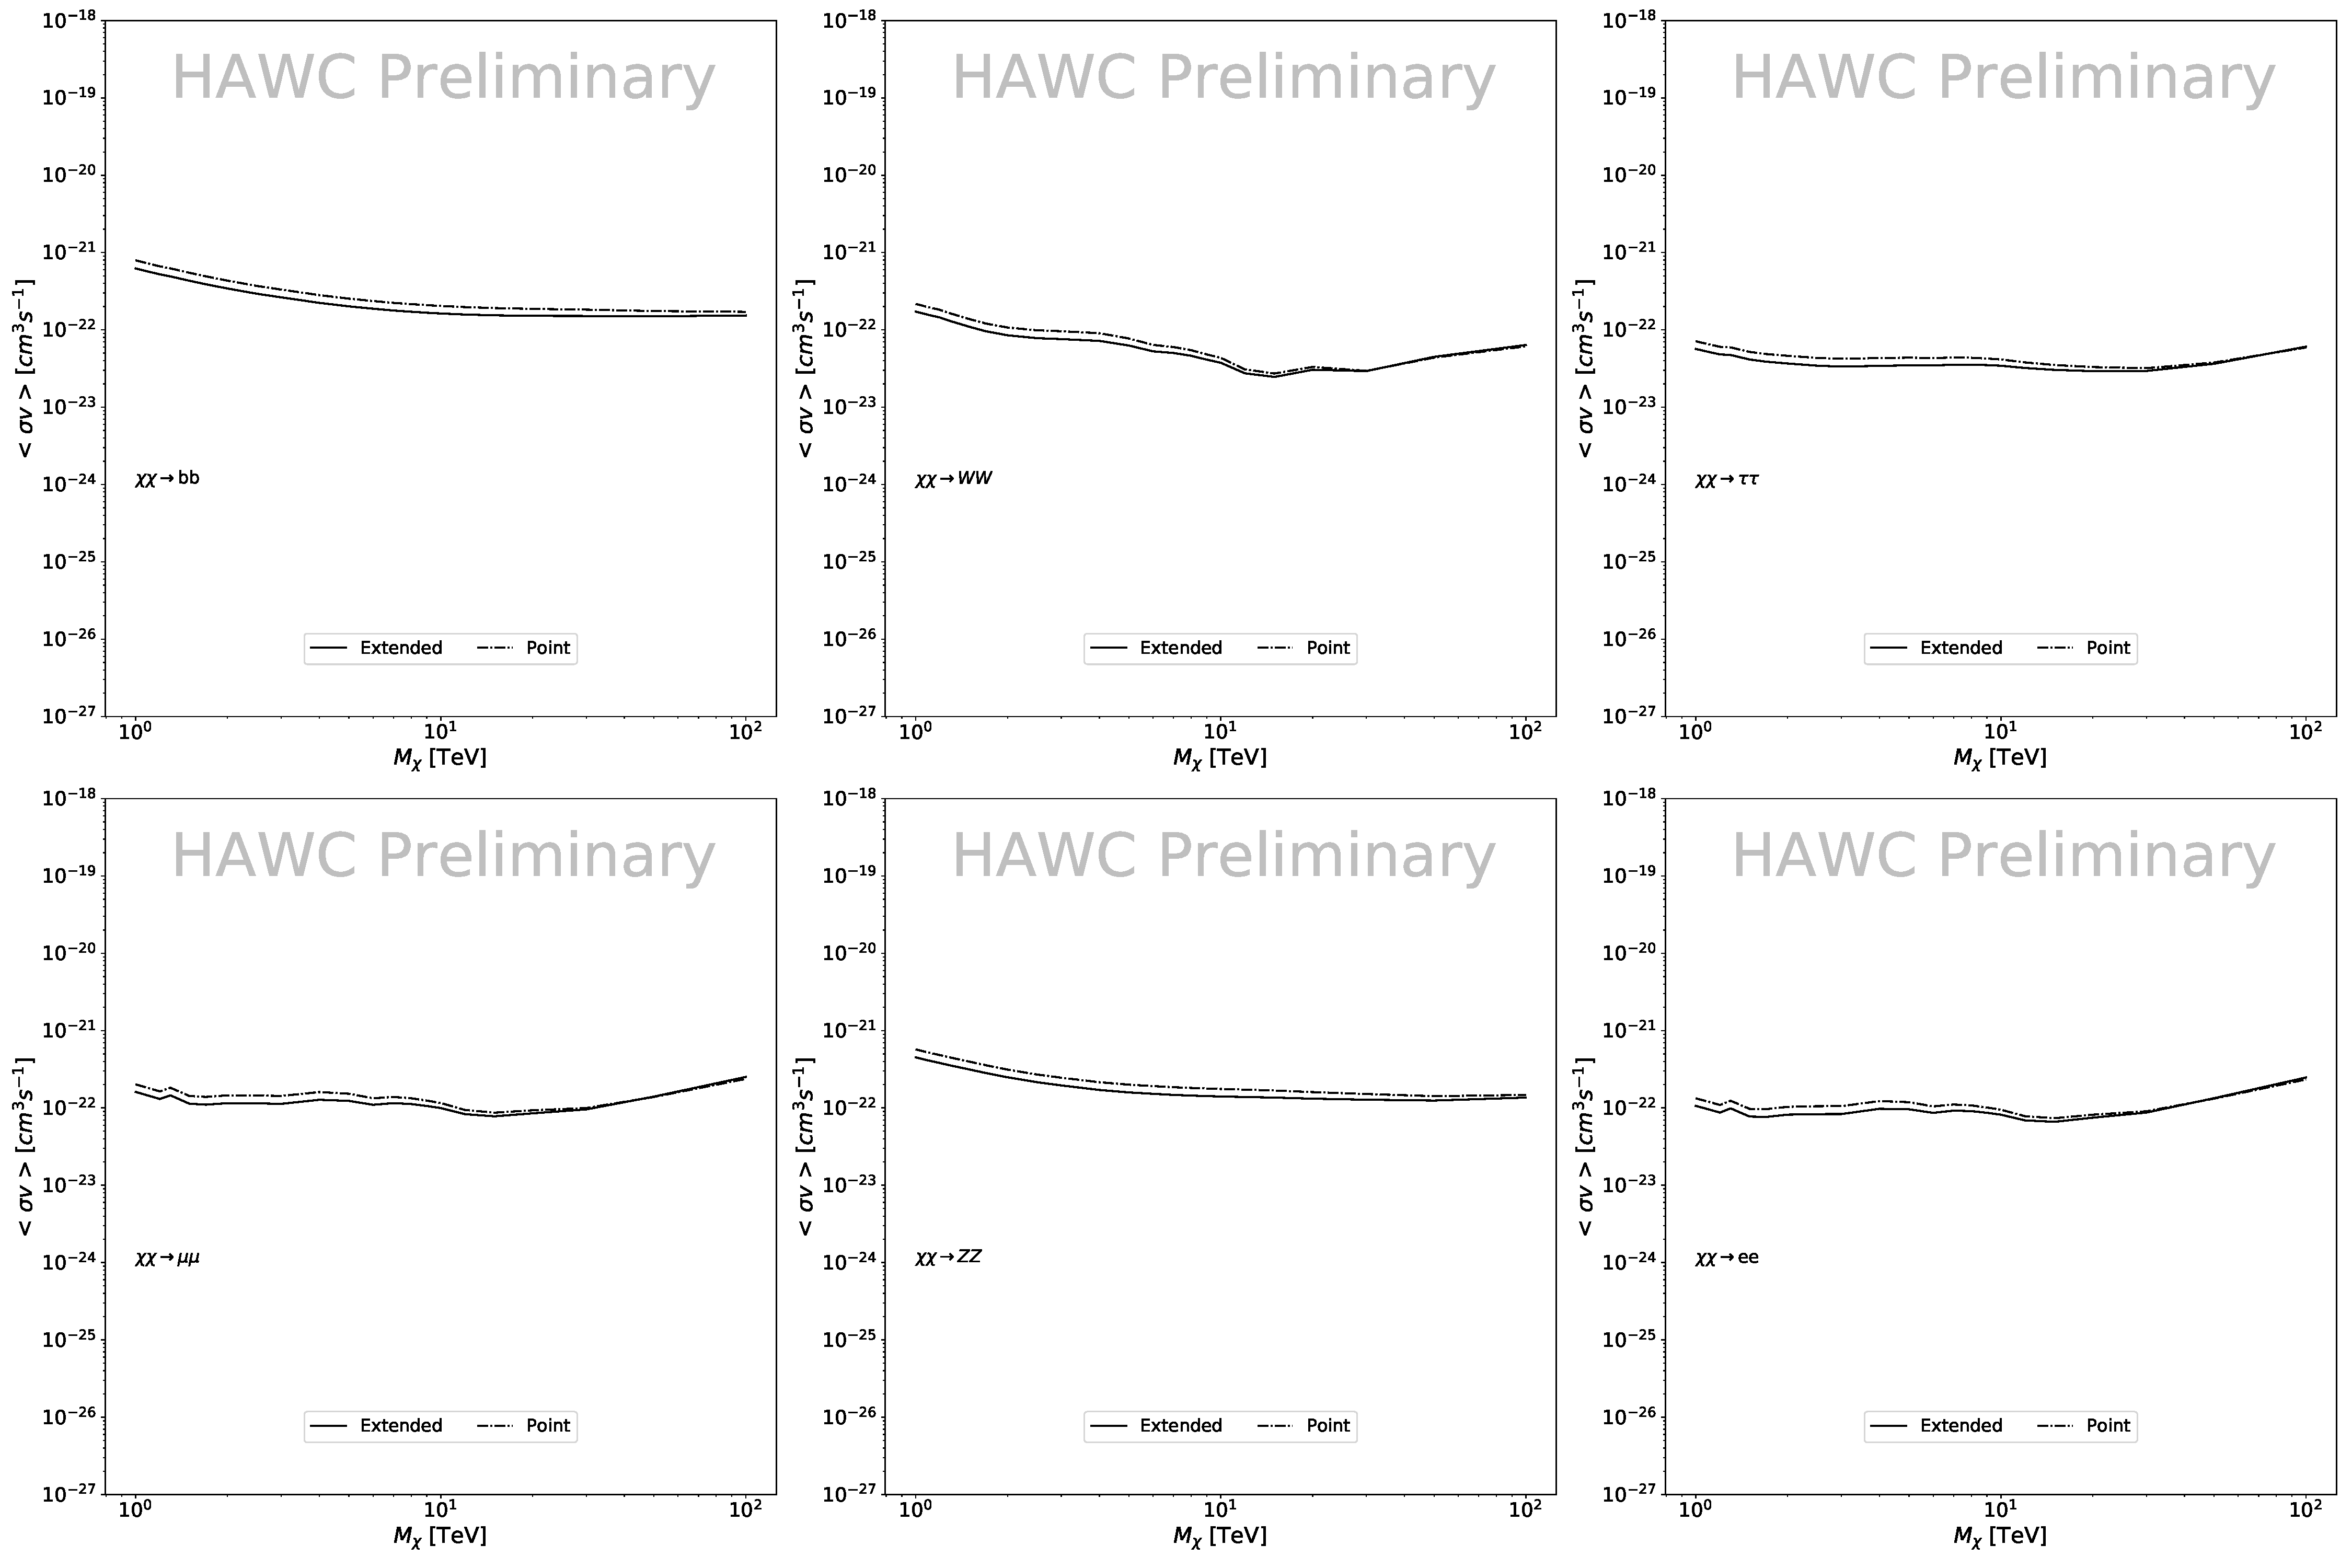
\includegraphics[scale=0.19]{figures/glory_duck/hawc/95Lim_ComaBerenices_ExtVsPt.pdf}}
    \caption{Same as \cref{fig:Seg1point_versus_extended} on Coma Berenices. This dSph also contributes significantly to the limit. The limits are identical in this case.}
\label{fig:ComaBpoint_versus_extended}
\end{figure}

\Cref{fig:Seg1point_versus_extended} shows a substantial improvement to the limit for Segue1.
\cref{fig:ComaBpoint_versus_extended} however showed identical limits.
These disparities are best explained by the relative difference in their J-Factors.
Both dSphs pass almost overhead the HAWC detector, however Segue1 has the larger J-Factor between the two.
Adjacent pixels to the central pixel will therefor contribute to the limits.
This is the case for other dSph that are closer to the zenith of the HAWC detector.

Comparison plots for all sources and the combined limit can be found in the sandbox for the Glory Duck project.

%%%%%%%%%%%%%%%%%%%%%%%%%%%%%%%%%%%%%%%%%%%%%%%%%%%%%%%%%%%%%%%%%%%%
\subsection{Impact of Pointing Systematic}\label{sec:gd_pointing_sys}
%%%%%%%%%%%%%%%%%%%%%%%%%%%%%%%%%%%%%%%%%%%%%%%%%%%%%%%%%%%%%%%%%%%%

During the analysis it was discovered that directional reconstruction of gamma-rays had a systematic bias at large zenith angles.
Slides describing this systematic can be found \href{https://private.hawc-observatory.org/wiki/images/3/30/HAWCMeetingOct2020-AJS-Pointing.pdf}{here}.
Shown on the presentation is dependence on the pointing systematic on declination.
New spatial profiles were generated for every dSph and limits were computed for the adjusted declination.

\Cref{fig:pointing_systematic} demonstrates the impact of this systematic for all DM annihilation channels studied by HAWC. The impact is a tiny improvement, yet mostly identical, to the combined limits.

\begin{figure}[h]
\centering{
    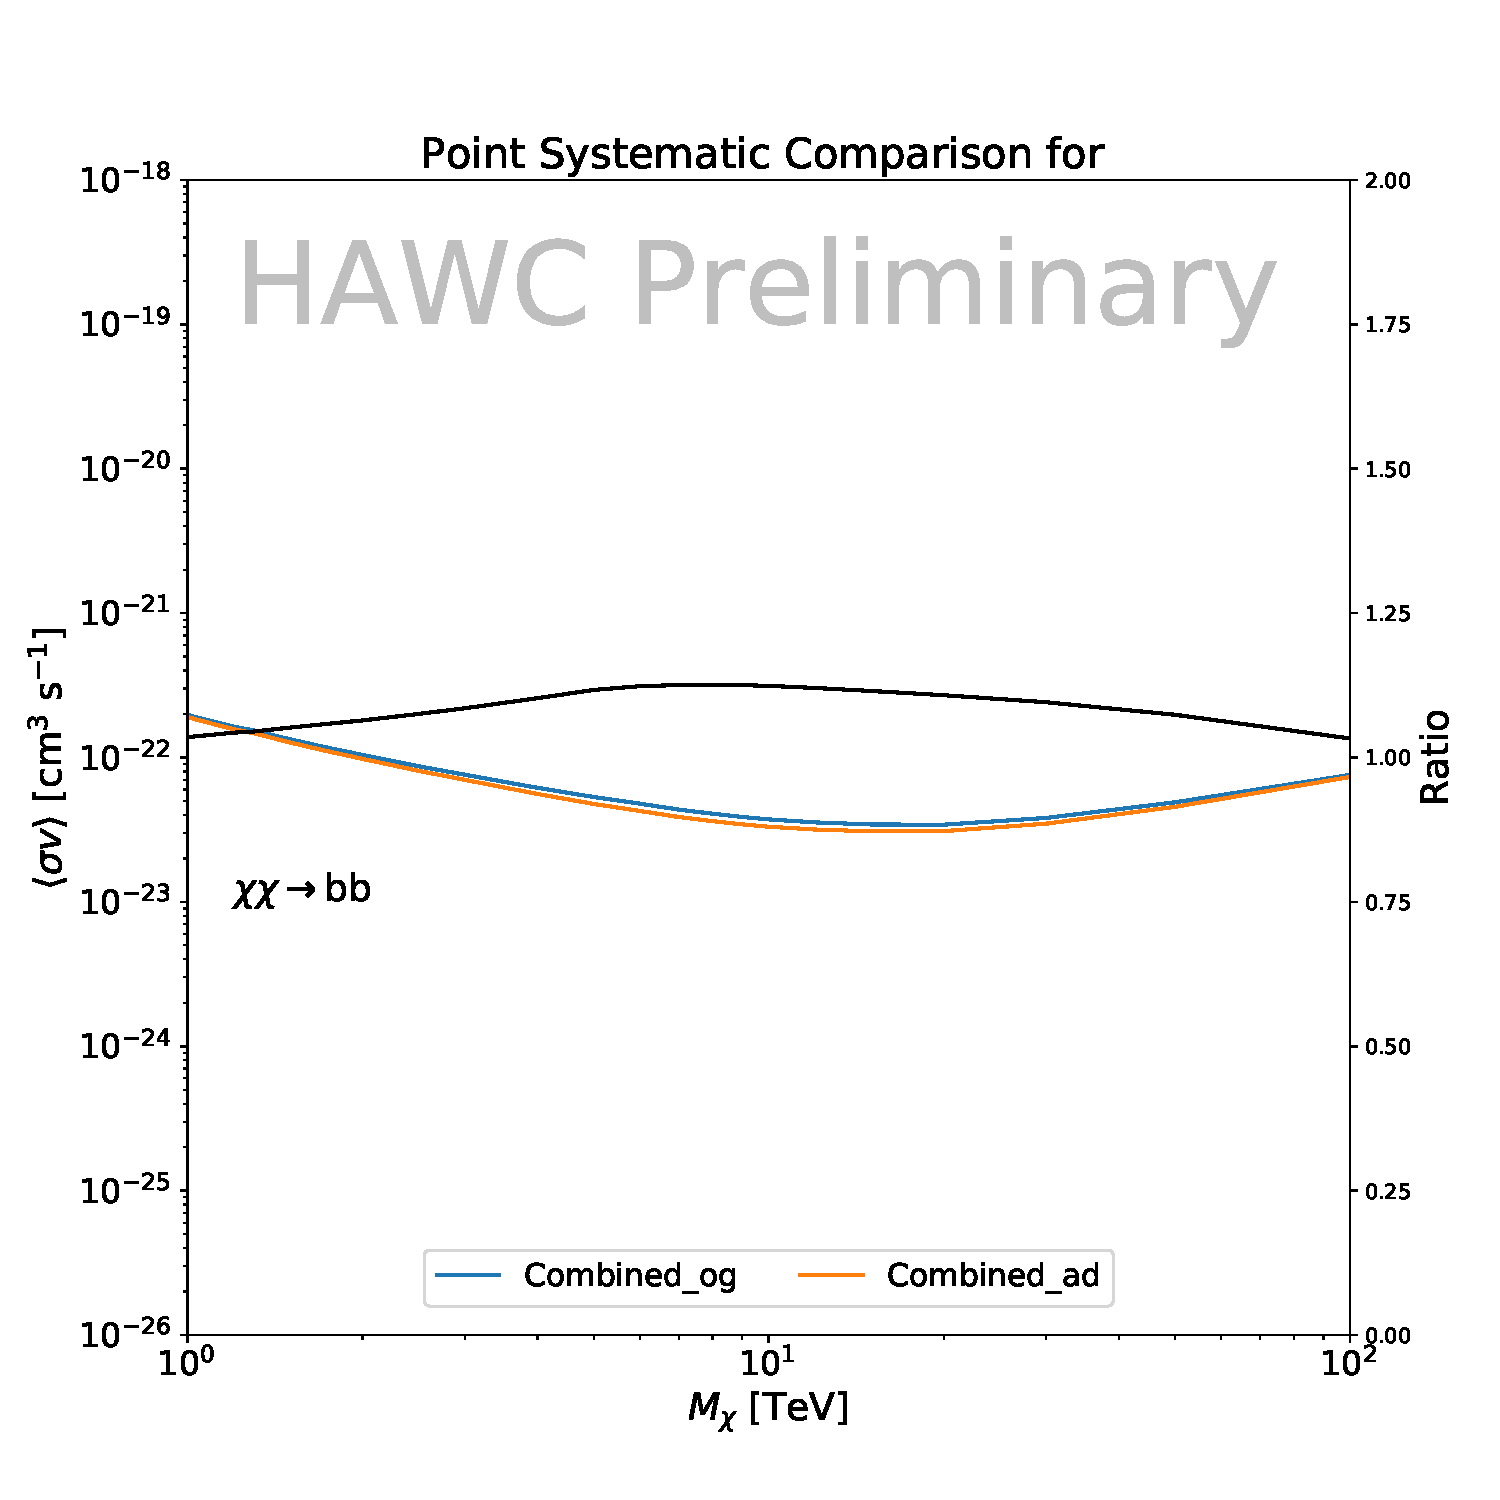
\includegraphics[scale=0.21]{figures/glory_duck/hawc/PointingSystematic_GD_Combined_bb.pdf}
    \includegraphics[scale=0.21]{figures/glory_duck/hawc/PointingSystematic_GD_Combined_ee.pdf}
    \includegraphics[scale=0.21]{figures/glory_duck/hawc/PointingSystematic_GD_Combined_mumu.pdf}
    \includegraphics[scale=0.21]{figures/glory_duck/hawc/PointingSystematic_GD_Combined_tautau.pdf}
    \includegraphics[scale=0.21]{figures/glory_duck/hawc/PointingSystematic_GD_Combined_tt.pdf}
    \includegraphics[scale=0.21]{figures/glory_duck/hawc/PointingSystematic_GD_Combined_ww.pdf}
    \includegraphics[scale=0.21]{figures/glory_duck/hawc/PointingSystematic_GD_Combined_zz.pdf}
    \caption{Comparison of combined limits when correcting for HAWC's pointing systematic. All DM annihilation channels are shown. The solid black line is the ratio between published limit to the declination corrected limit. The blue solid line or "Combined\_og" represented the limits computed for Glory Duck. The solid orange line or "Combined\_ad" represented the limits computed after correcting for the pointing systematic.}
}
\label{fig:pointing_systematic}
\end{figure}

%%%%%%%%%%%%%%%%%%%%%%%%%%%%%%%%%%%%%%%%%%%%%%%%%%%%%%%%%
\section{\J-factor distributions}\label{sec:gd_jfactor_systematic}
%%%%%%%%%%%%%%%%%%%%%%%%%%%%%%%%%%%%%%%%%%%%%%%%%%%%%%%%%

%%%%%%%%%%%%%%%%%%%%%%%%%%%%%%%%%%%%%%%%%%%%%%%%%%%%%%%%%
\subsection{Numerical integration of \GS maps}\label{sec:gd_jfacintegration}
%%%%%%%%%%%%%%%%%%%%%%%%%%%%%%%%%%%%%%%%%%%%%%%%%%%%%%%%%

It was discovered well after the HAWC analysis was completed that the published tables from \GS \cite{Geringer_Sameth_2015} quoted median \J-factors were computed in a non-trivial manner.
The assumption myself and collaborators had been that the published tables represented the \J-factor as a function of $\theta$ for the best global fit model on a per-source basis.
However, this is not the case.
Instead, what is published are the best fit model for each dwarf that only considers stars up to the angular separation $\theta$.
Therefore, the model is changing for each value of $\theta$ for each dwarf.
Yet, the introduced features from unique models at each $\theta$ are much smaller than the angular resolution of HAWC.
It is not expected for these effects to impact the limits and TS greatly as a result.

Median \J-factor model profiles were provided by the authors.
New maps were generated and analyzed for Segue1 and Coma Berenices.
\Cref{fig:gd_djmap_diff} shows the differential between maps generated with the method from \Cref{sec:gd_jfacintegration} and from the authors of \cite{Geringer_Sameth_2015}.
These maps were reanalyzed for all SM DM annihilation channels.
Upper limits for these channels are shown in \Cref{fig:gd_jfacmodel_systematic}

From \Cref{fig:gd_jfacmodel_systematic}, we can see that the impact of these model difference was no substantial.
The observed impact was a fractional effect which is much smaller than the impact from selecting another DM spatial distribution model as was shown in \Cref{fig:limits-comparison}.

\begin{figure}
    \centering{
    \includegraphics[scale=0.5]{figures/glory_duck/hawc/Segue1_diff.png}
    \includegraphics[scale=0.5]{figures/glory_duck/hawc/ComaB_diff.png}
    }
    \caption{Differential map of $d\J/\Omega$ from model built in \Cref{sec:gd_jfacintegration} and profiles provided directly from authors. (Top) Differential from Segue1. (bottom) Differential from Coma Berenices. Note that their scales are not the same. Segue1 shows the deepest discrepancies which is congruent with its large uncertainties. Both models show anuli where unique models become apparent.}\label{fig:gd_djmap_diff}
\end{figure}

\begin{figure}
    \centering{
        \includegraphics[scale=0.38]{figures/glory_duck/hawc/JFacModel_Systematic_GD_ComaBerenices_bb.pdf}
        \includegraphics[scale=0.38]{figures/glory_duck/hawc/JFacModel_Systematic_GD_Segue1_bb.pdf}
    }
    \caption{HAWC limits for Coma Berenices (top) and Segue1 (bottom) for two different map sets. Blue lines are limits calculated on maps with poor model representation. Orange lines are limits calculated on spatial profiles provided by the authors of \cite{Geringer_Sameth_2015}. Black line is the ratio of the poor spatial model limits to the corrected spatial models. The left y-axis measures \sv for the blue and orange lines. The right y-axis measures the ratio and is unitless.}\label{fig:gd_jfacmodel_systematic}
\end{figure}

%%%%%%%%%%%%%%%%%%%%%%%%%%%%%%%%%%%%%%%%%%%%%%%%%%%%%%%%%
\subsection{\GS Versus \B spatial models}\label{sec:gd_gsVb}
%%%%%%%%%%%%%%%%%%%%%%%%%%%%%%%%%%%%%%%%%%%%%%%%%%%%%%%%%

We show in this appendix a comparison between the \J-factors computed by Geringer-Sameth \emph{et al.}~\cite{Geringer-Sameth:2014yza} (the \GS set) and the ones computed by Bonnivard \emph{et al.}~\cite{Bonnivard:2014kza, Bonnivard:2015xpq} (the \B set).
%The differences in computation between both sets are detailed in \cref{sec:DM}.
%
The \GS \J-factors are computed through a Jeans analysis of the kinematic stellar data of the  selected dSphs, assuming a dynamic equilibrium and a spherical symmetry for the dSphs.
They adopted the generalized DM density distribution, known as Zhao-Hernquist, introduced by~\cite{Zhao:1995cp}, carrying three additional index parameters to describe the inner and outer slopes, and the break of the density profile.
Such a profile parametrization allows the reduction of the theoretical bias from the choice of a specific radial dependency on the kinematic data.
In other words, the increase of free parameters with the use of the  Zhao-Hernquist profile allows a better description of the mass density distribution of dark matter.

In addition, a constant velocity anisotropy profile and a Plummer light profile \cite{10.1093/mnras/71.5.460} for the stellar distribution were assumed.
The velocity anisotropy profile depends on the radial and tangential velocity dispersion.
However, its determination remains challenging since only the line-of-sight velocity dispersion can be derived from velocity measurements.
Therefore, the parametrization of the anisotropy profile is obtained from simulated halos (see~\cite{Hunter:2013vua} for more details).
They provide the values of the \J-factors of regions extending to various angular radius up to the outermost member star.

The \B \J-factors were computed through a Jeans analysis taking into account the systematic uncertainties induced by the DM profile parametrization, the radial velocity anisotropy profile, and the triaxiality of the halo of the dwarf galaxies.
They performed a more complete study of the dSph kinematics and dynamics than \GS for the determination of the \J-factor.
Conservative values of the \J-factors where obtained using an Einasto DM density profile~\cite{Dhar_2010}, a realistic anisotropy profile known as the Baes \& Van Hese profile~\cite{Baes:2007tx} which takes into account that the inner regions can be significantly non-isotropic, and a Zhao-Hernquist light profile~\cite{Zhao:1995cp}.

For both sets, \J-factor values are provided for all dSphs as a function of the radius of the integration region~\cite{Geringer-Sameth:2014yza,Bonnivard:2014kza,Bonnivard:2015xpq}.
\Cref{tab:gd_J_factor} shows the heliocentric distance and Galactic coordinates of the twenty dSphs, together with the two sets of \J-factor values integrated up to the outermost observed star for \GS and the tidal radius for \B.
Both \J-factor sets were derived through a Jeans analysis based on the same kinematic data, except for Draco where the measurements of~\cite{2015MNRAS.448.2717W} have been adopted in the computation of the \B value.
The computations for producing the \GS and \B samples differ in the choice of the DM density, velocity anisotropy, and light profiles, for which the set \B takes into account some sources of systematic uncertainties.

\Cref{fig:comparison_J_1} and \Cref{fig:comparison_J_2} show the comparisons for the \J-factor versus the angular radius for each of the 20 dSphs used in this study.
The uncertainties provided by the authors are also indicated in the figures.
For the \GS set, the computation stops at the angular radius corresponding to the outermost observed star, while for the \B set, the computation stops at the angular radius corresponding to the tidal radius.

\begin{figure}[ht]
\centering{
    \includegraphics[scale=0.32]{figures/glory_duck/appendix/BootesI.pdf}
    \includegraphics[scale=0.32]{figures/glory_duck/appendix/CanesVenaticiI.pdf}
    \includegraphics[scale=0.32]{figures/glory_duck/appendix/CanesVenaticiII.pdf}
    \includegraphics[scale=0.32]{figures/glory_duck/appendix/Carina.pdf}
    \includegraphics[scale=0.32]{figures/glory_duck/appendix/ComaBerenices.pdf}
    \includegraphics[scale=0.32]{figures/glory_duck/appendix/Draco.pdf}
    \includegraphics[scale=0.32]{figures/glory_duck/appendix/Fornax.pdf}
    \includegraphics[scale=0.32]{figures/glory_duck/appendix/Hercules.pdf}
    \includegraphics[scale=0.32]{figures/glory_duck/appendix/LeoI.pdf}
    \includegraphics[scale=0.32]{figures/glory_duck/appendix/LeoII.pdf}
    }
    \caption{Comparisons between the \J-factors versus the angular radius for the computation of $J$ factors from Ref.~\cite{Geringer-Sameth:2014yza} (\GS set in \Cref{tab:gd_J_factor}) in blue and for the computation from Ref.~\cite{Bonnivard:2014kza, Bonnivard:2015xpq} (\B set in \cref{tab:gd_J_factor}) in orange. The solid lines represent the central value of the \J-factors while the shaded regions correspond to the 1$\sigma$ standard deviation.}
\label{fig:comparison_J_1}
\end{figure}

\begin{figure}[ht]
\centering{
    \includegraphics[scale=0.32]{figures/glory_duck/appendix/LeoIV.pdf}
    \includegraphics[scale=0.32]{figures/glory_duck/appendix/LeoT.pdf}
    \includegraphics[scale=0.32]{figures/glory_duck/appendix/LeoV.pdf}
    \includegraphics[scale=0.32]{figures/glory_duck/appendix/Sculptor.pdf}
    \includegraphics[scale=0.32]{figures/glory_duck/appendix/SegueI.pdf}
    \includegraphics[scale=0.32]{figures/glory_duck/appendix/SegueII.pdf}
    \includegraphics[scale=0.32]{figures/glory_duck/appendix/Sextans.pdf}
    \includegraphics[scale=0.32]{figures/glory_duck/appendix/UrsaMajorI.pdf}
    \includegraphics[scale=0.32]{figures/glory_duck/appendix/UrsaMajorII.pdf}
    \includegraphics[scale=0.32]{figures/glory_duck/appendix/UrsaMinor.pdf}
}
    \caption{Comparisons between the \J-factors versus the angular radius for the computation of $J$ factors from Ref.~\cite{Geringer-Sameth:2014yza} (\GS set in \cref{tab:gd_J_factor}) in blue and for the computation from Ref.~\cite{Bonnivard:2014kza, Bonnivard:2015xpq} (\B set in \cref{tab:gd_J_factor}) in orange. The solid lines represent the central value of the \J-factors while the shaded regions correspond to the 1$\sigma$ standard deviation.}
\label{fig:comparison_J_2}
\end{figure}

%%%%%%%%%%%%%%%%%%%%%%%%%%%%%%%%%%%%%%%%%%%%%%%%%%%%%%%%%
\section{Discussion and Conclusions\label{sec:gd_conclusions}}
%%%%%%%%%%%%%%%%%%%%%%%%%%%%%%%%%%%%%%%%%%%%%%%%%%%%%%%%%

In this multi-instrument analysis, we have used observations of 20 dSphs from the gamma-ray telescopes Fermi-LAT, H.E.S.S., MAGIC, VERITAS, and HAWC to perform a collective DM search annihilation signals.
The data were combined across sources and detectors to significantly increase the sensitivity of the search.
We have observed no significant deviation from the null, no DM, hypothesis, and so present our results in terms of upper limits on the annihilation cross-section for seven potential DM annihilation channels.

Fermi-LAT brings the most stringent constraints for continuum channels below approximately 1~TeV.
The remaining detectors dominate at higher energies.
Overall, for multi-TeV DM mass, the combined DM constraints from all five telescopes are 2-3 times stronger than any individual telescope for multi-TeV DM.

Derived from observations of many dSphs, our results produce robust limits given the DM content of the dSphs is relatively well constrained.
The obtained limits span the largest mass range of any WIMP DM search.
Our combined analysis improves the sensitivity over previously published results from each detector which produces the most stringent limits on DM annihilation from dSphs.
These results are based on deep exposures of the most promising known dSphs with the currently most sensitive gamma-ray instruments.
Therefore, our results constitute a legacy of a generation of gamma-ray instruments on WIMP DM searches towards dSphs.
Our results will remain the reference in the field until a new generation of more sensitive gamma-ray instruments begin operations, or until new dSphs with higher \J-factors are discovered.

This analysis serves as a proof of concept for future multi-instrument and multi-messenger combination analyses.
With this collaborative effort, we have managed to sample over four orders in magnitude in gamma-ray energies with distinct observational techniques.
Determining the nature of DM continues to be an elusive and difficult problem.
Larger datasets with diverse measurement techniques could be essential to tackling the DM problem.
A future collaboration using similar techniques as the ones described in this paper could grow even beyond gamma rays.
The models we used for this study include annihilation channels with neutrinos in the final state.
Advanced studies could aim to merge our results with those from neutrino observatories with large data sets.
Efforts are already underway to add data from the IceCube, ANTARES, and KM3NeT observatories to these gamma-ray results.

From this work, a selection of the best candidates for observations, according to the latest knowledge on stellar dynamics and modelling techniques for the derivation of the \J-factors on the potential dSphs targets, is highly desirable at the time that new experiments are starting their dark matter programs using dSphs.
Given the systematic uncertainty inherent to the derivation of the \J-factors,
an informed observational strategy would be to select both objects with the highest \J-factors that could lead to DM signal detection, and objects with robust \J-factor predictions, i.e. with kinematic measurements on many bright stars, which would strengthen the DM interpretation reliability of the observation outcome.

This analysis combines data from multiple telescopes to produce strong constraints on astrophysical objects.
From this perspective, these methods can be applied beyond just DM searches.
Almost every astrophysical study can benefit from multi-telescope, multi-wavelength gamma-ray studies.
We have enabled these telescopes to study the cosmos with greater precision and detail.
Many astrophysical searches can benefit from multi-instrument gamma-ray studies, for which our analysis lays the foundation.